\documentclass[
  a4paper,
  BCOR=15mm,
  bibliography=totoc,
  numbers=noenddot,
  headings=optiontotocandhead,
  twoside
]{scrbook}

\usepackage[utf8]{inputenc}

\usepackage{ifpdf}
\usepackage{listings}
\usepackage[titletoc]{appendix}
\usepackage{endnotes}
\renewcommand*{\thefootnote}{\fnsymbol{footnote}}
%\usepackage{marginnote} %ääremärkuste tegemiseks

\usepackage[margin=3cm]{geometry}


\usepackage{subfig}
\usepackage[final]{graphicx}
\usepackage{lineno}

\usepackage{fancyhdr}
\usepackage{amsmath}
\usepackage[acronym]{glossaries} %abbreviations
\usepackage{subfloat}

\usepackage{amssymb}
\usepackage{cancel} %for slash

\usepackage{hyperref} %klikitavad lingid
\usepackage{cleveref}
\usepackage{xspace}
\usepackage{booktabs} % Enhanced tables with \toprule, etc.

\usepackage{gensymb}

% headings
% \usepackage{scrpage2}
% \pagestyle{scrheadings}

% captions
\usepackage{caption}
  \captionsetup{labelfont=bf}
  \captionsetup{font=small}
  \captionsetup{format=plain}
  \captionsetup{labelsep=colon}


\usepackage[
    hyperref=true,
    url=true,
    isbn=false,
    backref=true,
    style=numeric,
    block=none,
    doi=true,
    eprint=true
]{biblatex}
\bibliography{bibliography}

\hypersetup{colorlinks=true, linktoc=page}

%\topmargin -1.5cm
%\oddsidemargin -0.1cm
%\evensidemargin -0.1cm
% \textwidth 16.59cm
% \textheight 21.94cm
%\pagestyle{fancyplain}
\linespread{1.0}
\parindent 0.5cm


\usepackage{multirow,bigdelim} %tabelisse veergude-ridade ühendamine

%https://tex.stackexchange.com/questions/9497/start-new-page-with-each-section
%\usepackage{titlesec}
%\newcommand{\sectionbreak}{\clearpage}

%\usepackage[toc,nonumberlist,acronym]{glossaries}

%\widowpenalties 1 10000
%\raggedbottom

\newcommand{\ttbar}{\ensuremath{\mathrm{t} \bar{\mathrm{t}}}}
\newcommand{\ttH}{\ensuremath{\mathrm{t} \bar{\mathrm{t}} \mathrm{H}}}
\newcommand{\ttHbb}{\ensuremath{\mathrm{t} \bar{\mathrm{t}} \mathrm{H} (\rightarrow \mathrm{b}\bar{\mathrm{b}})}}
\newcommand{\Hbb}{\ensuremath{\mathrm{H} \rightarrow \mathrm{b}\bar{\mathrm{b}}}}
\newcommand{\Hgg}{\ensuremath{\mathrm{H} \rightarrow \mathrm{\gamma}\mathrm{\gamma}}}
\newcommand{\Htautau}{\ensuremath{\mathrm{H} \rightarrow \mathrm{\tau}\mathrm{\tau}}}
\newcommand{\ttHnonbb}{\ensuremath{\mathrm{t} \bar{\mathrm{t}} \mathrm{H} (\rightarrow \mathrm{non}~\mathrm{b}\bar{\mathrm{b}})}}
\newcommand{\ttbb}{\ensuremath{\mathrm{t} \bar{\mathrm{t}} + \mathrm{b}\bar{\mathrm{b}}}}
\newcommand{\ttcc}{\ensuremath{\mathrm{t} \bar{\mathrm{t}} + \mathrm{c}\bar{\mathrm{c}}}}
\newcommand{\ttb}{\ensuremath{\mathrm{t} \bar{\mathrm{t}} + \mathrm{b}}}
\newcommand{\tttwob}{\ensuremath{\mathrm{t} \bar{\mathrm{t}} + 2\mathrm{b}}}
\newcommand{\ttlf}{\ensuremath{\mathrm{t} \bar{\mathrm{t}} + \mathrm{LF}}}
\newcommand{\bb}{\ensuremath{\mathrm{b}\bar{\mathrm{b}}}}
\newcommand{\fixme}{~\textbf{FIXME}~}
\newcommand{\GeV}{\ensuremath{~\mathrm{GeV}}}
\newcommand{\TeV}{\ensuremath{~\mathrm{TeV}}}
\newcommand{\MET}{\ensuremath{\mathrm{MET}}}
\newcommand{\ptgen}{\ensuremath{p_{T,\mathrm{gen}}}}
\newcommand{\ifb}{\ensuremath{\mathrm{fb}^{-1}}}
\newcommand{\madgraphatnlo}{\texttt{MG5\_aMC\@NLO}}
\newcommand{\powheg}{\texttt{POWHEG}}
\newcommand{\pythia}{\texttt{Pythia 8}}
\newcommand{\herwig}{\texttt{HERWIG++}}
\newcommand{\geant}{\texttt{GEANT4}}
\newcommand{\sherpa}{\texttt{SHERPA}}
\newcommand{\openloops}{\texttt{OpenLoops}}
\renewcommand{\vec}[1]{\boldsymbol{#1}}

\begin{document}
\setpagewiselinenumbers
\linenumbers
%\selectlanguage{english}

\tableofcontents
\newpage
\listoffigures
\listoftables

%\chapter*{Introduction}
\addcontentsline{toc}{chapter}{Introduction}
\markboth{Introduction}{}

The aim of particle physics is to describe and understand the fundamental laws of nature. The Universe has been found to consist of particles, the quarks and leptons, and the interactions between these particles, mediated by weak, strong and electromagnetic forces. The standard model (SM) of particle physics is the achievement of more than a century of experimental and theoretical work by the physics community, starting from the discovery of the electron by J. J. Thomson in the end of the 19th century and the atomic nucleus by E. Rutherford in the early 20th century. Crucially, it is a mathematical theory that can be used to describe high-energy processes in physics with a high degree of accuracy, as has been confirmed by collider experiments. The discovery of the Higgs boson in 2012 confirmed the basic mechanism of mass generation through electroweak symmetry breaking, but many open questions remain.

Several observed phenomena do not find an explanation, or at least a sufficient one, in present-day particle physics. In particular, the existence of non-luminous gravitating matter or dark matter (DM) is necessary to explain features on the astrophysical and cosmological scales, such as the rotation curves of galaxies and the energy spectrum of the cosmic microwave background radiation. It is plausible that this gravitational effect results from weakly interacting particles that that are distinct from quarks or leptons. It is possible these DM particles could be detected (I) in collider searches, (II) by directly observing the nuclear recoil from the DM halo in our galaxy due to weak interactions, or (III) indirectly through the detection of cosmic rays resulting from DM annihilations.

Furthermore, the non-zero neutrino masses and mixings, necessary to explain the observed neutrino flavour oscillations, currently do not have an explanation in the SM. It is possible that neutrinos, which have masses between six to ten orders of magnitude below other fermions, acquire mass by a different mechanism than Yukawa interactions with the Higgs field. Thus, research in neutrino physics is expected to shed light on the nature, the mass generation mechanism and hierarchy and the mixing properties of the neutrinos. There is considerable asymmetry between matter and anti-matter in the Universe, but the sources of charge-parity (CP) violation that would allow this to happen are not sufficient in the SM. The experimental study of the flavour sector of high-energy physics complements direct searches for new physics at the energy frontier.

The Higgs field is the first observed fundamental scalar field, therefore, it is interesting to study the properties of the observed Higgs boson more deeply. It is possible that the Higgs boson is a composite particle, a hypothesis which can be tested by precisely measuring the couplings of the Higgs boson to SM particles.

There are other aspects of the SM that cannot yet be explained satisfactorily. In particular, fermions are found to fall into three generations, but there seems to be no underlying reason for this. Furthermore, many of the parameters of the SM, for example the masses and mixing properties of the fermions, cannot be deduced from theory alone and have to be determined experimentally. All of the aforementioned questions motivate a further study of the physics of high-energy processes, with the hope of arriving at a more complete mathematical understanding of the Universe.
The Large Hadron Collider (LHC) experiments, which in the last years have collected a few percent of the data foreseen over their lifetimes and have experimentally confirmed the foundations of the SM, are essential for progress on the aforementioned questions.

In this thesis, we focus on improving our understanding of the Higgs sector by developing a measurement for the Higgs production cross-section in a rare production mode, where the Higgs boson is produced in association with a top quark pair. The experimental confirmation of the \ttH~process would be a direct confirmation of the mechanism for mass generation for the most massive known quark. It is expected that using Run 2 data, the presence of this production mode can be determined with a significance exceeding five Gaussian standard deviations ($\sigma$) and thus the Yukawa coupling of the top quark can be measured with a precision of about $\simeq10\%$. This requires effort on the experimental side in reducing the effect of experimental uncertainties and of the background contribution arising from QCD production of top quark pairs, which is the overall focus of this thesis. We have developed a data analysis method based on the direct computation of matrix elements on observed events that does not rely on the simulation and subsequent fitting of millions of complex multi-jet events using Monte Carlo. This method is applied in the \ttHbb~search using $35.9~\ifb$~of data collected during 2016 by the CMS experiment to extract upper limits on the \ttH~production cross-section.

The accurate reconstruction and identification of jets is essential for this search. We have improved upon the algorithms used for the identification of jets from the hadronisation of bottom quarks at CMS by developing a classifier based on machine learning that combines information from various subsystems of the detector. This improved algorithm was used during data-taking at CMS during the 2016 data taking period.

The LHC experiments will face unprecedented data rates in the coming decades during the high-luminosity LHC (HL-LHC) project, where the total amount of collected data will increase by two orders of magnitude. This presents an opportunity for physics, but also a challenge in terms of the reduction, analysis and storage of these data. Recent advances in the field of machine learning have made it possible to use algorithms that directly learn from and adapt to data, instead of being constructed by human experts. Using these techniques based on mathematical optimisation, human-level performance has been achieved or exceeded in many areas where an algorithmic solution was previously thought to be many decades away, such as vision or the game of Go. During an internship at the private company Lingvist we applied these machine learning methods to model language learning behaviour in humans, where theoretical models are less predictive than in physics. The use of such data-driven techniques shows great promise in fields where the underlying model is not known, but can also benefit physics in cases where theoretical models are not yet predictive enough, such as the reconstruction and identification of complex signals spanning the detector.

This thesis is structured as follows. In ~\cref{sec:theory}, we introduce the Standard Model of particle physics and the theoretical background for Higgs physics. We discuss the experimental setup of the LHC machine and the CMS experiment in ~\cref{sec:experiment}. The method used at CMS for identifying jets from bottom quarks is introduced in ~\cref{sec:btagging}, where we also discuss our contribution to the CMS state of the art. We introduce the matrix element method used for the \ttHbb search in ~\cref{sec:mem} and discuss the implementation, improvements and validation studies that we carried out. This method is applied in a search for \ttHbb~using CMS data, which is described in ~\cref{sec:tth}. We describe the data and simulation samples, the reconstruction of the signal, the systematic uncertainties affecting the measurement and the procedure used to extract the signal strength parameter and the upper limit on \ttH~production. We also compare our results to the latest analysis from the ATLAS collaboration. Finally, in ~\cref{sec:lingvist} we discuss our work on modelling language learning using data-driven machine learning techniques. We conclude with a summary and outlook in ~\cref{sec:outlook}.

\chapter*{Acknowledgements}
\addcontentsline{toc}{chapter}{Acknowledgements}
\markboth{Acknowledgements}{}
I would like to acknowledge some of the people from whom I've benefited the most during my PhD studies. First and foremost, my deep appreciation goes to G\"unther Dissertori for accepting me as a student and for his advice and support during these years. Secondly, I would like to thank Lorenzo Bianchini and Gregor Kasieczka, who were very generous with their time and from whom I was able to learn a lot during this project. I would also like to thank Nigel Glover and the rest of the people who created the HiggsTools Initial Training Network, which made it possible for me to undertake PhD studies at ETH Z\"urich. I'm very grateful to Joe Incandela, whose generosity via the CMS Fundamental Physics Scholarship supported my first year at CERN. I learned a lot from all my colleagues at the Institute of Particle Physics and Astrophysics at ETH Z\"urich, in particular Pasquale Musella and Malte Backhaus, whose comments were essential for this thesis. I'm thankful to my Estonian HEP colleagues at NICPB, Tallinn, thanks to whom I was able to learn about experimental particle physics at CERN during my undergraduate studies. It was very interesting to work with the Lingvist team in Tallinn during my internship and I'm thankful for their kind hospitality. Finally, I would like to thank my parents and my family for nurturing and encouraging my interest in science.
\chapter{Theoretical background}
In this chapter, we will give an overview of the theoretical background necessary for Higgs boson searches at the LHC. We will start with an overview of the standard model (SM) of particle physics, followed by a description of the phenomenology for proton-proton collisions and Higgs boson production. We conclude with a discussion on the relevance of the search for the associated production of the Higgs boson with top quarks.

\section{Standard Model}
The fundamental building blocks of the SM are complex quantum fields~$\phi(x)$~that depend on space-time coordinates~$x$. The interaction of these fields is governed by Quantum Field Theory (QFT), which is a Lorentz-invariant theory of quantum-mechanics. These fields can be classified according to their transformation properties under various symmetry groups, in particular the Lorentz group, and thus associated to particle states. The principle of gauge invariance allows us to use these transformation properties to describe fundamental interactions via particle exchange. Much of particle physics is concerned with the measurement of decay rates and scattering cross sections, which are computed using perturbation series in QFT.

The particle content of the SM is summarized on~\cref{fig:standard_model}, where we see that the fundamental particle states can be grouped to bosons with integer spin and fermions with spin $1/2$ in units of $\bar{h}$. The fermions are divided to quarks, which carry colour charge and fractional electric charge, and leptons, which are divided into charged leptons and neutrinos. Next, we will describe the types of fields in the QFT description of particle physics.

\begin{figure}
\begin{centering}
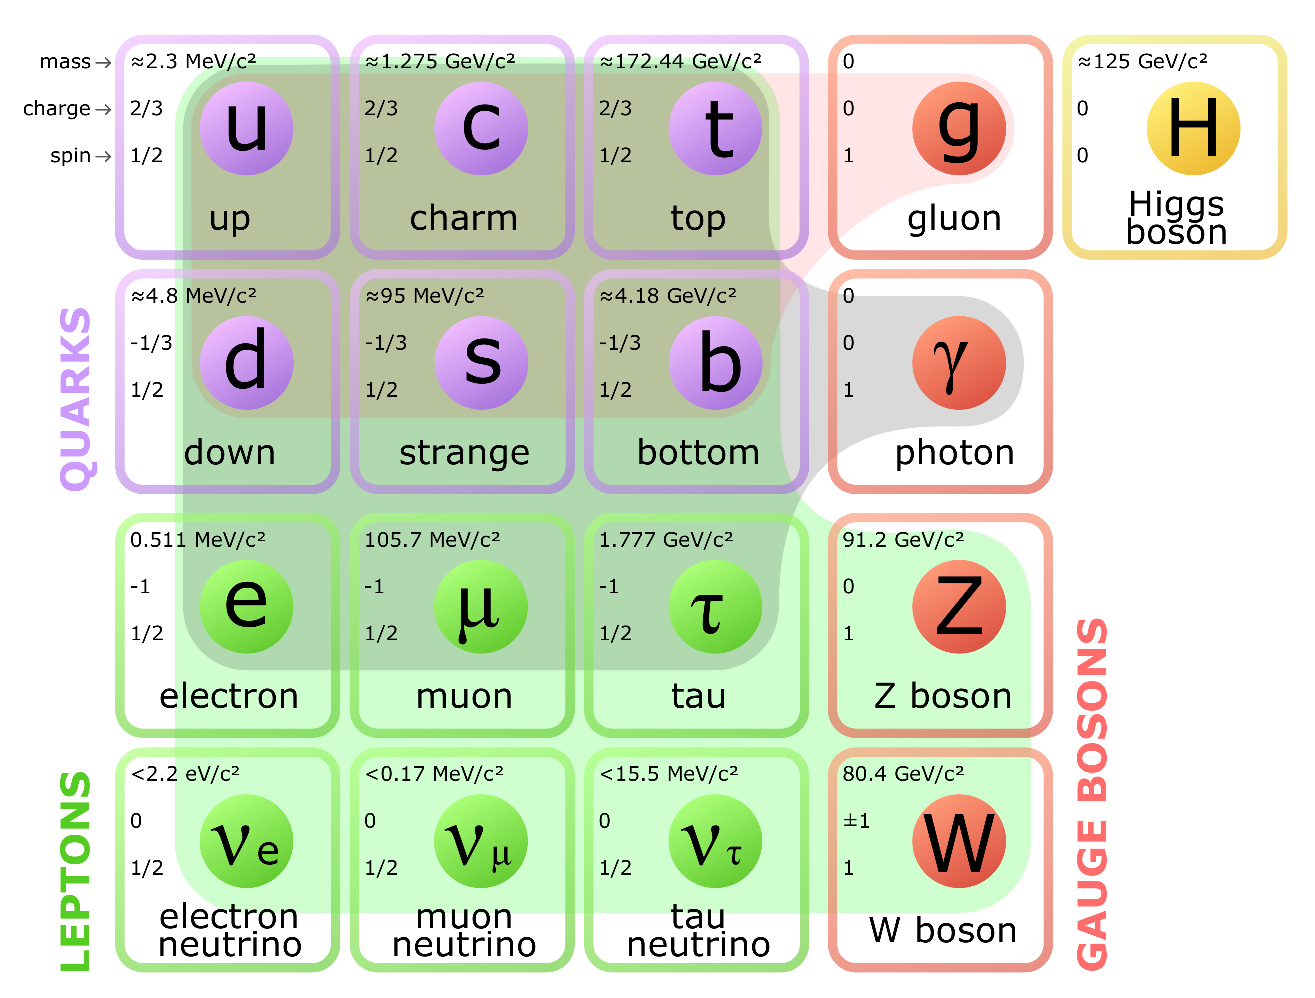
\includegraphics[width=0.6\textwidth]{figures/theory/Standard_Model_of_Elementary_Particles_modified_version.eps}
\caption[The particle content of the Standard Model]{The particle content of the Standard Model. Figure adapted from~\cite{wikipediaSM}.}
\label{fig:standard_model}
\end{centering}
\end{figure}


\subsection{The Lorentz group and particle states}

Lorentz group consists of coordinate transformations~$x^\mu = \Lambda^{\mu}_{\ \nu} x^\nu$~that preserve space-time intervals~$\mathrm{d}s^2 = \mathrm{d}x^\mu \Lambda^\mu_{\ \nu} \mathrm{d}x_\nu$, such that~$\mathrm{det}\ \Lambda = +1$~and~$\mathrm{sign}\ \Lambda^0_{\ 0} = +1$. The transformations form a group~$\mathrm{SO}^+(3,1)$, which can be decomposed~$\mathrm{SO}^+(3,1) \simeq \mathrm{SU}(2)_L \times \mathrm{SU}(2)_R$. This allows the angular momenta~$(j_1, j_2)$~of the decomposition to be used to group the fields as scalars~$(j_1=0, j_2=0)$, left and right handed spinors~$(\frac{1}{2}, 0), (0, \frac{1}{2})$ and vectors $(1, 1)$ based on their transformation properties under the Lorentz group. For example, a scalar field~$\phi(x)$~transforms as~$\phi(x) \rightarrow \phi(\Lambda^{-1} x)$, a vector field as~$A^\mu(x) \rightarrow \Lambda^\mu_{\ \nu} A^\nu(\Lambda^{-1}x)$~and a spinor field as~$\phi^\alpha(x) = S[\Lambda]^a_{\ \beta} \phi^\beta(x)$, where~$S[\Lambda]$~is a spinor built from~$4\times4$~Dirac~$\gamma$~matrices in the chiral representation.

These fields can be identified with particle states, which have a definite mass~$m$~and spin~$s$~\cite{wigner1939unitary}. According to the spin-statistics theorem, particles with integer spin (bosons) follow Bose-Einstein statistics, whereas particles with half-integer spin (fermions) follow Fermi-Dirac statistics~\cite{pauli1940connection}. 

\subsection{Relativistic quantum mechanics}
After having identified quantum fields with definite Lorentz transformation properties as the central objects in QFT, the next step is to derive dynamical relations for the free fields in order to describe the propagation of free particles.

The Klein-Gordon wave equation,

\begin{equation}
\label{eq:theory_klein_gordon}
(\partial^\mu \partial_\mu + m^2) \psi = 0
\end{equation}
which can be derived from Einstein's energy-momentum relation~$E^2 = \vec{p}^2 + m^2$~by replacing energy and momentum with operators acting on the wavefunction~$\psi$, is a manifestly Lorentz-invariant relation between energy and momentum for the quantum mechanical wavefunction. However, it admits solutions with negative energy and negative probability densities, which are unphysical.

These negative-probability states led Dirac to search for a relation linear in~$\hat{\mathbf{p}}$~and~$E$, which resulted in the Dirac equation:

\begin{equation}
\label{eq:theory_dirac}
i (\gamma^\mu \partial_\mu - m) \psi = 0
\end{equation}
where~$\gamma^\mu$~are the~$4\times4$~Dirac~$\gamma$-matrices which satisfy the Clifford algebra anti-commutation relation~$\{ \gamma^\mu, \gamma^\nu \} = \gamma^\mu \gamma^\nu + \gamma^\nu \gamma^\mu = 2 g^{\mu\nu} \mathbb{I}$~and~$\psi$~is a four-component spinor. Using~\cref{eq:theory_dirac}, we can describe the dynamics, spin and magnetic moment of free spin-half fermions. The probability densities predicted by Dirac's equation are now positive, but it still admits solutions with negative energy. In the Feynman-Stückelberg interpretation, these~$E<0$~solutions can be interpreted as negative-energy particles moving backwards in time or equivalently as anti-particles moving forwards in time. The predictions by Dirac's equation were spectacularly confirmed by the discovery of the positron in 1932~\cite{anderson1933positive}.

Both of these equations of motion can be derived from the Lagrangian using the principle of least action:

\begin{equation}
\label{eq:theory_action}
S = \int \mathrm{d}^4x\ \mathcal{L}_{\mathrm{free}},\ \delta S = 0,
\end{equation}
where~$\mathcal{L}_{\mathrm{free}}$~is the Lagrangian density for non-interacting fields for the Klein-Gordon or Dirac case respectively and the integral is taken over all possible path variations of the fields. The Dirac action for a single free spinor field can be written as

\begin{equation}
\label{eq:theory_kg_lagrangian}
\mathcal{L}_{\mathrm{Dirac}} = \bar{\psi} i \gamma^\mu \partial_\mu \psi - m \bar{\psi} \psi,\ \bar{\psi} = \psi^\dagger \gamma^0
\end{equation}
and varied with respect to~$\psi$~to derive the Dirac equation.

\subsection{Interactions via gauge theory}
The concept of interactions mediated by fields is central to QFT. In order to encode the observed particle interactions in the theory, we require the Lagrangian to have additional symmetries. In particular, if we require the laws of physics to be invariant under local transformations~$\psi(x) \rightarrow U(x) \psi(x)$, where the continuous and differentiable transformations~$U(x)$~form Lie groups, then the principle of gauge symmetry allows additional degrees of freedom corresponding to the mediator fields or gauge bosons to be naturally incorporated in the Lagrangian. First, we show how quantum electrodynamics, the relativistic quantum theory of electron-photon interaction and thus electromagnetism, arises from the gauge principle.

\subsection{Quantum Electrodynamics}
For the~$\mathrm{U}(1)$~symmetry, which corresponds to the transformation~$\psi(x) \rightarrow e^{i q\varphi(x)} \psi(x)$, in order for the Lagrangian to be invariant under this symmetry, the derivative in the momentum operator in~\cref{eq:theory_kg_lagrangian} needs to be changed to

\begin{equation}
\partial_{\mu} \rightarrow \mathcal{D}_{\mu} = \partial_{\mu} + i q A_{\mu}.
\end{equation}
This ensures that the covariant derivative $\mathcal{D}{\mu}\psi$ transforms as the field $\psi$ itself under the gauge transformation $U$.
The field~$A_{\mu}$~corresponds to a massless gauge boson with spin 1 that is coupled to the fermion field~$\psi$~via a coupling constant~$q$~in the term~$q \gamma^\mu A_\mu \psi$. The formulation of quantum electrodynamics (QED) as a gauge theory generated by the Abelian group~$\mathrm{U}(1)_{\mathrm{EM}}$~was first done by Tomonaga, Feynman and Schwinger~\cite{PhysRev.73.416, PhysRev.74.1439, PhysRev.76.769}. In QED, the spinor~$\psi$~is associated to the electron, the vector~$A_\mu$~to the photon and~$q$~is the electric charge of the fermion. 

In order to compute observable decay rates or scattering cross sections under an interaction Hamiltonian~$V$, we use Fermi's golden rule, which relates the scattering rate~$\Gamma_{fi}$~to the transition matrix element between the initial and final state derived using perturbation theory:

\begin{equation}
\label{eq:transition_matrix}
\Gamma_{fi} \propto |\mathcal{M}_{fi}|^2 \rho, \mathcal{M}_{fi} = \langle \psi_f | V | \psi_i \rangle.
\end{equation}

The matrix element in~\cref{eq:transition_matrix} is a Lorentz scalar and can be explicitly computed from the Lagrangian using Feynman rules, where we represent each term in the perturbation expansion of~\cref{eq:transition_matrix} as a graphical diagram with the ingoing and outgoing lines. The vertices and the propagators are associated with quantities that are specified by the form of the interacting Lagrangian. The basic QED interaction vertex thus allows us to construct diagrams corresponding to any QED interaction and calculate scattering cross sections for processes such as electron-electron scattering, as depicted on~\cref{fig:theory_qed}.

\begin{figure}
\begin{centering}
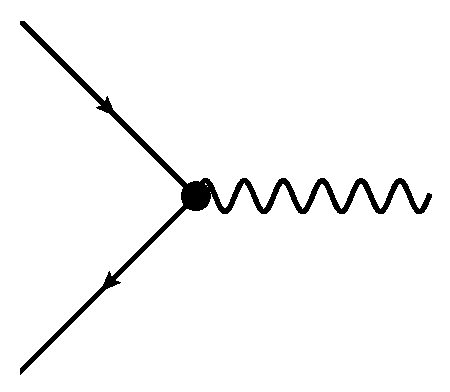
\includegraphics[width=0.3\textwidth]{figures/theory/qed_vertex.eps}
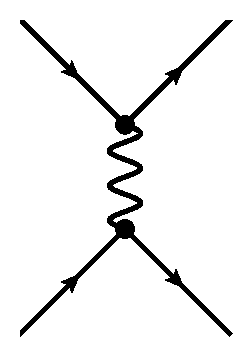
\includegraphics[width=0.2\textwidth]{figures/theory/qed_process.eps}
\caption{The QED vertex and a representative process.}
\label{fig:theory_qed}
\end{centering}
\end{figure}

It is remarkable that the gauge theory formulation of QED allows us to both recover Maxwell's equations of electromagnetism and predict the anomalous electric dipole moment of the electron, which has been confirmed to be accurate to about one part per billion~\cite{Aoyama:2007mn}. This underscores the predictive power of symmetries in the SM.

\subsection{Quantum Chromodynamics}
\label{sec:theory_qcd}
The interaction of quarks and gluons can be described by the theory of quantum chromodynamics (QCD), which arises from the invariance of the Lagrangian under a local~$\mathrm{SU}(3)_C$~symmetry, where C stands for a colour charge that is~$N_c$-valent, with~$N_c = 3$~in the SM. The spinor field transforms under this group as

\begin{equation}
\psi(x) \rightarrow \psi'(x) = \exp \bigl[ i g_s \alpha^a(x) T^a \bigr] \psi(x)
\end{equation}
where~$T^a$~are the generators of the group represented by the~$3\times3$~Gell-Mann matrices~$\lambda^a$~as~$T^a = \frac{1}{2} \lambda^a$,~$g_s$~is the gauge coupling and~$\alpha^a(x)$~are the local gauge transformations corresponding to the 8 generators. The covariant derivative can then be written as


\begin{equation}
\label{eq:theory_qcd_deriv}
\partial_\mu \rightarrow \mathcal{D}_\mu = \partial_\mu + i g_s G^a_\mu T^a
\end{equation}
where~$G^a_\mu = \partial_\mu \alpha^a(x)$~must transform as~$G^a_\mu \rightarrow G^a_\mu - \partial_\mu \alpha^a - g_s f_{ijk} \alpha^i G^j_\mu$. The last term arises due to the non-Abelian nature of QCD, which means that the generators~$T^a$~do not commute, but are instead related through the structure constants:~$[T^a, T^b] = T^a T^b - T^b T^a = 2 i f_{abc} T^c$. The Lagrangian for a single quark field can then be written as

\begin{equation}
\label{eq:theory_quark_lagrangian}
\mathcal{L}_{\mathrm{quark}} = \bar{\Psi} (i \gamma^\mu \partial_\mu - m + g_s \gamma^\mu G^a_\mu T^a) \Psi = 0
\end{equation}
and we can associate~$G^a_\mu$~to the gluons. We note that~$\Psi = (\psi_i)$~has 3 components corresponding to colour states, each of which is a 4-component Dirac spinor. The QCD quark-gluon interaction vertex is then

\begin{equation}
g_s \gamma_\mu T^a G^a_\mu~(\mathrm{q}\bar{\mathrm{q}}\mathrm{g}).
\end{equation}

At this stage,~$G^a_\mu$~is simply ga field associated with external sources, which can be made dynamical by adding a gauge-invariant term

\begin{equation}
\mathcal{L}_{\mathrm{gauge}} = - \frac{1}{2} \mathrm{Tr}\ [F^{\mu\nu} F_{\mu\nu}] 
\end{equation}
to the QCD Lagrangian, where~$F_{\mu\nu} = \partial_\mu G_\nu - \partial_\nu G_\mu + i g_s [G_\mu, G_\nu]$~with~$G_\mu = G_\mu^a T^a$~is the QCD gluon field strength tensor. The non-vanishing structure constants $f_{abc}$ imply that gluons carry colour charge and thus interact with each other, giving rise to a triple-gluon vertex (ggg) proportional to $g_s$ and a 4-gluon vertex (gggg) proportional to $g_s^2$.

The~$\mathrm{SU}(3)_{\mathrm{C}}$~symmetry of QCD thus implies the existence of a conserved trivalent colour charge, which is exchanged between quarks by 8 gluons carrying colour-anticolour in QCD vertices. As free quarks have not been experimentally detected, the colour charge is hypothesised to be confined, such that quarks are only observed bound to colourless hadrons - mesons ($\mathrm{q}\bar{\mathrm{q}}$) and baryons (qqq'). Furthermore, this means that hadrons have to be colour singlets, which for baryons, composed of 3 quarks, implies that the colour wavefunction must be totally antisymmetric under the exchange of any two quarks, since the colour  singlet~$\psi_c = \frac{1}{\sqrt{6}} (rgb - rbg + gbr - grb + brg - bgr)$~from the decomposition~$\mathbf{3}\otimes \mathbf{3} \otimes \mathbf{3} = \mathbf{10} \oplus \mathbf{8} \oplus \mathbf{8} \oplus \mathbf{1}$~is totally antisymmetric.

The success of QCD in describing the phenomenology of high-energy interactions of protons relies on a model for building hadrons out of the elementary constituents of QCD - the quarks and gluons.

\subsection{Flavour states of hadrons}
The known quarks of the SM come in 6 different flavours, grouped into 3 generations: up and down (I), charm and strange (II), top and bottom (III). The underlying reason for the SM having exactly 3 generations is unknown, but an approximate symmetry between flavours allows us to predict allowable hadronic states that can be formed from quarks. Strong interaction is approximately invariant under~$\mathrm{u} \leftrightarrow \mathrm{d}$~exchange, which implies an~$\mathrm{SU}(2)$~flavour symmetry. This group has 3 generators~$\hat{T}_i$~that can be represented as~$2\times2$~Pauli spin matrices. This means that for a given flavour state~$\psi$, the quantized isospin~$I_3 \leftrightarrow \hat{T}_3$~and the total isospin~$I \leftrightarrow \hat{T}^2$~are conserved in analogy to spin, and can therefore be used to label composite flavour states of quarks as~$\phi(I, I_3)$.

We can construct the flavour wavefunction proton, which contains 3 valence quarks (uud), by combining 3 isospin doublets~$\mathbf{2} \otimes \mathbf{2} \otimes \mathbf{2} = \mathbf{4} \oplus \mathbf{2}$, which results in a spin~$I=3/2$~quadruplet and two spin~$I=1/2$~doublets~$\phi_A=\frac{1}{\sqrt{2}}(\mathrm{udu} - \mathrm{duu})$~and~$\phi_S = \frac{1}{\sqrt{6}}(2 \mathrm{uud} - \mathrm{duu} - \mathrm{udu})$, that are (anti)symmetric under the exchange of the first two quarks. The proton wavefunction is then a superposition of the two flavour doublets, multiplied by the corresponding (anti)symmetric wavefunctions for the spin states, such that the flavour-spin wavefunction is completely symmetric under the exchange of any two quarks. This, combined with the completely antisymmetric colour wavefunction as described in~\cref{sec:theory_qcd}, guarantees that the proton wavefunction is completely antisymmetric under the exchange of any two quarks.

The~$\mathrm{SU}(2)$~isospin symmetry of flavour allows us to write down the wavefunction of the proton in the ground state and predict the existence and approximate masses of the excited states such as the~$\Delta$-baryons. It is not an exact symmetry, as illustrated by the difference in the proton and neutron masses, which should vanish under precise~$\mathrm{SU}(2)$~isospin symmetry, but nevertheless underscores the role of symmetries in describing hadronic states. Further hadronic states can be described by the $\mathrm{SU}(3)$ model, where the u, d and c quarks are grouped into a triplet

\subsection{Weak interaction}
The weak force is responsible for radioactive~$\beta$-decay and is the only fundamental interaction known to violate parity~\cite{Wu:1957my}. The weak interaction couples neutrinos to charged leptons and up-type quarks to down-type quarks via the exchange of massive vector bosons, the charged W and the neutral Z. At low energy ($q \ll m_W$) and before the observation of parity violations, the weak force was modelled as a Fermi theory with a matrix element $\mathcal{M} = G_F g_{\mu\nu} [\bar{psi}_3 \gamma^\mu \psi_1][\bar{psi}_4 \gamma^\mu \psi_2]$ corresponding to a point interaction of 4 fermions proportional to the Fermi constant $G_F$. After the observation of parity violation, the weak interaction vertex needed to be modified to include axial vector coupling in addition to vector coupling, such that it is proportional to $g \gamma^\mu(1 - \gamma^5)$, such that the vertex has a vector minus axial vector (V-A) structure. The $\gamma^5$ operator serves to project out the left (right) handed (anti)-particle chiral states, such that only these states interact via weak boson exchange.

The weak interaction can be described in the SM as a~$\mathrm{SU}(2)_L$~gauge symmetry. The left-handed fermions form doublets~$(\nu_L, \mathrm{\ell}_L)$~for leptons and~$(q_L, q'_L)$~for quarks, whereas right-handed fermions $\ell_R$, $\nu_R$, $q_R$ are singlets under weak isospin. The generators~$T_i$~of~$\mathrm{SU}(2)_L$~are related to the 3 Pauli matrices~$T_i = \frac{1}{2}\sigma_i$, which can then be associated to 2 charged vector boson fields that mediate the weak force:~$W^{\pm}_\mu=\frac{1}{\sqrt{2}}(W^1_\mu \mp i W^2_\mu)$. The gauge structure predicts the existence of a massive electrically neutral vector boson $W^3_\mu$, which can be associated to the SM Z boson through electroweak unification.

\subsection{Electroweak unification}

The weak and electromagnetic forces both suggest an electrically neutral boson, so the physically observed states of the photon and the Z-boson must be a superposition of the two, implying a connection between the weak and electromagnetic forces. The mixing between the neutral gauge boson states can be expressed as $A = B \cos{\theta_W} + W^3 \sin{\theta_W}$ and is characterized by the weak mixing angle $\theta_W = \tan^{-1}{g'/g}$ between a new $\mathrm{U}(1)_Y$ gauge field B with a coupling $g'$ and the neutral component of the weak force $W^3$. In the Glashow-Weinberg-Salam theory of electroweak unification, the Lagrangian is symmetric under the group~$\mathrm{SU}(2)_L \times \mathrm{U}(1)_Y$, whereas the vacuum state is symmetric only under the QED gauge symmetry~$\mathrm{U}(1)_{\mathrm{EM}}$. In the unified theory, it is necessary to introduce a new quantum number~$Y$, the hypercharge, which is equal for both components of the~$\mathrm{SU}(2)_L$~doublets, so that the left-handed doublets would be invariant under both~$\mathrm{SU}(2)_L$~and~$\mathrm{U}(1)_Y$~symmetries. The observed electric charges of the fermions are then related to the weak hypercharge~$Y$~and weak isospin~$I_3$~by~$Q = I_3 + Y/2$.

The theory of electroweak unification was confirmed by the discovery of the Z-boson by the UA1 experiment at the SPS collider~\cite{Arnison:1983mk}, which couples to both left-handed and right-handed fermions. This has allowed the weak mixing angle~$\theta_W$~between the neutral vector boson states to be measured. Furthermore, the decay~$\mathrm{Z} \rightarrow \nu \bar{\nu}$~can be used to determine the number of light neutrino generations by measuring the total width of the Z-boson~$\Gamma_Z$~and the decay widths to visible fermions - the charged leptons~$\mathrm{e}^\pm, \mathrm{\mu}^\pm, \mathrm{\tau}^\pm$~and quarks. The principle of local gauge invariance has great predictive power for the overall structure of the observed interactions, but it does not account for the mechanism by which electroweak symmetry breaking (EWSB) is realized nor the mass of the~$\mathrm{W}^\pm$~and Z bosons, which would violate gauge invariance. In order to incorporate these phenomena, we turn to the Higgs mechanism.

\subsection{Higgs mechanism}
We can introduce mass terms for the heavy gauge bosons by coupling them to two complex scalar fields arranged in a weak isospin doublet~$\phi = \frac{1}{\sqrt{2}} (\phi^+\ \phi_0)^T$. The Lagrangian density for this scalar field is~$\mathcal{L}_{\phi} = (\partial_\mu \phi)^\dagger (\partial^\mu \phi) - V(\phi)$, where the Higgs potential~$V(\phi) = \mu^2 (\phi^\dagger \phi) + \lambda (\phi^\dagger \phi)^2$~has degenerate minima~$\phi^\dagger \phi = v^2 / 2 = -\mu^2/2\lambda$~for~$\mu^2 < 0$. If the physical vacuum state does not have the same symmetries as the Lagrangian, then it is possible to introduce gauge-invariant mass terms for gauge bosons and fermions.

The Higgs field couples to the gauge fields through the kinetic term~$(\partial_{\mu} \phi)^\dagger (\partial^\mu \phi)$, which is made gauge invariant by~$\partial_\mu \rightarrow D_\mu = \partial_mu + i g T^a W_\mu^a + i g' Y B_\mu / 2$. The vacuum state is then chosen to be~$\langle 0|\phi|0\rangle = \frac{1}{\sqrt{2}} (0\ v)^T$, so the Higgs field can be expanded around the vacuum, resulting in a massive scalar field~$\eta$~and 3 massless Goldstone fields~$\phi_1, \phi_2, \phi_3$. The Goldstone bosons are removed from the Lagrangian by fixing the gauge, such that they correspond to the degrees of freedom of longitudinal polarization states of the Z and~$\mathrm{W}^\pm$~bosons. The masses of the gauge bosons can then be written as~$M_W = \frac{1}{2} g v$~and~$m_Z = \frac{1}{2} g v / \cos{\theta_W}$. The theory of EWSB predicts~$m_W / m_Z = \cos{\theta_W}$, which has been confirmed experimentally~\cite{ALEPH:2005ab}.

The explicit mass terms for fermions in the form of~$m \bar{\psi} \psi$~are not gauge invariant. By arranging the left-handed fermions in a~$\mathrm{SU}(2)$~doublets~$L$~and the right-handed fermions in singlets~$R$, the mass terms for Dirac fermions can be introduced through spontaneous symmetry breaking through the terms~$y_f \bar{L}\phi R + y_f (\bar{L}\phi R)^\dagger$~for down-type leptons $e^\pm$, $\mu^\pm$, $\tau^\pm$ and quarks $\mathrm{d}$, $\mathrm{s}$~and $\mathrm{b}$. The constant $y_f = \sqrt{2} m_f / v$ is the Yukawa coupling of the fermions, which has to be fixed from the experimental determination of the masses. A conjugate Higgs doublet~$\phi_c = -i\sigma_2 \phi^*$~is used to give the mass terms for the up-type quarks. From this mechanism, the Yukawa coupling of the top quark is found to be compatible with unity, a scale very different from the rest of the quarks.

To summarize, the Higgs mechanism can accommodate the observed masses of heavy gauge bosons and fermions in a unified electroweak theory. It predicts the existence of a massive scalar boson, which can decay to fermions through~$\mathrm{H} \rightarrow \mathrm{f} \bar{\mathrm{f}}$~or bosons through~$\mathrm{H} \rightarrow \mathrm{W}^+ \mathrm{W}^-$ and ~$\mathrm{H} \rightarrow \mathrm{Z} \mathrm{Z}$, and through higher-order processes to $\mathrm{H} \rightarrow \gamma \gamma$.

\subsection{Top quark physics}
The top quark is the most massive particle in the SM, with $m_t = 173.34 \pm 0.27~\mathrm{(stat)} \pm 0.71~\mathrm{(syst)}$~\cite{ATLAS:2014wva}, such that it is kinematically allowed to decay through weak interaction $\mathrm{t} \rightarrow \mathrm{b} \mathrm{W}^+$. This is the primary decay mode, since $|V_{tb}| \gg |V_{ts}|, |V_{td}|$ from the CKM mass matrix and the hadronization timescale $\Lambda_{QCD}^{-1} \simeq 10^{-23}~\mathrm{s}$ is much larger than the top quark lifetime $\tau \simeq 10^{-25}~\mathrm{s}$. This means that the top quark mass can be measured accurately from a relatively small amount of decay products, among which is the b~quark with a distinctive experimental signature, as opposed to light quarks, which hadronize into potentially hundreds of mesons.

The top quark was discovered in 1995 at the CDF experiment at Tevatron~\cite{Abe:1995hr} and is now ubiquitous at the LHC, where it is produced primarily through gluon-gluon fusion in the form of top quark pairs.

%%%%%%%%%%%%%%%%%%%%%%%%%%%%%%%%%%
%%%%%%%%%%%%%%%%%%%%%%%%%%%%%%%%%%
%%%%%%%%%%%%%%%%%%%%%%%%%%%%%%%%%%

\section{The Standard Model at colliders}
\subsection{The parton model}
Through the study of deep inelastic scattering (DIS) experiments, where an electron transfers sufficient energy~$Q^2$~to a proton for it to break up in the process~$\mathrm{e}^- \mathrm{p} \rightarrow \mathrm{e}^- \mathrm{X}$, with $\mathrm{X}$ being a proton remnant, it was possible to establish that the electrons scatter elastically off point-like spin-half constituents of the proton, the partons. This can be seen as an analogy to the Rutherford experiment, where electrons were scattered off the nucleus of an atom to reveal the point-like structure of the nucleus within. By identifying the partons as the quarks from QCD, electron-proton interactions can thus be described in terms of the more fundamental electron-quark interactions.

Furthermore, by measuring the~$Q^2$-dependence of the QCD coupling constant~$\alpha_s(Q^2) = g_s^2 / 4\pi$~ experimentally and from theoretical considerations of QCD~\cite{PhysRevLett.30.1343,PhysRevLett.30.1346}, it has been possible to establish that at high~$Q^2$, the coupling constant~$\alpha_S(Q^2)$~becomes small ($\alpha_s \simeq 0.1$), such that quarks can be treated as free particles in the asymptotic limit. The~$Q^2$-dependence of~$\alpha_s$~can be seen on~\cref{fig:theory_alphas_running}, confirming the QCD prediction of asymptotic freedom. Only when the coupling~$\alpha_S(Q^2)$~is sufficiently small can perturbative QCD (pQCD) be used to compute cross-sections of the underlying processes. However, it is important to note that the magnitude of the strong coupling constant in the perturbative, high $Q^2$ regime is still significantly larger than the electromagnetic coupling constant, which means that higher-order loop processes are important in QCD.

The other feature of the running of $\alpha_s$ is that at a momentum scale comparable to typical hadron sizes~$\Lambda_{\mathrm{QCD}} = 0.1,\dots0.3$~GeV, the coupling constant becomes singular, implying the breakdown of perturbative QCD at~$Q < \Lambda_{\mathrm{QCD}}$. This means that in processes with low energy scales such as the production or interaction of hadrons, non-perturbative dynamics of QCD become important.

\begin{figure}
\begin{centering}
\includegraphics[width=0.5\textwidth]{figures/theory/asq-2015.pdf}
\caption[The measured values of~$\alpha_S(Q^2)$ compared to NLO QCD]{The measured values of the strong coupling~$\alpha_S(Q^2)$, compared to the prediction from NLO QCD. We see that $\alpha_S$ decreases as the momentum scale $Q^2$ increases, reflecting the asymptotically free nature of QCD. Figure from~\cite{Patrignani:2016xqp}.}
\label{fig:theory_alphas_running}
\end{centering}
\end{figure}

In order to model a proton-proton interaction with a hard scattering, such as the Drell-Yan process~$\mathrm{q} \bar{\mathrm{q}} \rightarrow \ell^+ \ell^-$~at high~$Q^2$, we describe the protons in terms of parton distribution functions~(PDFs)~$f_a^{\mathrm{p}}(x)$, which follows from the factorization theorem in QCD~\cite{collins1989perturbative}. These specify the fraction of proton momentum~$x$~carried by a quasi-free constituent quark or gluon~$a$~and factorise the proton-proton interaction to a hard interaction between quarks and gluons, as depicted on~\cref{fig:theory_pdf_factorization}. This allows us to write the factorised cross-section for the process $\mathrm{p} \mathrm{p} \rightarrow cd$ as

\begin{equation}
\label{eq:theory_pdf_factorization}
\mathrm{d}\sigma(\mathrm{p}\mathrm{p} \rightarrow cd) = \int_0^1 \mathrm{d}x_1 \mathrm{d}x_2 \sum_{a,b} f_a^{\mathrm{p}}(x_1, \mu_F^2) f_b^{\mathrm{p}}(x_2, \mu_F^2)\ \mathrm{d}\hat{\sigma}^{ab \rightarrow cd} (Q^2, \mu_f^2),
\end{equation}
which is evaluated at the factorisation scale~$\mu_F^2$. In a qualitative sense, emissions with a transverse momentum above $\mu_F$ are accounted in the cross-section, otherwise, they are contained in the PDF. As it is not possible to describe the structure of hadrons and the PDFs perturbatively, they have to be determined from experimental data in terms of $x$ and $\mu_F^2$. The proton is a dynamical system of bound quarks that interact strongly via virtual gluon exchange, so the protons are found to contain a \textit{sea} of gluons and quarks and anti-quarks from the vacuum fluctuations of~$\mathrm{g} \rightarrow \mathrm{q} \bar{\mathrm{q}}$~in addition to the up and down \textit{valence} quarks expected from flavour symmetry. The PDFs at different scales $\mu_F$ are related through the DGLAP\footnote{Dokshitzer, Gribov, Lipatov, Altarelli and Parisi} evolution equations, which result from QCD corrections and involve splitting kernels that arise from the basic QCD vertices. This allows us to deduce the PDFs at a certain scale from measurements at a different scale, making it possible to use data from various collider experiments in combined PDF fits and for making predictions at the LHC. The PDFs for protons at different factorization scales are shown on~\cref{fig:proton_pdf}.

\begin{figure}
\begin{centering}
\includegraphics[width=0.8\textwidth]{figures/theory/pdf.pdf}
\caption[The parton distribution functions for protons.]{The parton distribution functions for protons at $\mu_F^2 = 10~\mathrm{GeV}^2$ (left) and $\mu_F^2 = 10^4~\mathrm{GeV}^2$. We see that at higher momenta $\mu_F$ and low $x$, the proton consists almost entirely out of gluons. Figure from~\cite{Patrignani:2016xqp}.}
\label{fig:proton_pdf}
\end{centering}
\end{figure}

\subsection{Jet physics}
In a process where QCD partons (quarks or gluons) are created, we cannot observe them directly, since colour confinement forbids the existence of isolated coloured states. Events with quarks and gluons in the final state can be observed experimentally as collimated jets of hadrons. This feature, which emerges from the short to long distance evolution of QCD, makes it possible to make measurements on macroscopic distance scales and connect them to otherwise inaccessible microscopic quantities such as the parton momenta or quantum numbers~\cite{Sterman:1977wj}.

Jets are formed through the creation of a parton with high virtuality $Q^2$, which undergoes showering in until it reaches a soft hadronization scale, where non-perturbative processes create stable hadrons, primarily charged and neutral pions ($\pi^\pm$, $\pi^0$) and neutral baryons. Due to the soft and collinear divergences in the QCD splitting functions, the jets are collimated along the direction of the original parton momentum.

In order to compare QCD predictions to experimental data, jet-related observables must be defined in such a way that they are infrared and collinear safe, but also practical to compute for events with very high jet multiplicities that are expected in hadron colliders. This can be done using sequential recombination, where energy clusters with momenta $k_{t,i}$ and corresponding distances $d_{ij} = \mathrm{min}(k_{t,i}^{2p}, k_{t,}^{2p}) \Delta_{ij} / R^2$ are recombined until stable jets can be formed. These jet algorithms are characterized by the jet radius parameter $R$ and the parameter $p$, where $p=-1$ corresponds to the \textit{anti-$k_T$} algorithm~\cite{Cacciari:2008gp}.

\subsection{Monte Carlo event generators}
In order to compute experimental observables such as differential distributions from the underlying theory of the SM, we typically use Monte Carlo (MC) simulators. Although inclusive observables and in some cases differential distributions can be calculated analytically, it is in general not possible to apply experimental cuts, therefore the observable phase space is sampled probabilistically to generate simulated events, which can be compared to the measurement~\cite{Sjostrand:2006za}.

The MC simulators generally work in several stages, starting with importance sampling the phase space of the hard scattering process, such that events occur with probability proportional to $|\mathcal{M}|^2$. This is simple at leading order, but in higher orders, the cancellations between real and virtual contributions need to be accounted and the procedure becomes more complicated~\cite{Frixione:2002ik}. The hard process defines the overall energy flow in the event.

The hard process is followed by the simulation of the parton shower, which evolves down from the hard scale by gluon emission or $\mathrm{g} \rightarrow \mathrm{q} \bar{\mathrm{q}}$ splittings. Showering is generally process-independent, but may depend on the inherent momentum scales in the process. At a scale of around 1 GeV, hadronization takes over, which is usually treated using phenomenological models for the non-perturbative dynamics. The overall multiplicity of final state particles is defined by the hadronization models.

Additional radiation from gluon emission and splitting can be generated either at the level of the hard matrix element or in the parton shower in initial (ISR) or final state radiation (FSR). The matching between these two stages is therefore crucially important in accurately predicting the differential distributions, especially for events with high jet multiplicities. Furthermore, all MC implementations contain a number of free parameters, which need to be tuned to experimental data.

%%%%%%%%%%%%%%%%%%%%%%%%%%%%%%%%%%
%%%%%%%%%%%%%%%%%%%%%%%%%%%%%%%%%%
%%%%%%%%%%%%%%%%%%%%%%%%%%%%%%%%%%

\section{Higgs phenomenology}
\subsection{Higgs at the LHC}
The discovery of the Higgs boson with $m_H \simeq 125$~GeV in 2012 at the LHC by the CMS~\cite{Chatrchyan:2012xdj} and ATLAS~\cite{Aad:2012tfa} collaborations confirmed the basic mechanism of EWSB and mass generation and completed the particle spectrum of the SM. Following this, a new experimental and theoretical program has opened in experimentally verifying the properties of the Higgs boson. In particular, it should be established whether Higgs boson couples to SM gauge bosons and fermions as expected by observing these processes directly. In Run I of the LHC, the coupling of the Higgs boson to gauge bosons have been established fairly precisely, however, to be able to determine the couplings to fermions, Run II data of the LHC will be necessary~\cite{Khachatryan:2016vau}.

Beyond establishing the existence of the predicted production and decay channels, a crucial test of the Higgs mechanism is determining the coupling strengths of the new scalar field to SM fields and comparing them to the SM predictions. The top quark Yukawa coupling~$y_t$~, which is much larger than that of lighter quarks, determines the evolution of the Higgs self coupling~$\lambda$~under renormalization and is currently only known indirectly, as will be discussed further in~\cref{sec:top_higgs}.

\subsection{Production modes}
The main production modes of the Higgs boson at the LHC, show on~\cref{fig:higgs_xs}, are through gluon-gluon fusion (ggF), with a cross-section of~$\sigma_{\mathrm{ggF}} = 48.6^{+2.2}_{-3.6}\pm1.6~(\mathrm{PDF})$~pb, weak or vector boson fusion (VBF) with a cross-section $\sigma_{\mathrm{VBF}} = 3.78^{+2\%}_{-2\%}$~pb, associated production with vector bosons (VH) with~$\sigma_{\mathrm{WH}} = 1.37^{+2\%}_{-2\%}$~pb,~$\sigma_{\mathrm{ZH}} = 0.88^{+5\%}_{-5\%}$~pb and through the associated production with top quark pairs (\ttH) with $\sigma_{\ttH} = 0.51^{+9\%}_{-13\%}$~pb or with a single top quark~(tH). We note that the difference between the ggF and~\ttH~production modes is roughly 2 orders of magnitude.

\begin{figure}
\begin{centering}
\includegraphics[width=0.6\textwidth]{figures/theory/PDG.eps}
\caption[Tree-level Feynman diagrams for Higgs production]{The generic tree-level Feynman diagrams for Higgs boson production: the gluon fusion process (ggF) on (a), vector boson fusion on (b), associated production with vector bosons (VH) on (c) and associated production with top quarks (\ttH) on(d). Figure from the PDG~\cite{Patrignani:2016xqp}.}
\label{fig:higgs_production}
\end{centering}
\end{figure}

\begin{figure}
\begin{centering}
\includegraphics[width=0.4\textwidth]{figures/theory/Higgs_XS_7-14TeV-2016.eps}
\caption[The production cross-section of the Higgs boson]{The production cross section of the SM Higgs boson with $m_H = 125$~GeV as a function of~$\sqrt{s}$ along with theoretical uncertainties. Figure from the PDG~\cite{Patrignani:2016xqp}.}
\label{fig:higgs_xs}
\end{centering}
\end{figure}

The ggF production proceeds predominantly via the top quark loop and is known to N3LO. This was the main production mode for the initial observation and discovery with the~$\mathrm{H} \rightarrow \gamma \gamma$,~$\mathrm{H} \rightarrow \mathrm{W}^+\mathrm{W}^- \rightarrow \mathrm{e} \mathrm{\nu} \mathrm{\mu} \mathrm{\nu}$~and~$\mathrm{H} \rightarrow \mathrm{Z}\mathrm{Z} \rightarrow 4\ell$ signatures, which are important for the measurement of the production cross-section,~$J^P$~and mass of the Higgs boson. It also serves as an indirect constraint on the top-Higgs Yukawa coupling, due to the presence of the top quark loop in ggF. For the direct decay of the Higgs boson to fermions, additional production modes have to be considered. The VBF mode, where two (anti)quarks scatter by exchanging a weak boson in~$\mathrm{qq} \rightarrow \mathrm{qqH}$~is important both for discovery and determination of the couplings, as it can be distinguished from QCD background through the presence of two jets in the opposite forward regions of the detector originating from the scattered quarks. The VH mode allows the use of leptonic decays of the W/Z bosons to reduce the multijet background, such that this mode has recently been used to establish the~\Hbb~decay~\cite{Aaboud:2017xsd}. While inclusive ggF measurements are already sensitive to the top quark Yukawa coupling~$y_t$, the~\ttH~and tH channels can be used to probe~$y_t$~directly, such that they provide an important independent verification of the mass generation mechanism for the top quark.

\subsection{Decay channels}
The Higgs boson decays to SM particles with decay widths~$\Gamma$~that are proportional to the mass of the daughter particles. For~$m_H
\simeq 125$~GeV, the dominant decay channels are the decay to bottom quarks~\Hbb~with a branching ratio~$\mathrm{BR} = \Gamma/\Gamma_{H} = 0.584 \pm 3.3\%$, the decay to an on-shell and an off-shell W-boson~$\mathrm{H}\rightarrow \mathrm{W} \mathrm{W}^*$~($\mathrm{BR} = 0.214\pm4.3\%$) and the decay to tau leptons~$\mathrm{H} \rightarrow \mathrm{\tau}^+ \mathrm{\tau}^-$~($\mathrm{BR} = 0.063 \pm 5.7\%$). Through loop-induced processes, which are enhanced by the large top quark mass, the Higgs boson can also decay to massless particles in the channels~$\mathrm{H} \rightarrow \mathrm{g} \mathrm{g}, \mathrm{\gamma}\mathrm{\gamma}$ with non-negligible branching fractions. The branching ratios for a SM Higgs boson as a function of~$m_H$~can be seen on~\cref{fig:higgs_br}.

\begin{figure}
\begin{centering}
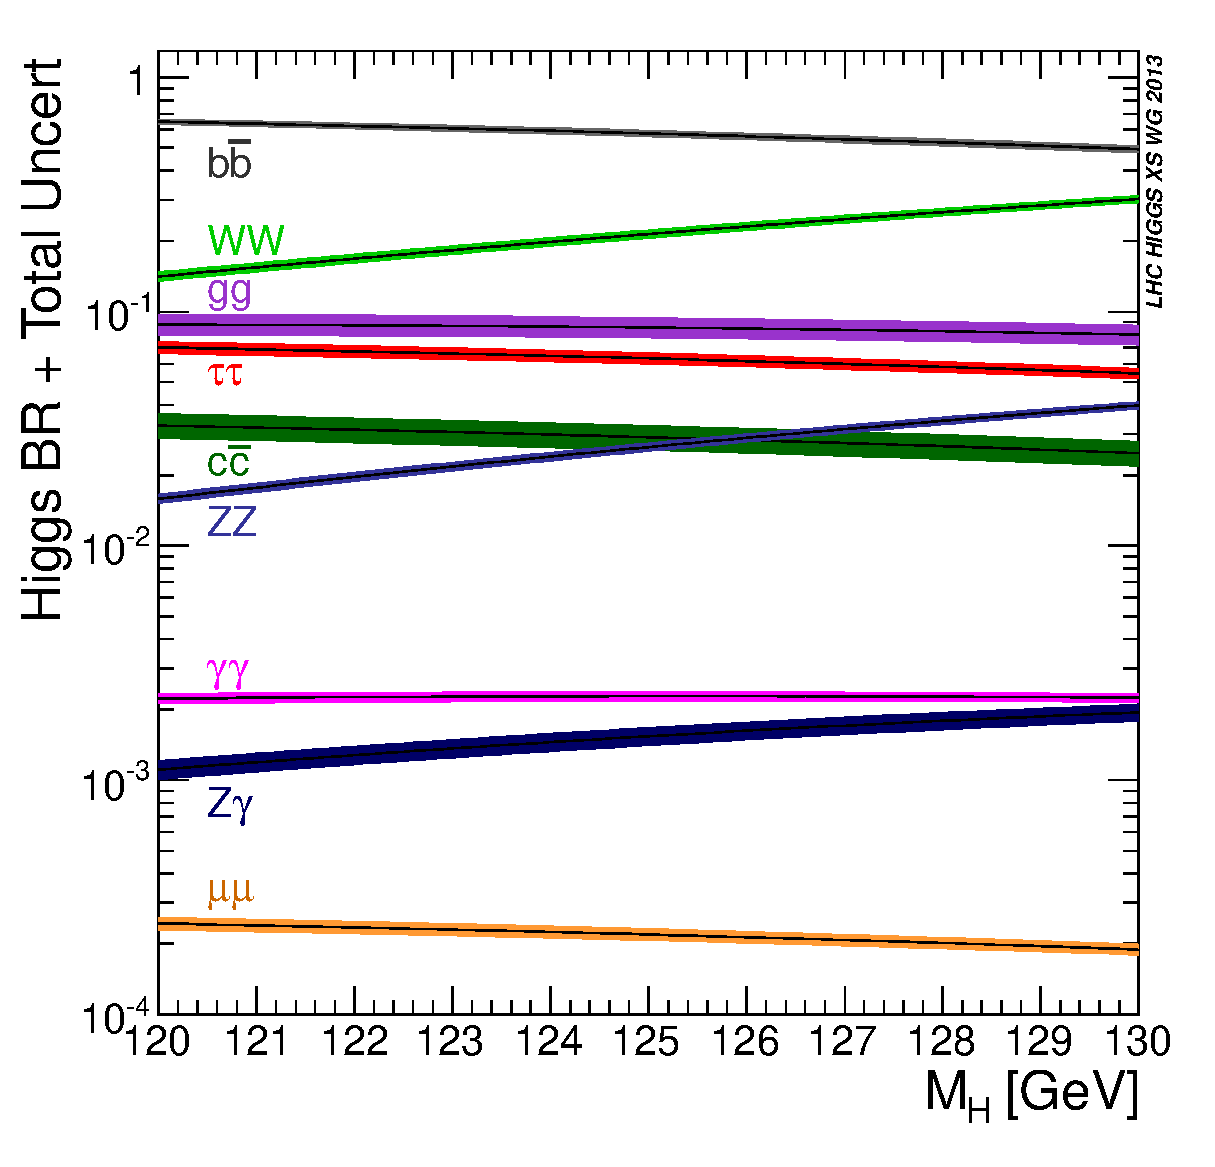
\includegraphics[width=0.4\textwidth]{figures/theory/higgs_br.eps}
\caption[The branching ratios of the Higgs boson]{The branching ratios of the SM Higgs boson around~$m_H = 125$~GeV along with the theoretical uncertainties. Figure from the PDG~\cite{Patrignani:2016xqp}.}
\label{fig:higgs_br}
\end{centering}
\end{figure}

\subsection{Experimental characterization}
Accurate predictions for the Higgs boson production cross sections and branching ratios for decays allow experimental data to be interpreted and the properties of the Higgs boson to be measured in various channels. The mass~$m_H$~has been measured most accurately in the~$\mathrm{H}\rightarrow\mathrm{\gamma}\mathrm{\gamma}$~and~$\mathrm{H} \rightarrow \mathrm{Z}\mathrm{Z} \rightarrow 4\ell$~channels, with a combined value of~$m_H = 125.09 \pm 0.21~(\mathrm{stat}.) \pm 0.11~(\mathrm{syst})$~GeV, dominated by statistical uncertainties, with the photon momentum scale uncertainties being the most significant systematic uncertainty~\cite{Aad:2015zhl}. The spin and parity~$J^P$~of the Higgs boson are probed independently of the mass and total cross section and are found to be compatible with the SM~$0^+$ hypothesis, excluding the pseudoscalar hypothesis at a~$98-99\%$ confidence level~\cite{Khachatryan:2014kca,Aad:2013xqa}. The width of the Higgs boson cannot be measured directly at the LHC, since the mass resolution in the diphoton and~$4\ell$~channels is $1-2$~GeV, 3 orders of magnitude larger than the expected SM line width $\Gamma_H = 4.2$~MeV. However, it can be constrained by comparing the on-shell and off-shell~$\mathrm{H} \rightarrow \mathrm{VV}$~cross sections, thus setting upper limits on~$\Gamma_H$~that are around 5-6 times the SM value~\cite{Khachatryan:2014iha}.

It is important to experimentally confirm that the coupling strengths of the Higgs boson to SM particles correspond to those predicted by the SM. Any deviation from the values predicted by the SM Higgs mechanism could thus signal physics beyond the SM (BSM). The simplest way to experimentally characterize discrepancies in the couplings is the so-called~$\kappa$-framework~\cite{Heinemeyer:2013tqa}, where the couplings to SM particles are rescaled by factors~$\kappa_i$~for~$i \in \{\mathrm{Z}, \mathrm{W}, \mathrm{f}, \mathrm{g}, \mathrm{\gamma}, \mathrm{Z\gamma}\}$~which can be determined from signal strength~($\mu = \sigma / \sigma_{\mathrm{SM}}$)~measurements, without modifying the SM structure of the theory. In this formalism, the~\ttH~ signal strength modified is given by~$\mu_{\ttH} = \kappa_{\mathrm{t}}^2$. The CMS and ATLAS collaborations have extracted these signal modifier values from Run I data in a combined fit, with the results shown on~\cref{fig:higgs_kappa}. The couplings, while compatible with the SM, have significant uncertainties, in particular for~$\kappa_t$, thus paving the way for Run II measurements with improved sensitivity.

\begin{figure}
\begin{centering}
\includegraphics[width=0.8\textwidth]{figures/theory/CMS-HIG-15-002_Figure_015.pdf}
\caption[The Higgs signal strength modifier factors as measured by CMS and ATLAS]{The combined signal strength modified factors~$\kappa$~from the CMS and ATLAS collaborations with Run I data. Figure from~\cite{Khachatryan:2016vau}.}
\label{fig:higgs_kappa}
\end{centering}
\end{figure}

While the~$\kappa$-framework is relatively simple to apply for small deviations in signal strength, the clear short-coming of this approach is that any BSM physics would necessarily change the structure of the theory, rendering the results potentially invalid. In particular, the above approach assumes that the loop contributions in ggF and $\mathrm{H} \rightarrow \mathrm{\gamma} \mathrm{\gamma}$ are not modified by new physics. Furthermore, differences in kinematic distributions, such as the Higgs transverse momentum distribution, cannot be captured in the~$\kappa$~framework. Therefore, it has been suggested to use either Higgs pseudo-observables~\cite{Gonzalez-Alonso:2014eva} or effective field theories (EFT) to further parametrize any possible deviations from the SM~\cite{Buchmuller:1985jz,Grzadkowski:2010es}.

\subsection{Top-Higgs coupling}
\label{sec:top_higgs}
In the SM, the coupling between the top quark and Higgs boson is predicted to be~$y_t = \sqrt{2} m_t / v$, which can be verified by measuring the cross sections of top quark pair associated Higgs production. This makes that the direct determination of the top-Higgs coupling in~\ttH~a test of the EWSB model at natural scale where~$y \simeq 1$. 

\subsubsection{Vacuum stability}
The top-Higgs coupling plays an important role in vacuum stability, since it controls the evolution of the self-coupling~$\lambda$~of the Higgs potential through renormalization evolution $\frac{\mathrm{d}\lambda}{\mathrm{d}\ln{\mu}}$, where it gives a quartic negative contribution. In particular, if~$y_t$~is sufficiently large but well within the bounds set by experimental uncertainties, the self-coupling~$\lambda$~becomes negative at a renormalization scale~$\mu$~below the Planck scale~$M_{\mathrm{Pl}} = \sqrt{\bar{h}c / G} \simeq 10^{19}~\mathrm{GeV}$, where gravitation becomes important in QFT. This means that the Higgs potential develops an additional minimum, which would possibly make the SM vacuum state metastable, depending on the exact values of~$m_H$~and~$m_t$~\cite{Degrassi:2012ry}. Given that the we have not observed a transition between vacuum states, this would imply the existence of new physics to prevent this. Since the scale where the scalar self coupling becomes negative depends strongly on~$y_t$, an accurate determination of~$y_t$~can help to pinpoint the scale of new physics in the absence of clear BSM signals~\cite{Bezrukov:2014ina} and establish whether the vacuum is stable on cosmological timescales.

\subsubsection{Anomalous couplings}
Furthermore, the top-Higgs coupling, which is purely scalar in the SM, can be extended quite generally to contain scalar and pseudoscalar interactions, making it possible to use results from~\ttH~for setting direct constraints on anomalous top-Higgs couplings~\cite{Kobakhidze:2016mfx}. Such anomalous couplings can arise from the two-Higgs doublet model that appears in several BSM scenarios, such as supersymmetry or axions~\cite{Branco:2011iw} or from models with a composite Higgs~\cite{Liu:2017dsz}.

\subsection{Present results on~\ttH}
Both the CMS and ATLAS collaborations have searched for~\ttH~in Run I and Run II of the LHC by measuring $\mu = \sigma_{\ttH} / \sigma_{\mathrm{SM}}$ in a~\ttH-enriched region using different Higgs decay channels, with the~$\mathrm{H} \rightarrow \mathrm{WW^*},\mathrm{ZZ^*} \rightarrow \mathrm{multilepton}$,\Hbb and~\Htautau~decay channels giving the highest sensitivity in Run II, followed by~\ttH-tagged~\Hgg~decay. The results are summarized in~\cref{tab:tth_results}. The analyses are systematically dominated and quite involved in terms of statistical methods, but a recent combination by ATLAS while this work was in preparation has been able to reach a measured cross-section of $\sigma_{\ttH} = 590^{+160}_{-150}~\mathrm{fb}$, compared to the SM value of~$\sigma_{\ttH}^{\mathrm{SM}} = 507^{+35}_{-50}$, with the equivalent measurement on the CMS side in the \Hbb~channel being a major part of the thesis.


\begin{table}[h!]
\begin{center}
\begin{tabular}{c|cc}
\hline
decay channel & CMS & ATLAS \\
\hline
\multirow{3}{*}{\Hbb} & $\mu = -0.19 \pm 0.45~\mathrm{(stat)} \pm 0.68~\mathrm{(syst)}$ & $\mu = 0.84 \pm 0.29~\mathrm{(stat)} \pm 0.57~\mathrm{(syst)}$ \\
 & $\mu < 1.5~(1.7)~\mathrm{obs~(exp)}$ @ 95\%~CL & $\mu < 2.0~(1.2)~\mathrm{obs~(exp)}$ @ 95\%~CL\\
 & $12.9~\mathrm{fb}^{-1}$~\cite{CMS:2016zbb} & $36.1~\mathrm{fb}^{-1}$~\cite{ATLAS-CONF-2017-076
} \\
\hline
\multirow{3}{*}{multilepton} & $\mu = 1.5 \pm 0.5$ & $\mu = 1.6^{+0.5}_{-0.4}$ \\
 & $\mu < 2.0~(2.2)$ @ 95\%~CL & $4.1\sigma$~obs ($2.8\sigma$ exp.)\\
 & $35.9~\mathrm{fb}^{-1}$ ($\mathrm{WW^*}, \mathrm{ZZ^*}, \mathrm{\tau_\ell\tau_\ell}$)~\cite{CMS:2017vru} &  35.9~$\mathrm{fb}^{-1}$~\cite{ATLAS-CONF-2017-077
}\\
\hline
\multirow{3}{*}{$\mathrm{H} \rightarrow \mathrm{\tau \tau}$} & $\mu = 0.72^{+0.62}_{-0.53}$ & \\
 & $\mu < 1.3~(1.4)$ @ 95\%~CL & included in multilepton\\
 & $35.9~\mathrm{fb}^{-1}$ ($\tau_h \tau_l$)~\cite{CMS:2017lgc} &  \\
\hline
\multirow{3}{*}{\Hgg} & $\mu = 2.2^{+0.9}_{-0.8}$ & $\mu = 0.5 \pm 0.6$ \\
 & $3.3\sigma$~obs ($1.5\sigma$ exp.) & $\mu < 1.7~(2.3)$ @ 95\%~CL \\
 &  $35.9~\mathrm{fb}^{-1}$, \ttH~tag~\cite{CMS:2017rli} & $36.1~\mathrm{fb}^{-1}$, \ttH~tag~\cite{ATLAS:2017myr}  \\
\hline
\hline
\end{tabular}
\caption[Present results on~\ttH]{Present results on~\ttH~production from Run II of the LHC.}
\label{tab:tth_results}
\end{center}
\end{table}
\chapter{Experimental setup}
\label{sec:experiment}
In this section, we give an overview of the experimental setup of the Large Hadron Collider (LHC) and the Compact Muon Solenoid (CMS) experiment as it pertains to the~\ttH~search during Run 2 of the LHC. First, we summarise the essential details of the LHC machine and the main experiments on the LHC ring. At the time of writing, the LHC, which is located at CERN nearby Geneva, is the highest-energy hadron collider in the world and the only experimental apparatus where Higgs bosons can be produced and studied directly. Next, we discuss the CMS experiment, which is one of the two general-purpose detectors on the LHC ring. In particular, we describe the subsystems and reconstruction algorithms of the detector that are crucial to the~$\ttHbb$~search.

\section{The Large Hadron Collider}
The LHC is a hadron collider situated in the 26.7-km tunnel of the former Large Electron Positron (LEP) machine. The hadrons, either protons or heavy ions, are accelerated in several stages by a pre-accelerator complex, shown in~\cref{fig:lhc_accelerators}. In the description that follows, we consider only proton-proton collisions for concreteness. The protons are accelerated by the linear accelerator LINAC to 50~MeV, the proton synchrotron booster (PSB) to 1.4~GeV, the proton synchrotron (PS) to 26~GeV and by the super proton synchrotron to 450~GeV. The protons are injected in bunches of~$N_b \simeq 10^{11}$~protons per bunch into the main rings with a frequency of 40~MHz, such that the nominal bunch spacing is 25~ns and there are~$n_b=\mathcal{O}(2500)$~bunches per beam.

\begin{figure}
\begin{centering}
\includegraphics[width=0.9\textwidth]{figures/exp/accelerators.jpg}
\caption[The LHC accelerator complex]{The LHC accelerator complex, where the protons are accelerated by LINAC 2, the PS and the SPS before being injected into the main LHC ring, where they are collided in the four interaction points. Figure from~\cite{Garoby:2007zz}.}
\label{fig:lhc_accelerators}
\end{centering}
\end{figure}

\subsection{The accelerator complex}
The protons are accelerated to the centre-of-mass energy~$\sqrt{s} = 13$~TeV in the main accelerator system consisting of two concentric counter-rotating rings, where superconducting magnets with a nominal B-field~$B=8.33~\mathrm{T}$~are used to bend and focus the beams. Dipole magnets, depicted in~\cref{fig:lhc_magnet}, are used to bend the beam and multipole magnets to focus it. Both beams are located in beam pipes with an inner diameter of 48~mm within the same vacuum chamber in a so-called twin-bore design, dictated by the size of the tunnel. The magnets are kept at an operating temperature below 2K using superfluid He-4. These proton bunches are collided at four interaction points and the beams can be sustained for up to 24~hours. The machine is characterised by the nominal instantaneous luminosity of~$L=10^{34}~\mathrm{cm}^{-2}\mathrm{s}^{-1}$, which has been exceeded in 2017 by a factor of 2.06~\cite{Pralavorio:2295027}.

\begin{figure}
\begin{centering}
\includegraphics[width=0.8\textwidth]{figures/exp/cryodipole.pdf}
\caption[Cross-section of the LHC dipole magnet]{Cross-section of the LHC dipole magnet. Figure from~\cite{Evans:2008zzb}.}
\label{fig:lhc_magnet}
\end{centering}
\end{figure}

The proton-proton collisions at the LHC interaction points result in a number of events per second given by~$N_i = L \sigma_i$~for a process that has a cross-section~$\sigma_i$~at a given instantaneous luminosity~$L$. For the LHC, the machine luminosity is given by

\begin{equation}
L = \frac{N_b^2 n_b f_\mathrm{rev} \gamma_r}{4 \pi \epsilon_n \beta^*} F
\end{equation}
where~$f_{\mathrm{rev}}$~is the number of revolutions per second and~$\gamma_r$~is the relativistic Lorentz factor. The beam is further described by the normalised transverse emittance~$\epsilon_n$~and the beta function~$\beta^*$~of the beam at the interaction point, which are related to the transverse beam size at a location~$s$~along the beam through~$\sigma(s) = \sqrt{\epsilon_n \beta(s)}$. The transverse emittance characterises the spread of particles in the position-momentum phase space throughout their orbits. The beams cross at the interaction points at an angle~$\theta_c$, which results in luminosity reduction by a factor

\begin{equation}
F = \biggl[1 + \bigr( \frac{\theta_c \sigma_z}{2 \sigma^*} \bigr)^2 \biggr]^{-1/2}
\end{equation}
where~$\sigma_z$~is the bunch length and~$\sigma^*$~the transverse bunch size. The~$\beta^*$~parameter dictates the size of the beam at the interaction point, which is tuned to the luminosity requirements of the experiment and in turn limited by the aperture of the focusing magnets. The maximum beam size in the transverse direction is~$\sigma=1.2~\mathrm{mm}$, limited by the dimensions of the beam screen. The instantaneous luminosity decays over time during a physics run due to beam loss from the collisions, such that the luminosity decreases by~$1/e$~during approximately 15 hours.

The total number of collisions in a given unit of time is characterised by the integrated luminosity~$\mathcal{L} = \int L\ \mathrm{d}t$~and is limited to around~$80-120~\mathrm{fb}^{-1}$~per year under perfect conditions, assuming around 200 days of operation and on average seven hours of turn-around time between runs for filling the beams and accelerating to data-taking energies~\cite{Evans:2008zzb}.

During the 2016 data taking period considered in this thesis, the LHC operated at a centre-of-mass energy of~$\sqrt{s} = 13~\mathrm{TeV}$,~$\beta^* = 40~\mathrm{cm}$~and delivered around~$\mathcal{L} = 40~\mathrm{fb}^{-1}$~of proton-proton data to the ATLAS and CMS experiments. With an inelastic pp cross-section of~$\sigma_{pp} \simeq 77$~mb~\cite{VanHaevermaet:2016gnh}, this corresponds to about~$10^{15}$~inelastic pp interactions per year.

\subsection{Experiments at the LHC}
The collision data from the LHC are recorded by two general purpose detectors, CMS and ATLAS (A Toroidal LHC ApparatuS), and two experiments with a more specialised physics program, LHCb and ALICE (A Large Ion Collider Experiment), located at the four interaction points. The general properties and physics goals of the main experiments are described in the following section.

\subsubsection{CMS}
The main characteristic of CMS is the superconducting solenoid, which provides a magnetic field of 3.8T that enables the momentum of charged particles to be measured with high accuracy. Inside the solenoid volume are silicon pixel and strip trackers, an electromagnetic calorimeter (ECAL) comprised of~$\mathrm{PbWO}_4$~crystals and a brass-scintillator hadronic calorimeter (HCAL). Outside the solenoid volume is the steel return yoke for the magnetic field, which contains gas-ionisation chambers used to measure muons. The CMS detector was designed to meet a dimuon, diphoton and dielectron mass resolution of~$\simeq1\%$~at 100~GeV~\cite{Chatrchyan:2008aa}.

\subsubsection{ATLAS}
The overall layout of the ATLAS detector differs from CMS mainly with respect to the configuration of the magnetic fields, where a central superconducting solenoid with B=2~T houses the semiconductor trackers, with the lead-liquid argon (LAr) electromagnetic calorimeter and the hadronic calorimeters outside the solenoid volume. The muon systems are embedded in an outer air-core toroidal system that minimises multiple scattering~\cite{Aad:2008zzm}.

\subsubsection{LHCb}
The primary goal of the LHCb experiment is to study heavy flavour physics, in particular rare decays of beauty and charm hadrons and searching for indirect evidence for new physics in CP-violation, exploiting the large rate of B-meson production at the LHC. The LHCb detector is a single-arm spectrometer with a forward angular coverage of 10 to 250-300~mrad, featuring a beryllium beampipe that is highly transparent to particle fluxes and an accurate vertexing system. LHCb operates at an instantaneous luminosity that is two orders of magnitude lower than CMS and ATLAS in order to minimise multiple pp interactions per bunch crossing~\cite{Alves:2008zz}.

\subsubsection{ALICE}
The ALICE detector is designed to study heavy ion collisions, focusing on QCD measurements, in particular the study of strongly interacting matter at the high temperatures and densities achievable in nucleon-nucleon collisions. It features a barrel region embedded in a solenoid which measures hadrons, electrons and photons, and muon spectrometers in the forward direction. The ALICE detector is specifically optimised to study global event observables such as particle multiplicity and energy flow~\cite{Aamodt:2008zz}. 

\subsubsection{Purpose}
Both the CMS and ATLAS experiments have the broad physics goal of discovering the Higgs boson, studying its properties and searching for any new resonances or other new phenomena at high energies. The discovery of the Higgs boson was realised during Run I of the LHC, with both experiments reporting a significant excess in 2012 that is compatible with a SM Higgs boson~\cite{Aad:2012tfa,Chatrchyan:2012xdj}. In the following section, we discuss the essential aspects of the CMS experiment in more detail.

\section{The CMS detector}
The coordinate system adopted by CMS is centred at the collision point, with the $x$-axis pointing inward towards the LHC ring, the $y$-axis vertically upward and the $z$-axis along the beamline towards east in the direction of the Jura mountains. The azimuthal angle~$\phi$~is measured from the $x$-axis in the plane transverse to the beam. The polar angle is measured from the $z$-axis and it defines the pseudorapidity~$\eta = -\ln{\tan{\theta/2}}$. The CMS detector follows a layered design that encapsulates the interaction region completely in the azimuthal direction and provides good coverage in the polar direction. In order to achieve this, the detector is divided into a barrel component and two endcaps, as can be seen in~\cref{fig:cms_experiment}. A transverse slice of the experiment can be seen in~\cref{fig:cms_slice}, where the overall layout of the sub-detectors is depicted along with example particle trajectories for muons, electrons, charged and neutral hadrons and photons. 

\begin{figure}
\begin{centering}
\includegraphics[width=0.8\textwidth]{figures/exp/cms.pdf}
\caption[The cross-section of the CMS experiment.]{The cross-section of the CMS experiment. Figure from~\cite{Chatrchyan:2008aa}.}
\label{fig:cms_experiment}
\end{centering}
\end{figure}

\begin{figure}
\begin{centering}
\includegraphics[width=0.8\textwidth]{figures/exp/cms_slice.pdf}
\caption{A view of a transverse slice of the CMS detector with the subsystems.}
\label{fig:cms_slice}
\end{centering}
\end{figure}

\subsection{The superconducting magnet}
The 3.8T magnetic field, which is essential for measuring the momenta and charge of charged particles, is created by the 220~ton superconducting solenoid, which has a diameter of 6~m and a length of 12.5~m. The energy stored in the relatively thin NbTi conductor reaches up to 2.6~GJ and mechanical deformations in the magnet during energising can be significant ($\simeq 0.15\%$). The iron return yoke of the magnetic field consists of sections which house the muon chambers and thus guarantees a sufficient field strength in the muon spectrometer region~\cite{Chatrchyan:2008aa}.

\subsection{Inner tracking system}
The inner tracking system measures the momenta, trajectories and charge of charged particles from the primary vertex in the interaction point and any secondary vertices associated to the decay of long-lived particles such as b hadrons. The magnetic field is homogeneous within the tracker volume, which has a length of 5.8~m and a diameter of 2.5~m. The number of simultaneous inelastic collision (pileup) events per bunch crossing in pp collisions can be significant at the LHC, with nominal values around~$N_{PV} = 20-50$. Therefore, the tracking system has to cope with high particle fluxes of up to~$10^3$~particles per bunch crossing every 25~ns and be able to associate signals to the correct bunch crossing.

\subsubsection{Pixel detector}
In order to keep the hit occupancy around 1\%, pixel detectors have to be used in the inner region of the tracker. The inner tracker consists of a three-layer silicon pixel detector with layers at 4.4~cm, 7.3~cm and 10.2~cm and a silicon strip detector with ten layers extending out to radii of 1.1~m. The pixels in the inner layer measure~$100\times150~\mathrm{\mu m}^2$~in the~$r-\phi$~and~$z$~directions, which is driven by the secondary vertex and impact parameter resolution necessary for the detection of heavy flavour states. The pixel detector covers the range~$|\eta| < 2.5$~and consists of the barrel layers (BPix) and two endcap discs (FPix), located in such a way as to guarantee at least three pixel hits over almost the full range, as seen in~\cref{fig:cms_pixel}. By reading out the analog pulse height using charge sharing which results from the B field, a hit resolution of 15-20~$\mathrm{\mu m}$~can be achieved. During Run 1 of the LHC and the 2015-2016 data taking period, the Phase-0 version pixel detector, covering an area of~$1~\mathrm{m}^2$~and consisting of around 66 million pixels was in operation. The pixel detector was upgraded during the 2016-2017 winter shut-down procedure as part of the Phase-1 upgrade, moving the inner layer from $r=4.4$~cm to~$r=2.9$~cm, adding a new outer layer at $r=16$~cm and new disks in the forward directions. The capabilities of the readout chip (ROC) have been improved to cope with an instantaneous luminosity of~$L = 2 \times 10^{34}\ \mathrm{cm}^{-2}\mathrm{s}^{-1}$~\cite{Tavolaro:2016hfj}.

\begin{figure}
\begin{centering}
\includegraphics[width=1.0\textwidth]{figures/exp/pixel.pdf}
\caption[The CMS pixel tracker]{A schematic overview of the geometrical layout of the Phase-0 CMS pixel tracker, showing the three BPix layers at mean radii of 4.4, 7.3 and 10.2~cm and the two FPix disks at $z=\pm 34.5~\mathrm{cm}$ and $\pm 46.5~\mathrm{cm}$. Figure from~\cite{Chatrchyan:2008aa}.}
\label{fig:cms_pixel}
\end{centering}
\end{figure}

\subsubsection{Silicon strip tracker}
At larger radii, the occupancy decreases, such that silicon strips with a typical size of~$10\mathrm{cm} \times 80\mathrm{\mu m}$~are used in the silicon strip tracker. The tracker consists of several layered subsystems as shown in~\cref{fig:cms_tracker}, in particular, the tracker inner barrel and discs (TIB/TID), the outer barrel (TOB) and the tracker endcaps (TEC). The TIB/TID delivers four measurements of a track in the~$r-\phi$~direction, the TOB six measurements, and the TEC nine measurements per particle trajectory. The strip pitch increases at larger radii to compensate for the reduction in particle flux.

\begin{figure}
\begin{centering}
\includegraphics[width=1.0\textwidth]{figures/exp/tracker.pdf}
\caption[The CMS strip tracker]{The schematic overview of the CMS strip tracking system. Figure from~\cite{Chatrchyan:2008aa}.}
\label{fig:cms_tracker}
\end{centering}
\end{figure}

Overall, the tracking system has to maximise the number of measurement points for each particle trajectory while keeping the material budget at a minimum. The amount of interacting material can be measured in terms of a radiation length $X_0$, which corresponds to the distance over which the energy of a high-energy charged particle is reduced by a factor $e$, mainly due to Bremsstrahlung. Over the whole functional~$\eta$~range, the tracking system contributes between 0.4 and 1.8 radiation lengths, with the largest radiation losses in the region around~$|\eta| \simeq 1.5$~due to the TIB/TID transition. The transverse impact parameter resolution is around~$10~\mathrm{\mu m}$~for high momentum tracks. The tracking system contributes significantly to muon reconstruction, resulting in a transverse momentum resolution of around~$1-2\%$~up to~$|\eta| \leq 1.6$ and a reconstruction efficiency of around 99\% over most of the~$\eta$~range for muons with $p_T \simeq 100\GeV$~\cite{Chatrchyan:2008aa,CMS-DP-2017-007}. 

\subsection{Electromagnetic calorimeter}
The primary function of the electromagnetic calorimeter is to measure the energy of electrons and photons through the production of scintillation light from electromagnetic cascades produced by high-energy electrons or photons. The ECAL is situated within the solenoid volume in order to minimise energy losses from radiative processes, pair creation and hadronic interactions and consists of around 76~000 lead-tungstate~($\mathrm{PbWO}_4$) crystals arranged in the barrel and endcaps, as seen in~\cref{fig:cms_ecal}. This material is characterised by a high density~($\rho = 8.28~\mathrm{g}/\mathrm{cm}^3$), a short radiation length ($X_0=0.89~\mathrm{cm}$) and a small Moli\`ere radius~($R_M = 2.19~\mathrm{cm}$)~\cite{Patrignani:2016xqp}, which determines the transverse size of the electromagnetic shower. Furthermore, the scintillation decay time is short, such that 80\% of the light is emitted during the 25~ns bunch spacing. The light is emitted with a broad maximum in the 420-430~nm range~\cite{Chatrchyan:2008aa}.

In the barrel (endcaps), the crystals are coupled to avalanche photodiodes (vacuum phototriodes) for light collection, with a 1~MeV particle producing a yield of about 4.5 photoelectrons. Due to the high radiation damage expected throughout the lifetime of the ECAL, the light transmission properties of the crystals are monitored  using injected laser light at $\lambda = 440~\mathrm{nm}$. A two-layer lead absorber and silicon strip sensor preshower detector is located between the endcaps and the interaction point, covering $1.65 < |\eta| < 2.6$, in order to improve the discrimination between photons and neutral pions.

\begin{figure}
\begin{centering}
\includegraphics[width=0.8\textwidth]{figures/exp/ecal.pdf}
\caption[The structure of the CMS electromagnetic calorimeter]{The CMS electromagnetic calorimeter, with the barrel crystals in green, the endcaps in blue and the pre-shower in red. Figure from~\cite{Chatrchyan:2008aa}.}
\label{fig:cms_ecal}
\end{centering}
\end{figure}

The ECAL barrel region extends to~$|\eta| < 1.479$, with a 360-fold (190-fold) granularity in the azimuthal (polar) direction. The endcaps cover the range between~$1.479 < |\eta| < 3.0$. Since the photon emission in scintillation and subsequent amplification are temperature-dependent, the ECAL has to be maintained at a constant temperature within~$0.05\degree~\mathrm{C}$. In order to reconstruct the signal pulse from the photodetectors, a new technique is used in Run 2, where the signal amplitude templates from up to nine bunch crossings around the in-time signal are fitted to the observed ten-sample signal, in order to determine the signal amplitude in the presence of both in-time and out-of-time pileup~\cite{Brianza:2017slq}. The energy resolution of the ECAL has been measured in electron test beams, arranging the crystals in a $3\times3$ matrix to minimise energy leakage, and found to be described by

\begin{equation}
\frac{\sigma_E}{E} = \frac{a}{\sqrt{E}} \oplus \frac{b}{E} \oplus c
\end{equation}
with $a = 2.8\%$ being the stochastic term, $b = 12\%$ the noise term and $c = 0.3\%$ the irreducible term from non-uniformities for the barrel~\cite{Adzic:2007mi}.

Since there is about $1-2$ radiation lengths of material in front of the ECAL and the crystals are about one Moliere radius in the lateral dimension, the energy from a single electromagnetic shower is spread over multiple crystals. In order to reconstruct the energy of incident particles, the energy that is spread over multiple ECAL crystals is clustered by merging crystals into superclusters. The ECAL has an excellent energy resolution, with photons from the decay of a 125-GeV Higgs boson being reconstructed in the barrel with an energy resolution between 1-3\%~\cite{Chatrchyan:2013dga} and a similar resolution for electrons~\cite{Khachatryan:2015hwa}.

\subsection{Hadronic calorimeter}
The purpose of the HCAL is to measure the energies of hadron jets and to have a hermetic energy coverage of the detector, such that the missing transverse energy resulting from neutrinos or hypothetical weakly interacting massive particles which may arise from BSM theories~\cite{Jungman:1995df} could be determined. The HCAL consists of a barrel and endcaps extending to $|\eta| < 3.0$, with a forward calorimeter covering the range up to $|\eta|<5.0$, as seen in~\cref{fig:hcal}.

\begin{figure}
\begin{centering}
\includegraphics[width=0.8\textwidth]{figures/exp/hcal.pdf}
\caption[The cross-section of the CMS hadronic calorimeter]{The cross-section of the CMS hadronic calorimeter, showing the barrel region (HB), the endcap (HB), the outer calorimeter (HO) and the forward calorimeter (HF). Figure from~\cite{Chatrchyan:2008aa}.}
\label{fig:hcal}
\end{centering}
\end{figure}

The HCAL barrel is situated between the ECAL and the superconducting coil in the region~$1.77~\mathrm{m} < R < 2.95~\mathrm{m}$. As this constrains the volume and thus the amount of material, an outer hadron calorimeter is installed outside the solenoid in the barrel region, such that the material amounts to around 11 hadronic radiation lengths. The HCAL barrel regions extends to $|\eta| < 1.3$ and consists of an absorber made from brass sandwiched between steel plates with embedded scintillator tiles. The scintillation light is read out by bringing the light to photodiodes in readout towers using wavelength shifting fibres. Hybrid photodiodes are used due to their low sensitivity to the magnetic field and their large dynamic range.

The HCAL endcaps cover the pseudorapidity range $1.3 < |\eta| < 3$, thus they need to handle high counting rates and to be radiation hard. They follow a similar construction as the barrel, with an absorber/scintillator design with a segmentation granularity of~$\Delta \eta \times \Delta \phi = 0.087 \times 0.087$~for~$|\eta| < 1.6$~and~$\Delta \eta \times \Delta \phi \simeq 0.17 \times 0.17$ for the rest of the endcap~\cite{Chatrchyan:2008aa}.

The forward calorimeter (HF) located at $\pm$11~m from the interaction point, covering the range $3.0 < |\eta| < 5.2$, is situated in an extreme radiation environment of up to 100 Mrad/year, thus radiation hardness has been the primary design criterion. It is based on the collection of Cherenkov light collected in quartz fibres embedded in steel absorber plates, read out by photomultiplier tubes. The HF is mostly sensitive to the electromagnetic component of showers~\cite{Akchurin:2003tp}. The HF can also be used for luminosity monitoring at CMS to infer the mean number of interactions per bunch crossing and thus an accurate determination of the normalisation for physics analyses.

The energy resolution of the HCAL has been determined in test beams using single pions and found to be approximately~$\sigma/E = 110\%/\sqrt{E} \oplus 9\%$~\cite{Elvira:2004iya} with a typical readout noise of 200~MeV per tower. The particle flow algorithm is further used to build a global representation of the event based on the detector signals from other subsystems~\cite{CMS-PRF-14-001}, as described in more detail in~\cref{sec:particleflow}.

\subsection{The muon systems}
Muon detection is of central importance to CMS, as muons can be detected relatively easily and are produced in several interesting decays, such as $\mathrm{H} \rightarrow \mathrm{Z} \mathrm{Z}^* \rightarrow 4 \mathrm{\mu}$. The muon systems at CMS are used to identify muons over a wide angular range up to $|\eta| < 2.4$, to measure their charge and momentum and for triggering purposes. The punch-through of hadronic particles to the muon systems is negligible ($\simeq 0.2\%$) due to the large amount of material preceding the muon systems ($\simeq16$ radiation lengths). The muon reconstruction efficiency can be factorised to the tracking efficiency $\epsilon_{\mathrm{track}} \simeq 0.99$~\cite{Khachatryan:2010xn}, reconstruction and identification efficiency $\epsilon_{\mathrm{rec+id}}\simeq 0.96-0.98$, isolation efficiency $\epsilon_{\mathrm{iso}}$ and trigger efficiency $\epsilon_{\mathrm{trig}}$~\cite{Chatrchyan:2012xi}. The overall muon efficiency is around 95-99\% and the $p_T$-resolution between 15\% in the barrel and 25\% in the endcap at the trigger level. Since the muon systems cover a large area around the detector in the form of a barrel and endcaps, they have to be inexpensive and robust.

In the barrel region, drift tubes are organised into four stations arranged in concentric cylinders within the return yoke. The drift tubes use a mixture of~$\mathrm{Ar}/\mathrm{CO}_2$~gas and each chamber consists of four layers arranged into a superlayer. This provides a timing resolution of a few nanoseconds and allows the muon system readout to be assigned to a bunch crossing~\cite{Chatrchyan:2008aa}. The spatial resolution of the drift chambers has been measured in test beams to be around~$300~\mathrm{\mu m}$, determined by the dispersion of the drift time and distortions of the drift caused by magnetic field~\cite{Chatrchyan:2009hg}. The bunch crossing identification efficiency, which is important for triggering, is better than 90\%, driven by the timing resolution and muons producing electromagnetic showers~\cite{Chatrchyan:2008aa}.

In the endcaps, the muon system consists of cathode strip chambers (CSC), which have the advantage that they can operate at the high rates and at the non-uniform magnetic field present in the forward region. The spatial resolution of a hit is around~$\sim 80~\mathrm{\mu m}$~in the combined six-plane CSC chamber and the bunch tagging efficiency is around 98-99\%~\cite{Chatrchyan:2008aa}.

In order to complement the time resolution of the drift tubes and the CSC, a trigger system based on resistive plate chambers (RPC) exists in the barrel and endcaps. The RPC operates on the principle of an avalanche generated in a gas gap between two resin plates, such that the bunch crossing assignment is possible with rates up to~$1~\mathrm{kHz}/\mathrm{cm}^2$. The timing resolution of a few nanoseconds provided by the RPC improves the trigger efficiency~\cite{Chatrchyan:2008aa}.

Due to manufacturing tolerances, the intense magnetic field and thermal stress can cause the geometry of the muon system to change at the level of up to a few centimetres, which is monitored using an optical alignment system~\cite{Chatrchyan:2009sr}. 

\subsection{Trigger, data acquisition and computing}
The data from the 40~MHz LHC collisions needs to be reduced by a factor of $10^6$ for storage and analysis. This means that highly efficient trigger logic needs to be applied in order to select the most interesting physics events containing high-energy particles. The CMS experiment employs a two-level trigger system, where the Level-1 (L1) trigger is implemented in custom programmable electronics and operates on the level of the calorimeters and the muon systems, whereas the high-level trigger (HLT) has access to the complete event readout and is implemented on a conventional CPU farm.

The L1 trigger is composed of the trigger primitive generators, which operate on the level of calorimeter trigger towers, track segments and hit patterns on muon chambers.  This information is combined using regional triggers to determine trigger objects in limited spatial regions of the detector. These objects are then compared by the global calorimeter and muon triggers, which determine if sufficient good-quality muon or calorimeter objects are present to accept the event. The processing is pipelined such that the deadtime is minimised~\cite{Chatrchyan:2008aa}.

The global calorimeter trigger works on the basis of calorimeter jets, total transverse energy, missing transverse energy and $H_T$, the scalar transverse energy sum of calorimeter jets. Furthermore, it provides isolated and non-isolated $\mathrm{e}/\mathrm{\gamma}$ candidates. The muon system trigger works on the basis of reconstructing track candidates from hits in the drift tubes, the CSCs and the RPCs. In the global muon trigger, the muon candidates are identified by $p_T$, charge, $\eta$, $\phi$ and quality parameters, as well as isolation information from the global calorimeter trigger primitive~\cite{Chatrchyan:2008aa}.

In case the event passes the L1 trigger, the full detector is read out. This produces data with a maximal output rate of 100~kHz, further fed into the HLT, which reduces the recorded events to a rate of about 1000~Hz. The data are divided to luminosity sections of~$2^{20}$~LHC orbits~(93~s), during which trigger thresholds and trigger prescale factors, which sample the trigger acceptance, are not changed. The total amount of zero-suppressed data recorded for a bunch crossing is on the order of 1~MB~\cite{Chatrchyan:2008aa}.

If an event is accepted by the HLT, it is transferred to the CMS offline computing infrastructure, which consists of computer farms linked with high-speed networks, with the bulk of the computing resource located in computing centres around the globe. The computing resources are divided into Tiers according to function and expected reliability. The Tier 0 centre at CERN performs the immediate reconstruction of the data and transfers it to several Tier 1 centres for storage, where late-stage reconstruction with improved calibrations can take place. Data analysis and MC simulation happens primarily at Tier 2 centres, which are associated to Tier 1 sites and divide the resources between the CMS collaboration and the local physics community. A typical Tier 2 site hosts 1-2~PB of data and O(5000) CPUs~\cite{Chatrchyan:2008aa}.

\subsection{Particle flow reconstruction}
\label{sec:particleflow}
In case a collision event passes the HLT, it is recorded as signals from different subsystems of the detector, such as energies deposited in the calorimeter cells and particle hits in the muon system. At CMS, the reconstruction algorithm creates physics objects such as jets, leptons and missing transverse energy by linking the signals across different sub-detectors using the particle flow (PF) algorithm to arrive at a global event description. This algorithm relies on high-granularity sub-detectors, which allow signals from various subsystems to be correlated. 

The PF algorithm associates charged tracks from the silicon tracker to calorimeter clusters based on geometrical proximity and proceeds by ``subtracting'' objects from the event in order of decreasing reconstruction accuracy, starting from muons, followed by electrons and isolated photons, such that neutral hadrons and non-isolated photons are built from calorimeter clusters that are not associated to any tracks. The PF algorithm improves the response and resolution of the detector, parametrised by the jet response $R = p_T / p_{T,\mathrm{ref}}$, the ratio between the transverse momentum of a reconstructed jet and the transverse momentum of the generator-level jet, and the jet resolution, defined as the Gaussian spread of the response distribution. The mean jet response is corrected from around 60\% at $p_T \simeq 100~\mathrm{GeV}$ for calorimeter jets to around $R=95\%$ for particle flow jets, additionally reducing the momentum dependence. The jet energy resolution is similarly improved, corrected from 15\% for calorimeter jets to about 10\% for particle-flow jets with $p_T \simeq 100~\mathrm{GeV}$~\cite{cms_particleflow:2017}.
\fixme{mention uncertainty}

\section{Summary}
Overall, the LHC is uniquely suited to studying the Higgs boson and thus the mechanism of electroweak symmetry breaking in high-energy processes. The accelerator has been operating close to or above design capabilities with around $35-40~\mathrm{fb}^{-1}$ of integrated luminosity in proton-proton collisions delivered per year at the centre-of-mass energy of 13 TeV. The CMS experiment has excellent characteristics for detecting and studying the SM particles produced in the~\ttH~process and in the subsequent decay, thus making it possible to experimentally clarify the nature of the recently-discovered Higgs boson by determining the coupling of the scalar field to fermions. In the next chapter, we discuss how the tracking and vertexing capabilities of the CMS detector can be used to distinguish between jets arising from the hadronisation of bottom quarks and light quarks.


\section{Identification of jets from bottom quarks}
Accurately identifying jets from bottom quarks is a crucial part of physics program involving top quarks and the Higgs boson. The relatively large lifetime, hadronization properties of the bottom quark and the possible semileptonic decays of b hadrons allow us to experimentally identify the jets that arise from bottom and charm quarks through the technique of flavor tagging. The idea of flavor tagging is to use discriminating variables to distinguish between jets from bottom, charm and light quarks on a statistical basis by assigning a discriminator value for jets that is on average higher for jets arising from bottom quarks than for the ones arising from light quarks. Jets that pass a certain pre-determined threshold of the discriminator value are taken to be tagged as a certain flavor. In the following section, we will give an overview of flavor tagging at CMS, with a specific focus on the development and re-optimization of the Combined Multivariate (cMVAv2) b tagging algorithm for Run II.

\subsection{Discriminating variables}
The most important discriminating variables for flavor tagging are the kinematic properties of jets and leptons, as well as the existence and properties of tracks from charged particles and vertices associated to either the primary hard interaction in the proton-proton collision or the secondary vertices from the decay of b or c hadrons. The secondary vertex of b hadron decay, which is displaced with respect to the primary vertex due to the long life time of b hadrons, is an expecially salient feature of b hadron decays that the b tagging algorithms seek to exploit through accurate track and vertex reconstruction. 

The tracks reconstructed by the inner tracking detector and associated to jets are used for b tagging only in case they are of sufficient quality, i.e. they pass the track selection. This means they must have a transverse momentum of at least~1~GeV, a normalized~$\chi^2$~quality parameter for the fit to hits below~5 and at least~8 hits in the tracker with at least 2 in the inner pixel detector. Furthermore, the impact parameter~(IP), which is defined as the distance of closest approach between the primary vertex and the track trajectory is required to be less than~0.2~(17)~cm in the transverse (longitudinal) direction to ensure that the tracks are sufficiently close to the primary vertex and thus reduce the contribution from pileup. The distance of closest approach between the jet and the track must be smaller than~0.07~cm and the decay length, defined as the distance between the primary vertex and the point of closest approach between the track and the jet must be less than~5~cm~\cite{CMS-PAS-BTV-15-001}.

\subsection{Vertex reconstruction}
Tracks passing this selection are used for vertex reconstruction in the adaptive vertex reconstruction (AVR) algorithm~\cite{}. Vertices reconstructed by AVR must pass further selection criteria designed to suppress vertices that are unlikely to originate from b hadron decay. These selection criteria require a vertex to have sufficient unique tracks, a flight distance that is significant and a mass of less than~6.5~GeV and incompatible with the $K_S^0$ hadron. The requirements are described in detail in~\cite{CMS-PAS-BTV-15-001}.

An alternative to AVR, where tracks are required to be associated to jets and therefore vertex reconstruction is seeded by jets, is the inclusive vertex finder (IVF) algorithm~\cite{}. As the name implies, the IVF algorithm starts with the set of all tracks in the event that pass somewhat looser selection criteria than used for AVR. Vertices are found by fitting all tracks simultaneously using an adaptive fitting algorithm looking for clusters. A further arbitration step assigns tracks to either the primary or secondary vertex based on compatibility and pixel hits, or removes secondary vertices of low quality. The IVF algorithm reconstructs about~10~\%~(15~\%)~more often the vertices from bottom (charm) hadrons, but also increases the fraction of vertices reconstructed for light jets by about~8~\%. The overlap between the two algorithms is about~60\%, meaning that both vertex fitters provide some independent information on the event.

\subsection{Combining information}
Using machine learning, signals from various regions of the detector can be combined effectively to develop a discriminator between b jets and light jets. Such techniques are especially suited to exploit sources of information that are partially correlated, such as the AVR and IVF vertices. The cMVAv2 b tagging algorithm combines the output of different low and high level b tagging algorithms, developed independently and using partially correlated variables, into a single high level discriminator. Before we can describe the cMVAv2 in detail, we must therefore discuss the different b tagging algorithms used at CMS.

The Jet Probability (JP) tagger~\cite{Chatrchyan:2012jua} was developed during Run I and is a simple multivariate likelihood discriminator based on track properties. In JP, the likelihood for a jet to originate from the primary vertex, as opposed to a secondary vertex, is computed by multiplying the per-track likelihoods, based on the track impact parameter and detector resolution. In a version of the JP tagger, the 4 tracks that have the highest IP significance ($\mathrm{IP} / \sigma_{\mathrm{IP}}$) are given a higher weight such that the new tagger, denoted Jet B-Probability (JBP) is more efficient in discriminating against b jets.

The semileptonic decays of the b hadron to muons through $\mathrm{b} \rightarrow \mathrm{\mu}^- \bar{\nu}_{\mathrm{\mu}} s$, which happens with a branching fraction of about~$20\%$, makes it possible to use the presence of a reconstructed muon in a jet for b tagging. The Soft Muon (SM) algorithm in CMS relies on the presence of a muon in the jet constituents, but not on the presence of a secondary vertex. Similarly, the decay of a b hadron to an electron is exploited through the Soft Electron (SE) tagger~\cite{CMS-PAS-BTV-15-001}. 

The Combined Secondary Vertex algorithm V2 (CSVv2), based on the original CSV implementation introduced in Run I~\cref{Chatrchyan:2012jua}, uses machine learning to combine track and secondary vertex information such as vertex mass or flight distance. Based on the presence and quality of the secondary vertex, the CSVv2 is optimized in several categories, with either a good secondary vertex, in which case the flight distance and other vertex related variables are defined, the pseudo-vertex category with two good tracks but no vertex fit, in which case the track parameters are used, and a no vertex category that uses information only from displaced tracks. The final CSVv2 discriminant is a likelihood that is a combination of binary classifiers in all 3 categories based on artificial neural networks with a single hidden layer. The CSVv2 algorithm has been deployed on both the AVR vertices as CSVv2 (AVR) and the IVF vertices, denoted CSVv2 (IVF). The CSVv2 (IVF) has an efficiency of about~$66\%$ for b jets at a mistag rate for light jets (udsg-associated) of about~$1\%$ based on~\ttbar~simulation at the CSVv2 medium working point~\cite{CMS-PAS-BTV-15-001}.

\subsection{The Combined Multivariate tagger: cMVAv2}
In Run II, we have developed an improved b tagger algorithm for CMS that combines the aforementioned individual b taggers, relying on various sources of information, to a single discriminator using boosted decision trees via the scikit-learn package. This combined discriminator, denoted cMVAv2, exploits the fact that the AVR and IVF vertex reconstruction algorithms may reconstruct independent vertices, the presence or lack of soft leptons and secondary vertex information simultaneously. The tagger is optimized on~\ttbar~simulation, with cross-validation on a multijet simulation sample. At a similar b-jet efficiency to the CSVv2 medium working point, the cMVAv2 b-tagger algorithm reduces the mistag rate for light jets from $1\%$ to about $0.5\%$, as seen on~\cref{fig:btag_roc}.

\begin{figure}
\begin{centering}
\subfloat[The b tagging and mistagging efficiency.]{\includegraphics[width=0.5\textwidth]{figures/btv/Figure_008.pdf}}
\subfloat[The discriminant distribution of cMVAv2.]{\includegraphics[width=0.5\textwidth]{figures/btv/Figure_007-a.pdf}} \\
\caption{The performance of the CMS b taggers in Run II. Figure from~\cref{CMS-PAS-BTV-15-001}}
\label{fig:btag_roc}
\end{centering}
\end{figure}

\subsubsection{Optimization}

\subsubsection{Validation}
\chapter{Matrix Element Method}
\label{sec:mem}
In the search for~\ttHbb, the irreducible~\ttbb~background presents an experimental challenge, as no single observable distinguishes between the signal and background process. Therefore, the information in multiple observables needs to be combined using multivariate analysis techniques (MVA), where the joint distribution of several observables is used to construct a discriminator between the signal and background process hypotheses.

In the following chapter, we will describe the implementation of a multivariate technique that is based on the direct computation of theory-motivated likelihoods for the observations using the underlying matrix element for the hard scattering process. The matrix element method (MEM) thus allows to connect the observable quantities at the detector level, such as jet or lepton momenta, to the dynamics of the scattering process. We show that the MEM provides a suitable framework for interpreting data from multi-parton final states and it can be used to construct a discriminator between irreducible processes that is theoretically motivated and practical for analysis.

We will motivate the MEM approach from a statistical point of view and describe the theoretical background of the MEM likelihood. Furthermore, we discuss in detail the improvements made to the MEM as applies to the~\ttHbb~analysis in Run II, where we have extended the method to incorporate effects from mis-reconstructed jets and additional QCD radiation. This considerably extended the phase space which can be analysed using the MEM technique. Finally, we study the expected performance of the MEM in simulation.

\section{Hypothesis testing}
\label{sec:test_statistic}
We can formulate the problem of deciding if an event as arose from a signal or background process as a binary classification. We distinguish between the background hypothesis~($H_0$) and signal hypothesis ($H_1$) on an event-by-event basis based on the observables~$\vec{y}$. We classify an event as signal by rejecting the hypothesis~$H_0$ in favour of~$H_1$. In the framework of statistical hypothesis testing, we define a function~$\lambda(\vec{y})$, the test statistic, for which the sampling distributions under the hypotheses can be estimated using MC simulation. Based on the observed value of $\lambda(\vec{y})$ for an event, we decide if it should be interpreted as signal or background. In practice, the we use the continuous value of the test statistic in a template fit. The choice of the test statistic determines the size of the test, i.e. the probability of falsely rejecting~$H_0$ if it is true, and the power of the test, which is the probability of rejecting the null hypothesis in case it is false.

In case we are dealing with two simple hypotheses that do not depend on additional parameters, the Neyman-Pearson lemma~\cite{neyman1992problem} states that the likelihood ratio

\begin{equation}
\lambda(\vec{y}) = \frac{L(\vec{y}|\mathrm{H}_1)}{L(\vec{y}|\mathrm{H}_0)}
\end{equation}
is the most powerful test statistic. Therefore, the task of computing the likelihood~$L(\vec{y}|\mathrm{H}_i)$ of an observation characterized by~$\vec{y}$ under a given hypothesis is central to binary classification. Naively, this could be achieved using MC simulation to estimate the multidimensional probability density~$f(\vec{y}|\mathrm{H}_i)$ and using it as the likelihood, however, this quickly becomes intractable as the dimensionality of~$\vec{y}$ increases. Fortunately, the underlying theory of particle physics provides a way to compute probability densities in the form of differential cross section for processes involving scattering and interactions. In the next section, we will discuss how we can construct a useful likelihood function~$L(\vec{y}|\mathrm{H})$ using the theoretical framework provided by QFT.

\section{Description of MEM}

The use of MVA techniques has a long history in HEP data analysis, starting with multivariate discriminators in the analysis of bubble chamber data~\cite{VanDoninck:1984wd} and investigations of artificial neural networks (ANN) for tracking~\cite{Denby:1987rk}. Traditional methods are based on likelihood ratios constructed from 1-dimensional distributions estimated form simulation, which do not properly account for the correlations between variables, or machine learning (ML) techniques such as BDTs or ANNs. The advantage of the ML based methods is that they can faithfully approximate complex functions, however, they suffer from several important drawbacks:

\begin{itemize}
\item in HEP, such ML methods are optimized completely on simulation, making the prediction susceptible to over-fitting in case the model does not represent data accurately
\item they require extensive MC simulation to be optimized effectively, such that $\mathcal{O}(10^8)$ MC events are routinely simulated with full detector simulation to have sufficient statistics in high jet multiplicity categories.
\item the predictions are often opaque, combining dozens of variables in complex ways, such that it is not generally possible to analyze why an event was classified as signal or background.
\end{itemize}
Therefore, we seek an alternative that would be less susceptible to the aforementioned issues.

The MEM belongs to a class of MVA methods in which we directly compute the per-event probability density that depends on model parameters~$\vec{\theta}$ from first principles via

\begin{equation}
P_{\vec{\theta}}(\vec{y}) = \frac{1}{\sigma}
\frac{\mathrm{d}\sigma_{\vec{\theta}}(\vec{y})}{\mathrm{d}\vec{y}}
\end{equation}
and use it in hypothesis testing as component of the test statistic. Through the differential cross section, the MEM explicitly depends on~$\vec{y} = (\tilde{p}_{i \in \mathrm{jets}}, \tilde{p}_{i \in \mathrm{leptons}}, \dots)$, the vector containing the detector-level 4-momenta of the reconstructed particles, in particular, jets and leptons. The differential cross-section~(\cref{eq:diff_cross_section}) depends on the squared matrix element~$|\mathcal{M}^2|$ that we use to take into account the dynamics of the relevant underlying processes. The kinematics of the~$2 \rightarrow n$ scattering process are encoded in the~$n$-body phase space element~(\cref{eq:n_body_phase_space}), where the delta function enforces the conservation of momentum between the initial and final state particles.

\begin{equation}
\label{eq:diff_cross_section}
\mathrm{d}\sigma_{\vec{\theta}} = \frac{(2\pi)^4 |\mathcal{M}_{\vec{\theta}}|^2}{4 \sqrt{(q_1 \cdot q_2)^2 - m_1 m_2}} \times
\mathrm{d}\Phi_n(q_1 + q_2; p_1, \dots, p_{n})
\end{equation}

\begin{equation}
\label{eq:n_body_phase_space}
\mathrm{d}\Phi_n = \delta^4 (q_1 + q_2 - \sum_{i=1}^n p_i) \prod_{i=1}^n \frac{\mathrm{d}^3 p_i}{(2\pi)^3 2 E_i}
\end{equation}

We have to consider several additional effects to be able to compute~$P_{\vec{\theta}}(\vec{y})$:
\begin{itemize}
\item We cannot directly observe the momenta of the initial state particles~$q_1$ and~$q_2$ in a proton-proton collision.
\item We do not measure the momenta of the neutrinos or jets that do not pass a transverse momentum threshold and the detector has a finite energy resolution.
\item We do not know which of the observed jets are matched to which partons.
\item The non-zero final transverse momentum caused by large-angle initial state radiation, spoiling the momentum balance in~\cref{eq:n_body_phase_space}.
\end{itemize}

To address the first issue, we need to use parton density functions~$g(x_{1,2})$ to weight the differential cross-section, integrating over the momentum fractions~$x_{1,2} = E_{q_{1,2}}/E_{\mathrm{beam}}$.
In order to take into account detector effects, we integrate over unmeasured or poorly measured quantities using a transfer function~$W(\vec{y}, \vec{p})$.
The transfer function relates final state parton-level quantities~$\vec{p}$ to measurable quantities on the detector level~$\vec{y}$ and encodes our knowledge about detector resolution or reconstruction efficiencies.

The question of jet-to-parton matching is addressed by summing over the~$N_a$ possible combinations of jet-to-parton matching, which depends on assumptions about the process and the number of observed final state particles and is encoded in the exact factorized form of the transfer function~$W(\vec{y}, \vec{p})$.

Finally, the modelling of the non-zero transverse recoil~$\vec{\rho}_T = -\sum_{i=1}^n \vec{p}_{i,T}$ is treated empirically using a transfer function~$\mathcal{R}(\tilde{\vec{\rho}}_T, \vec{\rho}_T)$ determined on simulation that relates the parton-level transverse momentum of the system~$\vec{\rho}_T$ to the observed recoil~$\tilde{\vec{\rho}}_T$. 

The evaluation of~$|\mathcal{M}_{\vec{\theta}}(\vec{p})|^2$ requires full knowledge of the initial and final state momenta~$\vec{p}$, as well as the parameters of the model, summarized in~$\vec{\theta}$. In particular, the parameters of the model consist of the hypothesis~$\mathcal{H} \in \{\ttH, \ttbb\}$ about the underlying process and the assumptions about which of the partons formed reconstructed jets~$\mathcal{C}$, such that~$\vec{\theta} = (\dots, \mathcal{H}, \mathcal{C})$. In the case of~\ttH~with the top quark pair decaying semileptonically as~$\ttH \rightarrow (\ell^- \bar{\mathrm{\nu}}_\ell \mathrm{b})\ (\mathrm{q} \mathrm{q}' \bar{\mathrm{b}})\ (\mathrm{b} \bar{\mathrm{b}})$, we may consider the fully reconstructed category where all 6 of the final state partons are reconstructed as jets, denoted as~$2_W 2_H 2_t$, the case where one of the quarks from the hadronic decay~$\mathrm{W} \rightarrow \mathrm{q} \mathrm{q}'$ is out of acceptance, denoted as~$1_W 2_H 2_t$ and so forth, such that~$\mathcal{C}_{\mathrm{SL}} \in \{ 2_W 2_H 2_t, 1_W 2_H 2_t, \dots \}$. The number of unknown quantities to be integrated over depends on the reconstruction category~$\mathcal{C}$, as described in detail in the next section. 
Thus, the per-event probability density takes the form

\begin{align}
\label{eq:mem_definition}
P(\vec{y}, \vec{\theta}) &= \sum_{k=1}^{N_a} \int \frac{\mathrm{d}x_1 \mathrm{d}x_2}{2 x_1 x_2 s} \int \prod_{i=1}^{n} \frac{\mathrm{d}^3 p_i}{(2\pi)^3 2 E_i} \\
&\times \delta^4 (q_1 + q_2 - \sum_{i=1}^n p_i)\\
&\times g(x_1) g(x_2) \\ 
&\times \mathcal{R}(\tilde{\vec{\rho}}_T, \vec{\rho}_T) \\ 
&\times |\mathcal{M}_{\vec{\theta}}(q_1, q_2, p_1, \dots, p_n)|^2 \\
&\times W(\vec{y}, \vec{p}).
\end{align}

After having been first proposed for reconstructing events with missing momentum~\cite{Kondo:1988yd}, the MEM has been used in Tevatron for Higgs boson searches~\cite{Aaltonen:2009dh,Aaltonen:2011rt} and a precise measurement of the top quark mass~\cite{D0topmass2004}. After first phenomenological studies showed that MEM could be used effectively for~\ttH~in a multi-parton final state~\cite{Artoisenet:2013vfa}, it has been used in searches for~\ttHbb~by the CMS and ATLAS experiments in Run I of the LHC\cite{Aad:2015gra,Khachatryan:2015ila}. The MEM approach is closely related to the matrix element likelihood approach (MELA)~\cite{Gao:2010qx} that has been extensively used in~$\mathrm{H} \rightarrow \mathrm{ZZ} \rightarrow 4\mathrm{l}$ searches and~$J^P$ measurements, however, in MELA, unreconstructed particles and transfer functions are not considered and the matrix elements generally have simple analytical forms.
In the following sections, we discuss in detail the implementation and improvements that were made to the MEM in the search for~\ttHbb~during Run II.

\section{Implementation}
\label{sec:mem_implementation}
In the case of semileptonic or dileptonic~\ttH~final state, the observables~$\vec{y}$ consist of the energies (or equivalently transverse momenta) and the directions of the jets, the momenta of the charged leptons and the measured recoil of the system~$\tilde{\vec{\rho}}_T$. As~\cref{eq:mem_definition}~needs to be integrated numerically, we first need to define the phase space volume element explicitly in terms of variables that are convenient and suitable for integration, namely energies, solid angles and combinations of invariant masses. The Jacobian transformation can be done analytically for all particles and are of the form shown in~\cref{eq:phase_space_jacobian} for the~\Hbb~decay, the unassociated~$\mathrm{b}\bar{\mathrm{b}}$ from~\ttbb~ and the top decay with~$qq'$ corresponding to the quarks or leptons from the~$\mathrm{W}$ boson decay:

\begin{align}
\label{eq:phase_space_jacobian}
\Hbb:\ \prod_{i=1}^{2} \frac{\mathrm{d}^3 p_i}{(2\pi)^3 2 E_i} =& \biggr(\frac{1}{16 \pi^3}\biggl)^2 \times \frac{p_b p_{\bar{b}}}{8 |E_b - \vec{p}_b \cdot \frac{\vec{e}_{\bar{b}}}{\beta_{\bar{b}}}|} \times \\
&\times\mathrm{d}E_{b}~\mathrm{d}m^2_{b\bar{b}}~\mathrm{d}\Omega_{b}~\mathrm{d}\Omega_{\bar{b}} \\
\mathrm{b}\bar{\mathrm{b}}:\ \prod_{i=1}^{2} \frac{\mathrm{d}^3 p_i}{(2\pi)^3 2 E_i} =& \biggr(\frac{1}{16 \pi^3}\biggl)^2 \times \frac{p_b p_{\bar{b}}}{4}~\mathrm{d}E_{b}~\mathrm{d}E_{\bar{b}}~\mathrm{d}\Omega_{b}~\mathrm{d}\Omega_{\bar{b}} \\
\mathrm{t} \rightarrow \mathrm{b}\mathrm{q}\mathrm{q}':\ \prod_{i=1}^{3} \frac{\mathrm{d}^3 p_i}{(2\pi)^3 2 E_i} =& \biggr(\frac{1}{16 \pi^3}\biggl)^3 \times \frac{p_q p_{q'} E_{q'}}{16 m_{qq'}^2 |(E_q + E_{q'}) - (\vec{p}_q + \vec{p}_{q'})\cdot \frac{\vec{e}_b}{\beta_b}|}\times\\
&\times\mathrm{d}E_{q}~\mathrm{d}m^2_{qq'}~\mathrm{d}m^2_{qq'b}~\mathrm{d}\Omega_{q}~\mathrm{d}\Omega_{q'}~\mathrm{d}\Omega_b,
\end{align}
where we have expressed the Lorentz-invariant phase space in terms of particle energies, angles ($\mathrm{d}\Omega = \sin{\theta}~\mathrm{d}\theta~\mathrm{d}\phi$) and invariant masses~$m_{qq'} = (q+q')^2$,~$m_{qq'b} = (q + q' + b)^2$.
The scattering amplitude written as~$|\mathcal{M}(\vec{p})|^2$ depends only on particle momenta, hence it is implied to be summed over spin and colour states. Furthermore, we treat the production and decay of the top quarks, W and Higgs bosons in the narrow-width approximation (NWA), meaning we factorize the production and decay of these particles, as seen in~\cref{eq:scattering_nwa}.

\begin{align}
\label{eq:scattering_nwa}
|\mathcal{M}_{\ttH \rightarrow (qq'b) (qq'\bar{b}) (b\bar{b})}|^2 &= |\mathcal{M}_{gg \rightarrow~\ttH}(g_1, g_2, t, \bar{t}, h)|^2 \\
&\times \prod_{r = t,\bar{t}} \bigl[ \frac{\pi}{m_t \Gamma_t} \delta(t^2 - m_t^2) |\mathcal{M}_t(q,\bar{q},b)|^2 \bigr]_r \\
&\times \frac{\pi}{m_t \Gamma_t} \delta(h^2 - m_H^2) |\mathcal{M}_H(b,\bar{b})|^2
\end{align}

The decay amplitude of the top quark, assuming the NWA for the W-boson, is given in~\cref{eq:decay_top}

\begin{equation}
\label{eq:decay_top}
|\mathcal{M}_t(q,q',b)|^2 = \frac{32\pi m_t^4 g^4}{m_W \Gamma_W} {2 q\cdot t}{m_t^2} (1 - \frac{m_b^2}{m_t^2} - \frac{2 q \cdot t}{m_t^2}) \times \delta((q+q')^2 - m_W^2)
\end{equation}
and for the~$\mathrm{H} \rightarrow \mathrm{b}\bar{\mathrm{b}}$ in~\cref{eq:decay_higgs}:

\begin{equation}
\label{eq:decay_higgs}
|\mathcal{M}_H(b,\bar{b})|^2 = 2\sqrt{2} m_b^2 m_H^2 (1 - \frac{4m_b^2}{m_H^2}).
\end{equation}

\subsection{Transfer functions}
\label{sec:transfer_functions}

The transfer function~$W(\vec{y} | \vec{p})$ maps a point~$\vec{p} \in \Omega$ in the phase space of the hard scattering process to a point~$\vec{y} \in \mathcal{A}$ in the space of detector-level reconstructed variables and it is ensured to be normalized to unity using~\cref{eq:transfer_normalization},

\begin{equation}
\label{eq:transfer_normalization}
\int_{\mathcal{A}} \mathrm{d}\vec{y}~W(\vec{y} | \vec{p}) = 1,
\end{equation}
which means that in an observable fiducial region $\mathcal{A}^* \subset \mathcal{A}$, a phase space point has an efficiency~$\epsilon(\vec{p}) \leq 1$ to be reconstructed. We note that since the same transfer functions are applied for all hypotheses, the choice of transfer functions ultimately affects the model sensitivity, but not the correctness, that is, we are not introducing any bias into the analysis with our assumptions.

We can make further progress by factorizing the transfer function in terms of individual reconstructed objects, the jets and leptons:

\begin{equation}
W(\vec{y} | \vec{p}) = \prod_{i\in \mathrm{jets}} W(E_i, \vec{e}_i | E_{q_i}, \vec{e}_{q_i})
\prod_{i\in \ell^\pm} W(E_i, \vec{e}_i | E_{\ell_i}, \vec{e}_{\ell_i}) = \prod_{i \in \mathrm{jets}} W_{i,j} \prod_{i \in \ell^\pm} W_{i,\ell},
\end{equation}
where~$q_i$ ($\ell_i$) is shorthand for the quark (charged lepton) assumed to give rise to the~$i$-th measured jet (charged lepton). If we are dealing with indistinguishable objects such as jets, we have to sum over all possible ways of matching the detector-level and parton-level objects, such that

\begin{equation}
\label{eq:tf_combination_sum}
W_{i,j} \propto \sum_{q_i \in \mathrm{quarks}} W(E_i, \vec{e}_i | E_{q_i}, \vec{e}_{q_i}).
\end{equation}
In particular, we make no assumption on jet charge, therefore, to assign out of 4 reconstructed b-jets 2 to the quarks from~$\Hbb$, we have~$4!/2!2! = 6$ combinations. Without distinguishing between~$\mathrm{b}$ and~$\bar{\mathrm{b}}$, we have a further~$2!/1!1!$ ways of assigning the b~tagged jets to bottom quarks from the top or antitop quarks, such that assigning the fully reconstructed~\ttHbb~hypothesis with 4 b~quarks and 2 light quarks among 6 jets amounts to 12 combinations. We describe the approach taken to reducing the number of required combinations further in~\cref{sec:event_interpretation}.

Lepton energies and directions are measured with an order of magnitude higher resolution than jet energies, therefore we assume those to be perfectly measured so that their transfer functions are Dirac delta functions.
Furthermore, we assume that the jet energy and angular transfer functions can be factorized such that

\begin{equation}
W(E_i, \vec{e}_i | E_{q_i}, \vec{e}_{q_i}) = W(E_i | E_{q_i}) \times W(\vec{e}_i | \vec{e}_{q_i})
\end{equation}
and that jet directions are measured much more accurately than jet energies.
With these assumptions, the transfer function for observed particles reduces to a product of~$W(E_i | E_{q_i})$ over the jets.

We use a double Gaussian function, shown in~\cref{eq:double_gaussian},

\begin{equation}
\label{eq:double_gaussian}
W(p_{T,j} | p_{T,\mathrm{gen}}) = N \biggl[0.7\exp{\biggl(\frac{p_{T,\mathrm{gen}} - p_{T,j} - \alpha_1}{\alpha_2}\biggr)^2} + 0.3\exp{\biggl(\frac{p_{T,\mathrm{gen}} - p_{T,j} - \alpha_3}{\alpha_2+\alpha_4}\biggr)^2}\biggr],
\end{equation}
to model the parton-to-jet transfer function for both light jets and b~jets.

The parameters of these transfer functions are derived from MC simulation, assuming that they depend on quark energy, direction and flavour. We extract the transfer functions from a~\ttbar~MC sample by matching the generator-level partons geometrically to jets using~$\Delta R(q,j) < 0.3$ and performing fits of the~$W(p_{T,j}|p_{T,q})$ distributions. We fit the parameters~$\alpha_1 \dots \alpha_4$ of~\cref{eq:double_gaussian} in bins of~$p_{T,q}$,~$|\eta_{q}|$ and flavour~$\mathrm{f}\in{\mathrm{l}, \mathrm{b}}$, shown on~\cref{fig:transfer_perbin}. Additionally, in order to have a smooth dependence of the transfer functions on~\ptgen~, we fit polynominals to the per-bin parameters~$\alpha_n(\ptgen|\eta_{q},\mathrm{f})$, shown on~\cref{fig:transfer_acrossbin} for b~jets in the central detector region~$0 < |\eta| \le 1.0$. Thus, we are able to evaluate the probability density for a quark with~$\ptgen,\eta$ to hadronize into a jet continuously over the full range of~$\ptgen$.

\begin{figure}
\begin{centering}
\subfloat[Fit for b~jets.]{\includegraphics[width = 0.5\textwidth]{figures/transfer/b-0-32.pdf}}
\subfloat[Fit for light jets.]{\includegraphics[width = 0.5\textwidth]{figures/transfer/l-0-32.pdf}} \\
\caption[The double-Gaussian transfer function fit in~\ttbar~simulation.]{The double Gaussian~(\cref{eq:double_gaussian})~fit (red) to the simulated transfer function (light blue) for b~jets~(\textbf{a}) and light jets~(\textbf{b}) in the central detector region~($0 < |\eta| \le 1$) in a~$\ptgen \simeq 100$ GeV region. In general, we see that the double Gaussian function is sufficiently flexible to describe the transfer functions for both light jets and b~jets. Furthermore, the interpolated double Gaussian using the fitted parameters~$\alpha_1 \dots p_4$ (black) reproduces the exact double Gaussian fit reasonably well. The plots are derived using~\ttbar+jets simulation.}
\label{fig:transfer_perbin}
\end{centering}
\end{figure}

\begin{figure}
\begin{centering}
\subfloat[Fit of~$p_1$.]{\includegraphics[width = 0.5\textwidth]{figures/transfer/par1-b-eta0.pdf}}
\subfloat[Fit of~$p_2$.]{\includegraphics[width = 0.5\textwidth]{figures/transfer/par2-b-eta0.pdf}} \\
\subfloat[Fit of~$p_3$.]{\includegraphics[width = 0.5\textwidth]{figures/transfer/par3-b-eta0.pdf}}
\subfloat[Fit of~$p_4$.]{\includegraphics[width = 0.5\textwidth]{figures/transfer/par4-b-eta0.pdf}} \\
\caption[The dependence of the transfer function fit parameters on jet kinematics]{The fitted parameters of the function~\cref{eq:double_gaussian}~in the form of~$p_n(\ptgen|\eta_{q},\mathrm{f})$. Overall, we see a sufficiently flexible description of the parameters derived in the individual fits (blue) by the polynomial fit (red). The bias in~$p_4$ near~$\ptgen \simeq 50$ GeV is due to the underlying double Gaussian fit not being able to accommodate the jets that fall below the~$p_T$ threshold when reconstructed with the experimental resolution and does not affect the MEM significantly. The fits are derived using~\ttbar+jets simulation.}
\label{fig:transfer_acrossbin}
\end{centering}
\end{figure}


As we are considering both SL and DL~\ttH~decays, the reconstruction resolution of~\MET~has to be taken into account via a transfer function. We model it via a Gaussian with a resolution~$\sigma_{MET}^2 = 30\GeV$, which is of similar magnitude to detector resolution and does not affect the results significantly.
It is possible to evaluate the covariance matrix of~\MET~on an event-by-event basis and thus take into account the correlation between the~$\MET_x$ and~$\MET_y$ components in the MEM~\cite{2011JInst...6.9001C}. This leads to the full~\MET~transfer function in the form of a  multivariate Gaussian

\begin{equation}
W_{\MET}(\vec{\rho}_T | \sum_k \vec{p}_k) = \frac{1}{2\pi |\Sigma|^{1/2}} \exp \biggl[ -\frac{1}{2} (\vec{\rho}_T - \sum_k \vec{p}_k)^T \Sigma^{-1} (\vec{\rho}_T - \sum_k \vec{p}_k)\biggr],
\end{equation}
where we currently have assumed~$\Sigma = \sigma_{\MET} \mathbf{I}$ as a first approximation.

\subsection{Lost quarks}
\label{sec:lost_quarks}

In Run II, we have extended the MEM to deal with scenarios where one or more of the quarks from the underlying~$pp \rightarrow~\ttH(\rightarrow \bb),\ttbb$ processes is not reconstructed due to either being out of the geometrical detector acceptance~$|\eta_j| > \eta_{\mathrm{cut}}$ or due to hadronising into a jet that is below an experimental threshold~$E_j < E_{\mathrm{cut}}$.
To achieve this, we formally extend the space of observables~$\vec{y} \rightarrow \vec{y}' = (\vec{y}, (E_q, \vec{e}_q)_{q \in \mathrm{lost}})$ and the per-event matrix element probability

\begin{equation}
P(\vec{y}) \rightarrow P'(\vec{y}') = \frac{1}{\sigma'} \frac{\mathrm{d} \sigma_i}{\mathrm{d}\vec{y} \prod_{q\in\mathrm{lost}} \mathrm{d}E_j \mathrm{d}\vec{e}_j}
\end{equation}
and integrate out the unobserved quantities:

\begin{equation}
P(\vec{y}) = \int_{\mathcal{A}'} \bigl[ \prod_{q \in \mathrm{lost}} \mathrm{d}E_q \mathrm{d}\vec{e}_q \bigr] P'(\vec{y}').
\end{equation}
As the quark can be out of acceptance either due to failing the geometrical acceptance in $\eta$ or falling below the energy threshold, the integral over the lost quarks simplifies to

\begin{equation}
P(\vec{y}) = \int \dots \times \prod_{q\in\mathrm{lost}} \biggl[ \int_{|\eta_q| \leq \eta_{\mathrm{cut}}} \mathrm{d}\Omega_q \epsilon(E_q, \eta_q) \dots + \int_{|\eta_q| > \eta_{\mathrm{cut}}} \mathrm{d}\Omega_q \dots \biggr] \times \dots
\end{equation}
where~$\epsilon(E_q, \eta_q)$ is the probability for a quark of energy~$E_q$ at a pseudo-rapidity~$\eta_q$ to hadronize to a jet below the energy threshold~$E_{\mathrm{cut}}(\eta_q)$ and thus fail to be reconstructed:

\begin{equation}
\epsilon(E_q, \eta_q) = \int_0^{E_{\mathrm{cut}}(\eta_q)} \mathrm{d}E_j W(E_j | E_q).
\end{equation}
This means that for every lost quark, we add 2 integration variables through~$\mathrm{d}\Omega_q$, as well as an extra combination of choosing which of the quarks did not produce a jet. The flexibility afforded by this technique, which makes the MEM applicable for cases where we may not always reconstruct the exact multi-particle final state, thus comes at a computational cost which is evaluated in~\cref{sec:mem_computational}.

\subsection{Treatment of QCD radiation}
\label{sec:mem_radiation}

The MEM as formulated above does not account for QCD radiation, which at the LHC can be substantial~\cite{Alwall:2010cq}. In particular, we estimate using simulation that the ratio between 7 and 6 reconstructed jets is~$N_{7\mathrm{jet}}/N_{6\mathrm{jet}} \simeq 0.5$ for~\ttHbb, whereas the hard interaction produces only 6 partons at LO. Therefore there is a substantial fraction of events with more jets than is naively required for the MEM and we need to either define a selection among those jets or model them. Additionally, ISR that is not reconstructed as jets also affects the kinematics of the event with an unknown component in the final momentum balance. We have implemented and compared several alternative techniques that extend the MEM to final states with additional jets arising from radiation.

First, to deal with unreconstructed ISR, we note that momentum balance can be restored by performing a Lorentz boost with~$\beta(\vec{p}_k) = (\sum_k p_{k,x}, \sum_k p_{k,y}, \beta_z)$ in the transverse plane, such that a Born-like configuration with a null transverse momentum is achieved. The longitudinal component~$\beta_z$ of the boost is in principle unknown and should be integrated out. However, we find that it can be ignored by setting~$\beta_z = 0$, since it corresponds to different values for gluon fractions~$x_{1,2}$ which are found not to affect the performance of the matrix element significantly. This simple treatment of ISR kinematics is necessary to evaluate the LO matrix element with proper momentum balance, but it does not take into account the dynamics of ISR production nor the properties of QCD radiation in general.

A possible step forward would be to use additional matrix elements with more final state partons to take into account extra jets. In particular, for events with one extra jet, we can use the~$\mathrm{pp} \rightarrow~\ttHbb~+ \mathrm{g}$ matrix element with an additional gluon. For a semileptonic top decay, we would thus have 7 final state partons that need to be matched to 7 jets. This approach has the advantage of not making the assumption that the extra jet arises necessarily from ISR, but is instead a full treatment of the~$2 \rightarrow 7$ scattering with perturbation theory. However, the additional computational complexity is significant, especially if (anti)quark diagrams are included in addition to the gluon.

Sudakov reweighting allows us to approximate the effects of ISR in the scattering amplitude in terms of splitting functions derived from QCD. At detector level, the Sudakov factor is approximated by a log-normal transfer function of the form

\begin{equation}
W(p_T) = \frac{1}{\sqrt{2\pi} \sigma p_T} \exp \biggl[ \frac{-(\ln{p_T/1~\mathrm{GeV}} - \mu)^2}{2\sigma^2}\biggr]
\end{equation}
that approximates the probability of the parton-level transverse momentum~$p_T$ resulting in an observed recoil~$\rho_T$ below an experimental threshold~$\rho_{T,0} < 30~\mathrm{GeV}$, taking into account detector resolution. Here the the values~$\mu = 4.1$ and~$\sigma = 1.35$ are estimated from MC simulation and the unknown momentum ISR momentum~$p_T$ is integrated out. We have implemented this empirical factor and compared it with the nominal LO MEM, however, we have seen that the changes are very small and compatible with MC statistical uncertainties. 

In case a significant missing transverse momentum is observed in the event, a separate double-Gaussian transfer function would be appropriate in the Sudakov factor. However, since we independently have to consider a transfer function for the MET due to the presence of neutrinos, the modelling of ISR recoil can be absorbed in the MET recoil transfer function, as explained in~\cref{sec:transfer_functions}.

\subsection{Event interpretations}
\label{sec:event_interpretation}

The scattering amplitude~$|\mathcal{M}_{\vec{\theta}}|$ depends on the assumed process~$\mathcal{H}$ and the interpretation of the event~$\mathcal{C}$. Various interpretations are possible, depending on the observed multiplicity of charged leptons and jets. First, the number of charged leptons fixes the choice of the top decay amplitudes between the semileptonic, dileptonic or all-hadronic. This in turn determines the number of quarks in the final state. Depending on the nature and number of the observed jets, we consider 4 classes of event interpretations:

\begin{itemize}
\item \textbf{Fully reconstructed events}: In this case~$N_{\mathrm{jets}} = N_{\mathrm{quarks}}$, such that each each quark is associated with a jet. This is the standard case.
\item \textbf{Over-reconstructed events}: If~$N_{\mathrm{jets}} > N_{\mathrm{quarks}}$, we may choose up to~$N_{\mathrm{quarks}}$ jets out of the set of reconstructed jets, such that each quark is associated with a jet and the left-over jets are ignored. In doing this, we sum over the possible choice of jets using the combinatorial approach of the MEM.
\item \textbf{Over-reconstructed events with an ISR interpretation}: If~$N_{\mathrm{jets}} = N_{\mathrm{quarks}} + 1$, we may act as above, but choose to interpret the extra jet as arising from gluon radiation in the initial state using the LO diagrams~$\ttH + \mathrm{g}$ and ~$\ttbb + \mathrm{g}$ in a full MEM approach by extending the reconstructed phase space~$\vec{y}$. Due to the higher complexity of the involved diagrams, this approach is computationally more costly than the above, but includes information on the dynamics and kinematics of the additional jet.
\item \textbf{Partially-reconstructed events}: In case~$N_{\mathrm{jets}} < N_{\mathrm{quarks}}$, we treat a number of quarks as lost and integrate over their directions as described in~\cref{sec:lost_quarks}. This allows the MEM to be used as a discriminator on a wider range of events, but we may also apply this hypothesis in case we suspect some jets may be mismeasured and not correspond to the underlying hard interaction, thus integrating them out.
\end{itemize}

In the most general case, we could evaluate all possible event interpretations and use them as a combined event discriminator that makes maximal use of kinematics and the prior probabilities for each hypothesis. However, this is computationally prohibitive, requiring many numerical integrals per event, with each hypothesis taking~$\mathcal{O}(10^1)\dots \mathcal{O}(10^3)$ seconds on a modern CPU. Therefore, it is necessary to restrict the interpretation space using MC simulation, comparing the expected performance of various interpretation strategies and choosing one providing an acceptable trade-off between discriminator performance and computational cost. We list the interpretations that were considered in~\cref{tab:event_interpretation_list}.

\begin{table}[h!]
\begin{center}
\begin{tabular}{c|ccc}
\hline
interpretation & bottom quarks & light quarks & description \\
\hline
SL~$2_{\mathrm{W}} 2_{\mathrm{h}} 2_{\mathrm{t}}$ & 4 & 2 & fully-reconstructed semileptonic \\
SL~$1_{\mathrm{W}} 2_{\mathrm{h}} 2_{\mathrm{t}}$ & 4 & 1 &~$(l \nu_{l}' \mathrm{b})_{\mathrm{t}} (\cancel{\mathrm{q}} \mathrm{q}' \bar{\mathrm{b}})_{\bar{\mathrm{t}}} (\mathrm{b} \bar{\mathrm{b}})_{\mathrm{h}}$ \\
SL~$0_{\mathrm{W}} 2_{\mathrm{h}} 2_{\mathrm{t}}$ & 4 & 0 &~$(l \nu_{l}' \mathrm{b})_{\mathrm{t}} (\cancel{\mathrm{q}} \cancel{\mathrm{q}'} \bar{\mathrm{b}})_{\bar{\mathrm{t}}} (\mathrm{b} \bar{\mathrm{b}})_{\mathrm{h}}$ \\
SL~$2_{\mathrm{W}} 2_{\mathrm{h}} 2_{\mathrm{t}}+1\mathrm{g}$ & 4 & 3 & fully-reconstructed, additional ISR gluon \\
%SL~$2_{\mathrm{W}} 1_{\mathrm{h}} 2_{\mathrm{t}}$ & 3 & 2 &~$(l \nu_{l}' \mathrm{b})_{\mathrm{t}} (\mathrm{q} \mathrm{q}' \bar{\mathrm{b}})_{\bar{\mathrm{t}}} (\cancel{\mathrm{b}} \bar{\mathrm{b}})_{\mathrm{h}}$ \\
%SL~$2_{\mathrm{W}} 2_{\mathrm{h}} 1_{\mathrm{t}}$ & 3 & 2 &~$(l \nu_{l}' \mathrm{b})_{\mathrm{t}} (\mathrm{q} \mathrm{q}' \cancel{\bar{\mathrm{b}}})_{\bar{\mathrm{t}}} (\mathrm{b} \bar{\mathrm{b}})_{\mathrm{h}}$ \\
\hline
DL~$2_{\mathrm{h}} 2_{\mathrm{t}}$ & 4 & 0 & fully-reconstructed dileptonic \\
%DL~$1_{\mathrm{h}} 2_{\mathrm{t}}$ & 3 & 0 &~$(l \nu_{l}' \mathrm{b})_{\mathrm{t}} (l \nu_{l}' \bar{\mathrm{b}})_{\bar{\mathrm{t}}} (\cancel{\mathrm{b}} \bar{\mathrm{b}})_{\mathrm{h}}$ \\
%DL~$2_{\mathrm{h}} 1_{\mathrm{t}}$ & 3 & 0 &~$(l \nu_{l}' \cancel{\mathrm{b}})_{\mathrm{t}} (l \nu_{l}' \bar{\mathrm{b}})_{\bar{\mathrm{t}}} (\mathrm{b} \bar{\mathrm{b}})_{\mathrm{h}}$ \\
\hline
\hline
\end{tabular}
\caption[The MEM event interpretations considered for different final state topologies]{The detailed event interpretations for semileptonic and dileptonic~\ttH~(signal) and~\ttbb~(background) events. In the semileptonic channel, we consider cases where up to 2 light quarks may be lost. The minimum number of jets required for a hypothesis is the sum of the number of quarks. For the SL~$1_{\mathrm{W}} 2_{\mathrm{h}} 2_{\mathrm{t}}$ hypothesis the direction and energy of one of the light quarks is integrated out, denoted by $\cancel{\mathrm{q}}$. For the fully-reconstructed semileptonic case with 7 jets, we also consider the ISR-modified interpretation.}
\label{tab:event_interpretation_list}
\end{center}
\end{table}

We use a number of strategies to restrict the number of combinations that need to be considered in the transfer function~\cref{eq:tf_combination_sum}. 

\begin{itemize}
\item As we are dealing with up to 2 oppositely-charged leptons, we can neglect the small effect of charge confusion and assume the leptons are identified perfectly in case of a dileptonic event.
\item We assume that the efficiency of correctly b~tagging jets arising from bottom quarks (mistagging light jets) is sufficiently high (low) that we find bottom quark (light quark) candidates only among b~tagged (untagged) jets.
\item If we have more than 3 candidates for the light quarks, we select the 3 that are most compatible with a~$\mathrm{W} \rightarrow \mathrm{q}\mathrm{q}'$ decay according to invariant mass.
\item We take note that the scattering amplitude~$|\mathcal{M}|^2$ is symmetric under charge exchange, therefore, we only compute the scattering amplitude with only one combination corresponding to a particular charge assignment of quarks.
\end{itemize}
The jets are assumed to be b~tagged or untagged by choosing the set of jets that is most compatible with arising from a 4 b~quark hypothesis using a likelihood ratio based on jet b~discriminators, as will be explained further in~\cref{sec:object_id_btag}. Overall, the number of transfer function combinations that are required for each hypothesis in the categories we use is show in~\cref{tab:category_combinations}. These assumptions are found not to reduce the performance of the MEM significantly, but they decrease the number of combinations (and thus computational burden) by an order of magnitude, as seen on figure~\cref{fig:mem_assumptions}. In fact, we find that being more strict with the assumptions can help boost the discriminating power of the MEM, as it helps to separate the more probable combinations from the less probable ones in the combination sum in~\cref{eq:tf_combination_sum}.

\begin{table}[h!]
\begin{center}
\begin{tabular}{c|ccccc}
\hline
interpretation& 8+ jets & 7 jets & 6 jets & 5 jets & 4 jets \\
\hline
SL~$2_{\mathrm{W}} 2_{\mathrm{h}} 2_{\mathrm{t}}$ & 72/36 & 36 & 12 & - & - \\
SL~$1_{\mathrm{W}} 2_{\mathrm{h}} 2_{\mathrm{t}}$ & - & - & - & 12 & -\\
SL~$0_{\mathrm{W}} 2_{\mathrm{h}} 2_{\mathrm{t}}$ & - & - & - & - & 12 \\
SL~$2_{\mathrm{W}} 2_{\mathrm{h}} 2_{\mathrm{t}}+1\mathrm{g}$ & 72/36 & 36 & - & - & - \\
\hline
DL~$2_{\mathrm{h}} 2_{\mathrm{t}}$ & 12 & 12 & 12 & 12 & 12 \\
\hline
\hline
\end{tabular}
\caption[The number of MEM combinations in different categories]{The number of MEM combinations in associating quarks to jet for various MEM categories. In SL events with 7 or more jets, we choose up to 4 candidates based on invariant mass among the light jets for the W-boson reconstruction, in order to prevent a combinatorial explosion for events with a very high jet multiplicity. In DL events, we always choose exactly 4 candidates for the b~quarks.}
\label{tab:category_combinations}
\end{center}
\end{table}

\begin{figure}
\begin{centering}
\includegraphics[width=0.5\textwidth]{figures/mem/mem_assumptions.pdf}
\caption[The effect of combinations assumptions in the MEM]{The effect of combination assumptions in the MEM discriminator based on~\ttHbb~simulation. We compare the nominal case (red), where the combinations are restricted according to b~tagging and assuming a single charge assignment, with the case where the charge assignment restriction is removed (green, 48 combinations) and the case where the b~tagging restriction is removed (blue, 180 combinations). We see that the charge assignment has negligible effect on the overall discriminator shape, whereas the b~tagging significantly increases number of permutations and thus reduces the discriminating power of the MEM.}
\label{fig:mem_assumptions}
\end{centering}
\end{figure}

\subsection{Integration}
\label{sec:mem_integration}

The MEM is implemented as a dedicated code in C++, relying on the~\texttt{OpenLoops} library~\cite{Cascioli:2011va} interfaced via C++ for the evaluation of the hard scattering amplitude. The~\texttt{ROOT} package~\cite{Brun:1997pa} is used for numerical Lorentz algebra and~\texttt{CLING}~\cite{Vasilev:2012ev} for interfacing the code to Python with the rest of the analysis. The PDFs are evaluated using the~\texttt{cteq66} set via the~\texttt{LHAPDF}~package~\cite{Buckley:2014ana}. The numerical integration routines rely on the~\texttt{VEGAS}~algorithm~\cite{Lepage:1977sw} that uses multiple passes to refine the integration grid, with the maximal number of evaluations tuned for approximately~$\Delta I / I < 2.5 \dots 5\%$ relative numerical accuracy on the integral, suitable for use in a discriminator. We use the~\texttt{CUBA}~package~\cite{Hahn:2004fe} for numerical integration, as it supports vector-valued integrands. The distribution of expected numerical accuracy is shown on~\cref{fig:mem_numerical_accuracy} and illustrates the convergence of the numerical integration. We see that the computational cost is around 1-2 CPU minutes per event including both the signal and background hypotheses and that the numerical integration is accurate to within~$5\%$ on average. Transfer functions can be provided in a flexible parametrisation using \texttt{ROOT}, however, as described in~\cref{sec:mem_optimisation}, we have also provided faster, optimised versions of the Gaussian transfer functions.

In~\cref{sec:mem_implementation} we have expressed the integral~\cref{eq:mem_definition}~in terms of variables which are aligned with the peaks of the integrand. In general, we could integrate over the full allowable range of these variables, however, to improve convergence, we restrict the integration over energies to a symmetric confidence region around the reconstructed energy based on the transfer functions. In particular, we derive the lower~($E_L(E_j,\alpha)$)~and upper~($E_L(E_j,\alpha)$)~integration boundaries for a jet with energy~$E_j$ from

\begin{equation}
\int_{E_L(E_j,\alpha)}^{E_H(E_j,\alpha)} \mathrm{d}E_q W(E_j | E_q) = \alpha
\end{equation}
with~$\alpha = 0.95$ and choose the integration variable~$x_q$ for the quark energy such that~$E_q(x_q) = E_L + x_q (E_H - E_L)$, to restrict the integration into the range~$x\in[0,1]$ as required by the VEGAS algorithm. The integration with respect to the angular variables is performed over the ranges~$\phi \in [-\pi, +\pi]$ and~$\cos{\theta} \in [-1, +1]$.

\subsubsection{VEGAS algorithm}
In computing the full ME scattering amplitude and transfer function convolution of~\cref{eq:mem_definition}, we rely on numerical MC integration for the results. The integral is approximated by a weighted sum over sampled points~$\mathbf{x}_i$ such that

\begin{equation}
I = \int f(\mathbf{x})\ \mathrm{d}\mathbf{x} \simeq \tilde{I} = \frac{1}{N} \sum_{i}^N w_i f(\mathbf{x}_i).
\end{equation}
The variance in the estimation $\tilde{I}$ is given by

$$\mathrm{Var}(\tilde{I}) = \frac{\mathrm{Var}(f)}{N};\ \mathrm{Var}(f) = \frac{1}{N-1} \sum_i^N(f(\mathbf{x}_i) - \langle f \rangle)^2$$
in case $w_i = 1$. Choosing the weights appropriately allows the variance to be reduced, such that for $w_i = \frac{|f(\mathbf{x}_i)|}{\int f \mathrm{d}\mathbf{x}}$, the variance disappears. The VEGAS implementation in CUBA relies on importance sampling, which increases the amount of points where $|f|$ is large, by constructing the weights as a piecewise constant function in the integration hypercube, refined by iteratively increasing the number of integration samples. We use between $\mathcal{O}(10^3)$ and $\mathcal{O}(5 \times 10^4)$ integration points in 5 successive stages. An example of the final VEGAS integration grid is shown on figure~\cref{fig:vegas_grid}, where we see that the integration points are clustered around $\alpha=0.5$, which corresponds to an on-peak quark reconstruction $E_q = E_j$ and somewhat more spread out in the neutrino polar angle. We can see that the peak dimensions are aligned with the integration axes by the construction of the Jacobian, which is necessary for efficient integral evaluation via VEGAS.

\begin{figure}[ht]
\begin{centering}
\includegraphics[width = 0.4\textwidth]{figures/mem/vegas_grid.pdf}
\caption[VEGAS grid example]{An example of the VEGAS integration weights in the plane defined by the light quark energy fraction and neutrino polar angle.}
\label{fig:vegas_grid}
\end{centering}
\end{figure}

\begin{figure}
\begin{centering}
\subfloat[Integration time of the MEM.]{\includegraphics[width = 0.5\linewidth]{figures/mem/mem_time.pdf}} 
\subfloat[Numerical uncertainty of the MEM]{\includegraphics[width = 0.5\linewidth]{figures/mem/mem_error.pdf}}\\
\caption[The MEM integration time.]{The integration time (\textbf{a}) and uncertainty resulting from numerical integration (\textbf{b}) of the MEM discriminator for the fully reconstructed hypothesis. In general, we see that the average time to compute the MEM discriminator is below 1 minute for both the signal and background hypotheses, with a significant spread due to the varying number of jets in events and thus the number of combinations that need to be considered. The background hypothesis is significantly more computationally expensive, due to the complexity of the~\ttbb~diagrams compared to~\ttHbb. The numerical uncertainty is below~$5\%$ on average for both the signal and background hypotheses, with a larger spread for the background hypothesis.}
\label{fig:mem_numerical_accuracy}
\end{centering}
\end{figure}

For the SL~$2_{\mathrm{W}} 2_{\mathrm{h}} 2_{\mathrm{t}}$~signal hypothesis, the integration is carried over 4 variables: the top-associated light quark energy $E_{q_t}$, the neutrino directions $\cos{\theta_\nu}$ and $\cos{\phi_\nu}$ and the energy of the Higgs-associated b~quark $E_{b_H}$. An additional axis is introduced for the~\ttbb~hypothesis, integrating over the energy of the second b~quark not associated to top quark decay~$(E_{\bar{b}_H}$). The addition of each lost quark adds an additional energy integration, such that for the~SL~$0_{\mathrm{W}} 2_{\mathrm{h}} 2_{\mathrm{t}}$~hypothesis, we have 6 integration dimensions for the~\ttHbb~hypothesis and 7 for the~\ttbb~hypothesis. In the dileptonic channel, the DL~$2_{\mathrm{h}} 2_{\mathrm{t}}$~signal hypothesis has 5 integration variables: 2 angles per neutrino, plus the energy of one of the Higgs-associated b-quarks~$E_{b_H}$.

\subsection{Profiling and optimisation}
\label{sec:mem_optimisation}

In order to optimise the MEM code, we have used the~\texttt{igprof}~sampling profiler~\cite{Eulisse:2005zz,Tuura:2008zza} to analyse the computational budget spent in various subroutines of the code. In general, we find    
that the overwhelming majority of time is spent within the integrand, out of which about 40\% is spent computing the transfer functions, 35\%~is~spent evaluating the scattering amplitude of the hard process, 10\%~on~computing the PDFs and about~10\%~on~manipulating the phase space volume. The evaluation of the transfer functions at a single phase space point is about an order of magnitude faster than the scattering amplitude. In order to achieve this ratio, we implemented the transfer functions explicitly as optimised C++ functions, instead of relying on a more generic approach using symbolic functions supported in ROOT. Additionally, as a large part of time optimising the integration grid is spent in evaluating the exponential tails of the transfer function, we have used a piecewise exponential function that is suppressed far in the tails.

Currently, the MEM algorithm as implemented here can only be run on standard x86 CPU architectures. Although it has been shown that GPUs may offer strong parallelization benefits in evaluating the integral, it would be necessary to completely port and optimise the~\texttt{OpenLoops} toolset, or another ME library, on the GPU in a significant engineering effort~\cite{Schouten:2014yza}, furthermore, GPU clusters are currently not commonplace in the Worldwide LHC Grid (WLCG), limiting the applicability of the code. However, in the future, as massively parallelized resources and automatic code translation tools become more widely available, the phase space integration could benefit significantly from parallel resources.

\subsection{Computational budget}
\label{sec:mem_computational}
In this section, we present a feasibility estimation on using the MEM in a Run II analysis. This is necessary in order to predict the amount of computing resources that will be required. The computing time depends strongly on the number of combinations and integration variables needed for a given interpretation and event topology, as well as the total number of MC simulated events that are needed for the analysis. In~\cref{tab:mem_cpu_budget}, we show the required CPU budget for evaluating the MEM on various event topologies. Based on this, we identify the MEM interpretations to apply on a given event topology. In particular, we see that the treatment of the additional gluon radiation in the MEM diagram increases the computational cost by about a factor of 5, mainly due to the~\ttbb~amplitude. Furthermore, we find that computing the MEM with a hypothesis that considers all the reconstructed jets provides the best trade-off between performance and computing cost.

\begin{table}[h!]
\begin{center}
\begin{tabular}{c|ccccc}
\hline
method & time~\ttH~(s) & time~\ttbb~(s) & ROC AUC &~$\epsilon_{\mathrm{bkg}}$ & total (h) / 1k \\
\hline
SL,~$\ge7$jet,~$2_{\mathrm{W}} 2_{\mathrm{h}} 2_{\mathrm{t}}$ &~$45.8 \pm 18.9$ &~$69.4 \pm 26.1$ &~$0.315$ &~$0.232$ &~$32.00$\\
SL,~$\ge7$jet,~$2_{\mathrm{W}} 2_{\mathrm{h}} 2_{\mathrm{t}} 1_{\mathrm{g}}$ &~$71.7 \pm 27.1$ &~$471.7 \pm 50.6$ &~$0.317$ &~$0.233$ &~$150.94$\\
SL,~$\ge6$jet,~$2_{\mathrm{W}} 2_{\mathrm{h}} 2_{\mathrm{t}}$ &~$30.2 \pm 21.0$ &~$45.4 \pm 30.9$ &~$0.321$ &~$0.233$ &~$21.00$\\
SL,~$\ge6$jet,~$1_{\mathrm{W}} 2_{\mathrm{h}} 2_{\mathrm{t}}$ &~$64.8 \pm 22.7$ &~$101.1 \pm 33.0$ &~$0.307$ &~$0.210$ &~$46.07$\\
SL,~$\ge6$jet,~$0_{\mathrm{W}} 2_{\mathrm{h}} 2_{\mathrm{t}}$ &~$83.9 \pm 20.4$ &~$136.3 \pm 28.9$ &~$0.294$ &~$0.218$ &~$61.16$\\
SL, 5jet,~$1_{\mathrm{W}} 2_{\mathrm{h}} 2_{\mathrm{t}}$ &~$25.4 \pm 7.1$ &~$39.9 \pm 9.6$ &~$0.293$ &~$0.198$ &~$18.13$\\
SL, 5jet,~$0_{\mathrm{W}} 2_{\mathrm{h}} 2_{\mathrm{t}}$ &~$84.7 \pm 20.3$ &~$136.9 \pm 28.9$ &~$0.291$ &~$0.217$ &~$61.56$\\
SL, 4jet,~$0_{\mathrm{W}} 2_{\mathrm{h}} 2_{\mathrm{t}}$ &~$84.3 \pm 20.7$ &~$136.0 \pm 29.2$ &~$0.333$ &~$0.275$ &~$61.21$\\
DL,~$\ge4$jet,~$0_{\mathrm{W}} 2_{\mathrm{h}} 2_{\mathrm{t}}$ &~$55.7 \pm 13.7$ &~$90.4 \pm 19.3$ &~$0.223$ &~$0.124$ &~$40.58$\\
\hline
\hline
\end{tabular}
\caption[The CPU budget and separation of the MEM in different categories]{The CPU budget and separation power of the MEM in the SL channel using various event interpretations. We show the time required to evaluate the signal and background hypotheses, the receiver operating characteristic (ROC) area under curve (AUC), the efficiency of background at a signal efficiency of~$50\%$ ($\epsilon_{\mathrm{bkg}}$) and the total time required to compute the MEM discriminator for 1000 events.}
\end{center}
\label{tab:mem_cpu_budget}
\end{table}

\subsection{Propagating uncertainties}
\label{sec:mem_uncertainties}

When using the MEM in a realistic experimental analysis, we need to evaluate the effect of systematic uncertainties on the MEM. In general, uncertainties modify the observables~$\vec{y} \rightarrow \vec{y}^*$, for example the jet energies may be modified by uncertainties in the jet energy scale calibration. The naive approach to estimate the sensitivity of the discriminator would be to recompute the MEM discriminator weights~$P(\vec{y}) \rightarrow P(\vec{y}^*)$. However, this turns out to be impractical, since the number of individual variations that need to be considered can easily reach~$\mathcal{O}(10^2)$ and it is not realistic or practical to expend two orders of magnitude more computational resources.

In order to reduce the computing time, we have developed an approximation for the effect of jet energy scale uncertainties using the analytical form of the MEM. We first note that the variations are generally small, such that~$\vec{y}^* \simeq \vec{y} + \delta \vec{y}$. Therefore, the numerical integration described in section~\cref{sec:mem_implementation} would be performed on almost the same phase space, with a very similar integration grid.

Furthermore, we see from~\cref{eq:mem_definition} that the observables enter the definition of the MEM probability primarily through the transfer functions~$W(\vec{y} | \vec{p})$ and affect the integration volume only secondarily. The most computationally costly part in the integrand is the evaluation of the LO scattering amplitudes for the hard process. Therefore, if we can promote the integrand to a vector-valued quantity, such that

\begin{equation}
|\mathcal{M}(\vec{p})|^2 W(\vec{y} | \vec{p}) \rightarrow |\mathcal{M}(\vec{p})|^2  \begin{pmatrix}
  W(\vec{y} | \vec{p}) \\
  W(\vec{y} + \delta \vec{y}_1 | \vec{p}) \\
  \dots \\
  W(\vec{y} + \delta \vec{y}_n | \vec{p})
 \end{pmatrix},
\end{equation}
then the integration of the nominal and variated weight can be performed in a single pass using a a grid optimised for the whole integration. We have tested this approach by comparing the variation evaluated using vector integration to the full computation with shifted inputs, showing the comparison of the full variation and the approximation on~\cref{fig:jes_variation}. As we only wish to estimate the sensitivity of the analysis to such sources of uncertainty, it is sufficient if the approximated variation has the same magnitude and direction as the true variation.

\begin{figure}[ht]
\begin{centering}
\subfloat[Up-variation]{\includegraphics[width = 0.5\textwidth]{figures/mem/jesup_variation.pdf}}
\subfloat[Down-variation]{\includegraphics[width = 0.5\textwidth]{figures/mem/jesdown_variation.pdf}}\\
\caption[The distributions of the MEM signal and background probabilities]{The effect of JES variations up and down variations on the MEM signal probability for the signal hypothesis with the full computation (blue) and with the vector integration approximation method. We see that both the up and down shifts have the correct direction and magnitude. This estimation is done on~\ttHbb~simulation with exactly 6 jets and exactly 4 b~tags, requiring that the jet variations do not change the jet multiplicity in the final state.}
\label{fig:jes_variation}
\end{centering}
\end{figure}

Additional complexity is introduced due to variations in the uncertainties possibly changing the topology of the reconstructed final state, as scaling jet energies down (up) may cause jets to migrate under (above) the experimental threshold~$p_{T\mathrm{cut}}$. In order to account for this, in case a particular variation~$\vec{y} + \delta \vec{y}_n$ changes the reconstructed final state, the MEM is still recomputed using the new topology. On~\cref{fig:jes_variation_ratio}, we compare the fully variated MEM discriminator to the approximation, taking into account these jet multiplicity migrations.

\begin{figure}[ht]
\begin{centering}
\subfloat[Up-variation]{\includegraphics[width = 0.5\textwidth]{figures/mem/jesup_ratio_mem.pdf}}
\subfloat[Down-variation]{\includegraphics[width = 0.5\textwidth]{figures/mem/jesdown_ratio_mem.pdf}}\\
\caption[The full variation in the MEM discriminator]{The effect of JES up and down variations on the MEM discriminator (likelihood ratio) with the full computation (blue) and with the vector integration approximation method (red). As before, we see that both the up and down shifts have the correct direction and magnitude. The differences are not significant compared to the MC statistical uncertainty. This estimation is done on~\ttHbb~simulation with at least 6 jets and at least 4 b~tags, taking into account possible bin-to-bin migrations due to JEC uncertainties.}
\label{fig:jes_variation_ratio}
\end{centering}
\end{figure}

\subsection{MEM on the WLCG}

From the computational cost of the MEM shown in~\cref{sec:mem_computational}~it is apparent that it is necessary to use distributed computing systems in order to have a reasonable turn-around time for the analysis. Therefore, we have parallelized the workflow both on the level of a computing cluster using \texttt{grid-control} and the WLCG using \texttt{CRAB}. On the WLCG, we have thus been able to take advantage of CMS computing resources opportunistically and have demonstrated that the MEM as implemented here is able to run on a wide range of data centres on a planetary scale. For this, we relied on \texttt{CMSSW} to provide a consistent environment along with user-provided external dependencies such as \texttt{OpenLOOPS}. We integrated the MEM into a multi-step workflow that produced the final analysis data sets directly from the CMS MiniAOD data stage in a single pass on the WLCG. This way, we were able to benefit from load balancing using data locality in CMS and reduced the number of manual intermediate steps and data management, which can be error prone. Overall, we were able to iterate with the full analysis from MiniAOD to the final limits in a matter of a few days under optimal conditions.

\section{Expected performance}
\label{sec:mem_performace}
We study the expected performance of the MEM on a MC simulation sample of~\ttHbb~and \ttbar+jets. First, on~\cref{fig:mem_proba}, we verify that the signal and background probabilities indeed behave as expected on their respective MC simulations. In particular, we see that the signal probability is on average higher on the~\ttHbb~sample and vice versa, as we would expect. This allows us to construct an efficient likelihood ratio discriminator in the form

\begin{equation}
\P_{\mathrm{s}/\mathrm{b}}(\mathbf{y}) = \frac{P_{\mathrm{sig}}(\vec{y})}{P_{\mathrm{sig}}(\vec{y}) + \alpha \cdot P_{\mathrm{bkg}}(\vec{y})}
\end{equation}
The scale factor~$\alpha$~is optimised to adjust the relative normalization of the signal and background probabilities and is introduced to allow the dynamic range of~$P_{\mathrm{s}/\mathrm{b}}$~to be uniform in the range~$P_{\mathrm{s}/\mathrm{b}} \in [0, 1]$. Adjusting this coefficient does not change the signal-to-background discrimination power of the discriminant as it is a monotonic rescaling, but allows us to discretize the distribution into a small number of bins without losing sensitivity.

\begin{figure}[ht]
\begin{centering}
\subfloat[MEM probability for the~\ttH~hypothesis.]{\includegraphics[width = 0.5\textwidth]{figures/mem/mem_proba_tth.pdf}}
\subfloat[MEM probability for the~\ttbb~hypothesis]{\includegraphics[width = 0.5\textwidth]{figures/mem/mem_proba_ttbb.pdf}}\\
\caption[The distributions of the MEM signal and background probabilities]{The expected distribution of the signal probability~$P_{\ttHbb}$ and the background probability~$P_{\ttbb}$ on MC simulation. We see that for the signal sample, the signal probability is on average higher than the background probability, and vice versa for the background. Here, we have selected events with exactly 1 isolated lepton, at least 6 jets, out of which 4 must be b~tagged. Furthermore, the jets are required to be matched to quarks from the corresponding hard interaction on generator level.}
\label{fig:mem_proba}
\end{centering}
\end{figure}

The performance of the MEM depends crucially on whether the jets in the observed final state can be correctly associated to the particles from the hard interaction. For the following comparisons, we define the full~\ttHbb~selection, corresponding to all the events that pass the detector-level selection criteria; and the matched selection, where the full selection is augmented by further requiring that all the jets in the event can be matched to the generator-level partons of the corresponding to the hypothesis. This matching is done geometrically using a cone size of~$\Delta R = 0.3$.

For example, for the signal hypothesis in the~$2_{\mathrm{W}} 2_{\mathrm{h}} 2_{\mathrm{t}}$ interpretation, we require that the two light jets can be matched to the quarks from the hadronic W~decay, two b~jets can be matched to bottom quarks from the Higgs and two b jets to bottom quarks from the top quark decay. This is done using generator-level information with the full decay chain. For the~$1_{\mathrm{W}} 2_{\mathrm{h}} 2_{\mathrm{t}}$ hypothesis, we require only one of the light jets to be matched to a quark from the W~boson, and for the~$0_{\mathrm{W}} 2_{\mathrm{h}} 2_{\mathrm{t}}$~hypothesis, the only the b jets are  required to be matched to b quarks. We show the estimated matching fractions in~\cref{tab:matching_fracs}. We find that in the semileptonic~$\geq6j\geq4t$~category, the jets can be fully matched to the quarks in approximately 20\% of the cases, whereas in the dileptonic~$\geq4j\geq4t$~category, the fraction is 59\%, allowing the MEM computation to be more effective.

\begin{table}[h!]
\begin{center}
\begin{tabular}{c|ccccc}
\hline
category & hypothesis & full final state & Higgs and top & Higgs only \\
\hline
SL $\geq$6j$\geq$4t & SL $2_{\mathrm{W}} 2_{\mathrm{h}} 2_{\mathrm{t}}$ & 0.20 & 0.51 & 0.69 \\
SL $\geq$6j3t & SL $2_{\mathrm{W}} 2_{\mathrm{h}} 2_{\mathrm{t}}$ & 0.09 & 0.24 & 0.52 \\
SL 5j$\geq$4t & SL $1_{\mathrm{W}} 2_{\mathrm{h}} 2_{\mathrm{t}}$ & 0.36 & 0.59 & 0.74 \\
SL 5j3t & SL $1_{\mathrm{W}} 2_{\mathrm{h}} 2_{\mathrm{t}}$  & 0.14 & 0.23 & 0.51 \\
SL 4j4t & SL $0_{\mathrm{W}} 2_{\mathrm{h}} 2_{\mathrm{t}}$ & 0.61 & 0.61 & 0.75 \\
SL 4j3t & SL $0_{\mathrm{W}} 2_{\mathrm{h}} 2_{\mathrm{t}}$  & 0.18 & 0.18 & 0.47 \\
\hline
DL $\geq$4j$\geq$4t & DL $2_{\mathrm{h}} 2_{\mathrm{t}}$ & 0.59 & 0.59 & 0.74 \\
DL $\geq$4j3t & DL $2_{\mathrm{h}} 2_{\mathrm{t}}$ & 0.30 & 0.30 & 0.55 \\
\hline
\hline
\end{tabular}
\caption[The fraction of matched events in the analysis categories]{The fraction of events where the jets could be matched to partons from the hard interaction under the full hypothesis consisting of all the quarks from the W-boson, top and Higgs decay; matching only the b~quarks from the Higgs and top decay and finally only the quarks from the Higgs decay. We see that for the SL~$\geq6j\geq4t$~category, 20\% of events could be matched to the full final state, whereas in the DL~$\geq4j\geq4t$~category, the equivalent fraction is 59\%. This stark differences arises due to the difficulty of reconstructing light quarks from the hadronic W-boson decay. Furthermore, we see that in the categories with 3 b~tags, the fraction of events with full matching is significantly lower, especially in terms of matching for the top quark decay products. The estimation is made using~\ttHbb~simulation.}
\end{center}
\label{tab:matching_fracs}
\end{table}

\subsection{Semileptonic categories}
We compare the MEM distributions and expected performance on events with 4 jets, 5 jets and~$\ge6$ jets in the single-lepton channel. Using these 3 broad categories, we can see the effect of adding additional information about jet kinematics to the MEM discriminator. We further split the events into two subcategories requiring at least 4 b~tagged jets, corresponding to a high-purity selection, and exactly 3 b~tagged jets, corresponding to a lower-purity MEM control region. This allows us to evaluate the effect of incorrect hypotheses on the MEM performance, as the lower-purity category will have a large fraction of events which cannot be matched according to the above prescription. 

\subsubsection{4-jet final state}
On the SL categories with only 4 jets using only the kinematics of the b~jets, we are able to achieve a background efficiency of~$\simeq 30\%$ at a signal efficiency of~$50\%$ by selecting a sample where the 4 jets are likely to arise from bottom quarks using b tagging, as seen on~\cref{fig:mem_sl_j4_t4}. Extending the MEM to the 3 b tag category shows the importance of having selected the right candidates for the b quarks, as can be seen on~\cref{fig:mem_sl_j4_t3}, where the lower matching fraction in signal results in a lower discriminator performance. Therefore, we conclude that it is feasible to use the newly-introduced $0_{\mathrm{W}} 2_{\mathrm{h}} 2_{\mathrm{t}}$-hypothesis in the 4-jet category, in case the 4 jets are likely to arise from the hadronization b quarks from the decay of the Higgs boson and the top quark.

\begin{figure}[ht]
\begin{centering}
\includegraphics[width = 0.8\textwidth]{figures/mem/mem_sl_j4_t4.pdf}
\caption[MEM with the~$0_{\mathrm{W}} 2_{\mathrm{h}} 2_{\mathrm{t}}$ interpretation in the 4~jet, 4~b~tag category]{The MEM discriminator with the interpretation~$0_{\mathrm{W}} 2_{\mathrm{h}} 2_{\mathrm{t}}$, with the momenta of the 2 light quarks from the~$\mathrm{W}$-boson integrated over, in the single-leptonic category with 4 jets, 4 b tags. Compared to~\cref{fig:mem_sl_j4_t3}, we see an improvement in performance, as the requirement of 4 b tags enhances the fraction of events where the jets can be matched to quarks, thereby increasing the fraction of events where the correct MEM hypothesis is computed.}
\label{fig:mem_sl_j4_t4}
\end{centering}
\end{figure}

\begin{figure}[ht]
\begin{centering}
\includegraphics[width = 0.8\textwidth]{figures/mem/mem_sl_j4_t3.pdf}
\caption[MEM with the~$0_{\mathrm{W}} 2_{\mathrm{h}} 2_{\mathrm{t}}$ interpretation in the 4~jet, 3~b~tag category]{The MEM discriminator with the interpretation~$0_{\mathrm{W}} 2_{\mathrm{h}} 2_{\mathrm{t}}$, with the momenta of the 2 light quarks from the~$\mathrm{W}$-boson integrated over, in the single-leptonic category with 4 jets, 3 b tags. On the left, we show the discriminator distributions, on the right, the expected performance as characterized by the ROC for all events (black) and the events for which the jets could be matched to the partons from the hard process (green). Based on the kinematics of the 4 b jet, the MEM is already able to achieve a degree of separation ($\mathrm{AUC} = 0.41$) in this category. The distributions are derived using the full~\ttHbb~and~\ttbar+jets simulations, including detector effects.}
\label{fig:mem_sl_j4_t3}
\end{centering}
\end{figure}

\subsubsection{5-jet final state}
By adding the information of an additional jet in the 5 jet categories, the background efficiency decreases to~$20\%$ at the benchmark point of 50\% signal efficiency in the 4 tag category on~\cref{fig:mem_sl_j5_t4}. Thus we see that the additional information provided by the kinematics of the extra jet helps to constrain the MEM integration significantly. The category with 3 b tags performs slightly worse, with the main effect coming from the additional light jet not being associated to the~$\mathrm{W}$-boson, as can be seen from~\cref{fig:mem_sl_j5_t3}.

\begin{figure}[ht]
\begin{centering}
\includegraphics[width = 0.8\textwidth]{figures/mem/mem_sl_j5_t3.pdf}
\caption[MEM with the~$1_{\mathrm{W}} 2_{\mathrm{h}} 2_{\mathrm{t}}$ interpretation in the 5 jet, 3 b~tag category]{The MEM discriminator with the interpretation~$1_{\mathrm{W}} 2_{\mathrm{h}} 2_{\mathrm{t}}$, with the momentum of 1 of the light quarks from the~$\mathrm{W}$-boson integrated over, in the single-leptonic category with 5 jets, 3 b tags. Compared to~\cref{fig:mem_sl_j4_t3}, we have added the information about one of the quarks from the hadronic~$\mathrm{W}$-boson decay, thus constraining the integration. From the ROC on the right plot, we see that for the matched case (green), the MEM performs significantly better than the corresponding discriminator on~\cref{fig:mem_sl_j4_t3}, thanks to the additional information available. However, the low fraction of matched events ($< 10\%$ for signal) significantly degrades the observed performance (black). Most of the mismatched events come from the additional light quark not corresponding to the hadronic~$\mathrm{W}$-boson decay. Thus, we see the importance of deploying the MEM on final states where the relevant particles are reconstructed.}
\label{fig:mem_sl_j5_t3}
\end{centering}
\end{figure}

\begin{figure}[ht]
\begin{centering}
\includegraphics[width = 0.8\textwidth]{figures/mem/mem_sl_j5_tge4.pdf}
\caption[MEM with the~$1_{\mathrm{W}} 2_{\mathrm{h}} 2_{\mathrm{t}}$ interpretation in the 5 jet, $\ge4$ b~tags category]{The MEM discriminator with the interpretation~$1_{\mathrm{W}} 2_{\mathrm{h}} 2_{\mathrm{t}}$, with the momentum of 1 of the light quarks from the~$\mathrm{W}$-boson integrated over, in the single-leptonic category with 5 jets, 4 b tags. By requiring 4 b~tagged jets, the jets in the final state correspond to the partons from the underlying hypothesis in about~$35\%$ of cases for signal. We also see that the performance of the MEM discriminator is thus increased compared to~\cref{fig:mem_sl_j5_t3}.}
\label{fig:mem_sl_j5_t4}
\end{centering}
\end{figure}

\subsubsection{6-jet final state}
In the categories with 6 or more jets, we verify that the MEM is able to exploit the information in the fully-reconstructed category, with a~$\simeq 10\%$ background efficiency in the case where the jets could be fully matched to the partons of the underlying hypothesis, as shown on~\cref{fig:mem_sl_jge6_tge4} for events with at least 4 b~tagged jets. On the extended events with 3 b~tagged jets, high~$\mathcal{BLR}$, the MEM still shows relatively good discrimination (\cref{fig:mem_sl_jge6_t3}), with the most significant reduction coming from the fraction of events where one of the light jets assumed to arise from~$\mathrm{W} \rightarrow \mathrm{q} \mathrm{q}'$ was instead spurious.

\begin{figure}[ht]
\begin{centering}
\includegraphics[width = 0.8\textwidth]{figures/mem/mem_sl_jge6_t3.pdf}
\caption[MEM with the $2_{\mathrm{W}} 2_{\mathrm{h}} 2_{\mathrm{t}}$ interpretation in the $\ge6$ jets, 3~b tags category]{The MEM discriminator with the interpretation~$2_{\mathrm{W}} 2_{\mathrm{h}} 2_{\mathrm{t}}$, i.e. the fully reconstructed hypothesis, in the single-leptonic category with at least 6 jets, 3 b tags. We see that while the performance on the events that can be matched to the quarks from the underlying hard process is excellent, the fraction of matched events is below 10\%, degrading the performance on realistic events.}
\label{fig:mem_sl_jge6_t3}
\end{centering}
\end{figure}

\begin{figure}[ht]
\begin{centering}
\includegraphics[width = 0.8\textwidth]{figures/mem/mem_sl_jge6_tge4.pdf}
\caption[MEM with the~$2_{\mathrm{W}} 2_{\mathrm{h}} 2_{\mathrm{t}}$ interpretation in the $\ge6$ jet, $\ge4$ b~tag category]{The MEM discriminator with the interpretation~$2_{\mathrm{W}} 2_{\mathrm{h}} 2_{\mathrm{t}}$, i.e. the fully reconstructed hypothesis, in the single-leptonic category with at least 6 jets, at least 4 of which must be b~tagged. This is the category with the highest signal to background ratio and with a full reconstruction of the 2 light quark, 4 bottom quark final state corresponding to~\ttHbb. We see that in case all the jets were matched to the quarks, the signal to background separation provided by the MEM is significant, with a background efficiency of around~$10\%$ at a median signal efficiency. After relaxing the matching criterion, the separation decreases by about a factor of 2 at the expense of the signal distribution becoming more background-like.}
\label{fig:mem_sl_jge6_tge4}
\end{centering}
\end{figure}

\subsubsection{Mis-reconstructed events in the 6-jet categories}
Motivated by the significant effect on the MEM from the unmatched jets, we investigate a possibility to mitigate the loss in discriminator performance by integrating over the jet momenta in case we are unsure if they correspond to the correct quarks on the level of the hard scattering. In particular, since we have seen that a significant fraction of the light jets in the fully-reconstructed category are not matched to the quarks from the W-boson decay, we consider relaxing the assumption that all the light quarks are reconstructed as jets.

This amounts to applying an interpretation such as~$1_{\mathrm{W}} 2_{\mathrm{h}} 2_{\mathrm{t}}$ that only uses the kinematics of 5 jets on an event with 6 or more jets. In general, we see that for realistic detector-level events without generator-level matching, this strategy results in a slightly improved performance, as it is less sensitive to the mis-reconstruction of the light jets, as can be seen comparing~\cref{fig:mem_sl_jge6_tge4_1w2h2t} and~\cref{fig:mem_sl_jge6_tge4}. In particular, the ROC AUC performance characteristic for the unmatched events decreases from $\mathrm{AUC} = 0.32$ to $\mathrm{AUC} = 0.31$ and the difference between the~\ttHbb~MEM distribution between the matched and unmatched event samples decreases.

However, the computational cost~, elaborated in \cref{tab:mem_cpu_budget}, would increase by about a factor of 2 with this choice, therefore, we do not use this approach in the~\ttHbb~analysis at this stage. In the future, it may be interesting to explore complex hypothesis tests, which effectively combine the probabilities under various jet reconstruction hypotheses in a uniform way, smoothly interpolating between a fully-reconstructed and a partially reconstructed hypothesis based on some event-level observables.

\begin{figure}[ht]
\begin{centering}
\includegraphics[width = 0.8\textwidth]{figures/mem/mem_sl_jge6_tge4_1w2h2t.pdf}
\caption[MEM with the~$1_{\mathrm{W}} 2_{\mathrm{h}} 2_{\mathrm{t}}$ interpretation in the $\ge6$ jet, $\ge4$ b~tag category]{The MEM discriminator with the interpretation~$1_{\mathrm{W}} 2_{\mathrm{h}} 2_{\mathrm{t}}$ in the single-leptonic category with at least 6 jets, at least 4 of which must be b~tagged. In comparison to~\cref{fig:mem_sl_jge6_tge4}~, we have integrated over the momentum of one of the light jets, assuming that only one of the two light jets corresponds to a quark from the~$\mathrm{W}$-boson decay. We see a slightly improved performance compared to the fully reconstructed hypothesis in the case of all events (black), and a slight decrease for events that are fully matched. This is consistent with the performance of the MEM being strongly dependent on whether the objects in the final state correspond to the hard scattering process.}
\label{fig:mem_sl_jge6_tge4_1w2h2t}
\end{centering}
\end{figure}

\subsubsection{7-jet categories}
Furthermore, we have studied the effect of including diagrams containing additional QCD radiation, as outlined in~\cref{sec:mem_radiation}. These additional diagrams are only valid on events with at least 7 jets. We have compared the standard fully reconstructed hypothesis on~\cref{fig:mem_sl_jge7_tge4} to the one with additional gluon radiation on~\cref{fig:mem_sl_jge7_tge4_7jet} in this category. We see that using the diagram for additional radiation has a very small effect on the final discrimination, since the effect of spurious jets incorrectly assigned to the hadronic W-boson decay is significantly larger than that of the better description provided by the accurate treatment of the additional radiation. From this, we conclude that the most straightforward way to improve the performance of the MEM discriminator is to ensure that the hypothesis corresponds to the particles reconstructed in the final state. Therefore, we consider this as a cross-check of the MEM and do not investigate it further in the~\ttHbb\ analysis, concluding that improved object reconstruction and identification is more important than an accurate matrix-element level description at this stage.

\begin{figure}[ht]
\begin{centering}
\includegraphics[width = 0.8\textwidth]{figures/mem/mem_sl_jge7_tge4.pdf}
\caption[MEM with the~$2_{\mathrm{W}} 2_{\mathrm{h}} 2_{\mathrm{t}}$ interpretation in the $\ge7$-jet, $\ge4$ b~tag category]{The MEM discriminator with the interpretation~$2_{\mathrm{W}} 2_{\mathrm{h}} 2_{\mathrm{t}}$, i.e. the fully reconstructed interpretation, in the single-leptonic category with at least 7 jets, at least 4 of which must be b~tagged. In order to interpret the light jets as quarks, we sum over all possibilities of choosing 2 light quarks from the 3 light jets most compatible with a~$\mathrm{W}$-boson decay according to invariant mass. We see that in the presence of an additional jet, the fully-reconstructed MEM interpretation is still able to distinguish between signal and background at an acceptable level.}
\label{fig:mem_sl_jge7_tge4}
\end{centering}
\end{figure}

\begin{figure}[ht]
\begin{centering}
\includegraphics[width = 0.8\textwidth]{figures/mem/mem_sl_jge7_tge4_1g.pdf}
\caption[MEM with the~$2_{\mathrm{W}} 2_{\mathrm{h}} 2_{\mathrm{t}} 1_{\mathrm{g}}$ interpretation in the $\ge7$ jet, $\ge4$ b~tag category]{The MEM discriminator with the interpretation~$2_{\mathrm{W}} 2_{\mathrm{h}} 2_{\mathrm{t}} 1_{\mathrm{g}}$, where we include the gluon radiation in the signal and background hypotheses, in the single-leptonic category with at least 7 jets, at least 4 of which must be b~tagged. Compared to the hypothesis without gluon radiation on~\cref{fig:mem_sl_jge7_tge4}~, we do not see an improved discrimination from including this more complex hypothesis.}
\label{fig:mem_sl_jge7_tge4_7jet}
\end{centering}
\end{figure}

\subsection{Dileptonic categories}
We have also evaluated the MEM discriminator in the dileptonic categories, where the W-bosons from both top quarks decay leptonically. At the level of the hard interaction, we expect 4 b~quarks: two from the \Hbb~decay and 2 from the top quark decay. In order to associate the jets to the quarks, we select the set of 4 jets that are most compatible with b~quarks. Thus, we have 12 combinations to assign the 4 quarks to the 4 b jets. In general, we see excellent performance of the MEM in the dilepton categories with both $\geq4$  and 3 b~tags, since in around 60\% of the cases, the jets in the event can be matched to the b~quarks from the underlying hard process, as seen on~\cref{fig:mem_dl_jge4_tge4} and~\cref{fig:mem_dl_jge4_t3}. This means that the MEM can be used as a powerful signal-to-background discriminator in the dilepton final states, despite the complexity of the integration that is required to account for the momenta of the two neutrinos.


\begin{figure}[ht]
\begin{centering}
\includegraphics[width = 0.8\textwidth]{figures/mem/mem_dl_jge4_tge4.pdf}
\caption[MEM with the~$2_{\mathrm{h}} 2_{\mathrm{t}}$ interpretation in the dileptonic $\ge4$ jet, $\ge4$ b~tag category]{The MEM discriminator with the interpretation~$2_{\mathrm{h}} 2_{\mathrm{t}}$ in the dileptonic category with at least 4 jets, all of which must be b~tagged. We see that at 50\% signal efficiency, the inclusive~\ttbar~efficiency is around 17\% as estimated on simulation.}
\label{fig:mem_dl_jge4_tge4}
\end{centering}
\end{figure}

\begin{figure}[ht]
\begin{centering}
\includegraphics[width = 0.8\textwidth]{figures/mem/mem_dl_jge4_t3.pdf}
\caption[MEM with the~$2_{\mathrm{h}} 2_{\mathrm{t}}$ interpretation in the dileptonic $\ge4$ jet, 3 b~tag category]{The MEM discriminator with the interpretation~$2_{\mathrm{h}} 2_{\mathrm{t}}$ in the dileptonic category with at least 4 jets, out of which 3 are b~tagged. Compared to~\cref{fig:mem_dl_jge4_tge4}, the expected performance decreases somewhat, with a background efficiency of 20\% at the reference signal efficiency. Nevertheless, it is possible to use the DL MEM in the 3 b~tag category as an efficient tt+bb discriminator.}
\label{fig:mem_dl_jge4_t3}
\end{centering}
\end{figure}

\section{Summary of MEM studies}
To summarize, we have implemented the MEM discriminator for the~\ttHbb~analysis in Run II with significant improvements over the approach used in Run I. The MEM can now be computed in all relevant final states in the~\ttHbb~analysis and we have studied the expected performance on MC simulation. The performance studies are carried out in several categories with a varying number of jets, corresponding to the gradual increase of information available to the MEM in a multi-particle final state. We have seen that in case all the partons from the hard scattering process are present in the final state, the MEM is able to distinguish between the signal and background hypotheses with a background efficiency of~$\simeq 10\%$ for a signal efficiency of~$50\%$ based only on high-level event kinematic properties. The effect of the quark jets being outside the acceptance region degrades the performance of the discriminator, as the spurious jets that are instead associated to the quarks do not provide any constraining power in the integrand. Therefore, an accurate reconstruction of the final state is very important for the MEM discriminator, especially in the signal sample.

Nevertheless, the expected realistic performance of the MEM, based on full detector simulation, is excellent in the high jet and b~tag multiplicity categories. In the best semileptonic category, the \ttbar+jets efficiency is around 20\% at a reference signal efficiency of 50\%, whereas in dilepton, the background rejection is even higher. We have further studied the resilience of the MEM to QCD radiation and found that the performance does not change markedly by introducing effective Sudakov reweighting or diagrams with additional jets. In conclusion, we find that the MEM is a suitable discriminator in the~\ttHbb~search, given the performance and the solid theoretical foundation on which it is based.

\chapter{Search for top-quark pair associated Higgs production}
\label{sec:tth}
In this chapter, we describe the search for~\ttHbb\xspace using the matrix element method at the CMS experiment (MEM) in Run 2 of the LHC. This is based on preliminary results from CMS~\cite{CMS:2016qwm,CMS:2016zbb} and ongoing work. We concentrate on the semileptonic (SL) and dileptonic (DL) decay channels of the top quark pair and the application of the MEM in this search, where the primary background arises from QCD production of \ttbar+jets. We are showing results with the 2016 dataset of CMS data, the use of which for this thesis has been endorsed by the CMS Higgs group.

\begin{figure}
\begin{centering}
\subfloat{\includegraphics[width=0.3\textwidth]{figures/tth/tth_dl_feyn.pdf}}
\subfloat{\includegraphics[width=0.3\textwidth]{figures/tth/tth_sl_feyn.pdf}} \\
\caption[Representative leading-order Feynman diagrams for the \ttHbb\xspace process]{Representative leading-order Feynman diagrams for the \ttHbb\xspace process in the gluon-fusion production channel. On the left, we show the dileptonic (DL) decay of the top quark pair, whereas on the left, we show the semileptonic (SL) decay channel.}
\label{fig:tth_diagrams}
\end{centering}
\end{figure}

Briefly, the analysis proceeds as follows. Throughout the analysis, we use the MC simulation and data samples described in~\cref{sec:data_mc}. The detailed identification criteria for the physics objects (jets and leptons) are motivated by established top quark analyses and are described in~\cref{sec:object_id}. The selection is motivated by the semileptonic and dileptonic decays of the top quark pair, which results in a final state containing several jets, charged leptons and \MET. We select events with at least one (two) charged lepton(s) in the semileptonic (dileptonic) channel and at least four jets, out of which three must be b~tagged.

The statistical analysis is described in~\cref{sec:analysis}. We further divide the events into independent categories based on the jet and b~tag multiplicity, as described in~\cref{sec:event_selection}. These categories are introduced in order to constrain the various sub-processes of~\ttbar+jets, described further in~\cref{sec:ttbar_subprocesses}, together with the \ttH~signal cross-section. In order to extract the signal strength modifier~$\mu = \sigma/\sigma_{\mathrm{SM}}$ for the \ttH~process, we perform a combined template fit in all the categories, relying on the discriminating power provided by the MEM in categories with a high signal-to-background ratio and on other multivariate techniques in background-enhanced control regions. The fit is described in~\cref{sec:statistical_method}.

An important component in the fit is the handling of systematic uncertainties, which drives the determination of the confidence interval of the estimated signal strength and is described in~\cref{sec:systematic_unc}. We study the fit model with respect to the systematic uncertainties in~\cref{sec:model_analysis} before determining the compatibility of the model with data. Finally, we present the results of the analysis in~\cref{sec:tth_results}, followed by a discussion in ~\cref{sec:tth_discussion} and a summary and outlook in~\cref{sec:tth_summary}.

\section{Data and simulation}
\label{sec:data_mc}

We use proton-proton collision data collected by the CMS experiment at a center-of-mass energy of~$\sqrt{s} = 13~\mathrm{TeV}$, corresponding to a total integrated luminosity of~$35.9~\ifb$~in the semileptonic (SL) and dileptonic (DL) channels. We have used the complete dataset of 2016 as an update over the analysis finalised in the middle of 2016, which used roughly $12.9~\ifb$ of data~\cite{CMS:2016zbb}.

We use MC simulation to model the signal and background processes, interfaced to a parton shower and hadronisation as appropriate. In order to model the detector effects, we use a detailed simulation of the detector based on \geant~\cite{Agostinelli:2002hh}. For the~\ttH~signal, \ttbar+jets and single-top backgrounds, we use the NLO generator \powheg~\cite{Frixione:2007vw,Re:2010bp}. The use of an NLO model for the signal and the primary background processes is a significant advancement over Run I \ttH~analyses at the LHC, where only a LO model was available. Besides~\ttbar+jets, we need to model the production of W or Z/$\gamma^*$~bosons with additional jets (denoted W/Z+jets or commonly V+jets), which is simulated using \madgraphatnlo (v. 2.2.2)~\cite{Hirschi:2011pa} and diboson production (WW, WZ, ZZ), simulated using \pythia~\cite{Sjostrand:2007gs}. Throughout, we assume the value of the top quark mass to be~$m_t \simeq 172.5\GeV/c^2$~and of the Higgs boson to be~$m_H \simeq 125\GeV/c^2$. In order to describe the substructure of the protons via the parton density functions, we use the PDF parametrisation provided by NNPDF3.0 and~\pythia~for showering and hadronisation.

In order to model the production of hadrons, the parameters in the~\pythia~model have been tuned to Tevatron, LEP and LHC data~\cite{CMS-PAS-GEN-14-001,Skands:2014pea}. It has been observed that the default tune in~\pythia~does not reproduce the observed number of jets in data in the~\ttbar+jets dominated region~\cite{CMS:2016kle}. Therefore, CMS has created a custom tune where the~$\alpha_{\mathrm{ISR}}$ parameter, which controls the amount of initial-state radiation, and~$h_{\mathrm{damp}}$ parameter, which suppresses real emissions in~\powheg, have been adapted to reproduce the spectrum of the number of jets observed at CMS~\cite{CMS-PAS-TOP-16-021}. This MC tuning has been carried out on~$\sqrt{s} = 8~\TeV$~data and significantly improves the modelling of the jet multiplicity.

\begin{table}[h!]
\begin{center}
\begin{tabular}{cccc}
\hline
sample & generator & events & cross-section \\
\hline
\ttHbb\xspace & \powheg & 3~845~992 & 0.293~pb~\cite{deFlorian:2016spz} \\
\ttHnonbb & \powheg & 3~981~250 & 0.215~pb~\cite{deFlorian:2016spz} \\
\hline
\ttbar+jets (SL) & \powheg & 152~720~952 & 365.45~pb~\cite{Czakon:2011xx} \\
\ttbar+jets (DL) & \powheg & 79~092~400 & 88.34~pb~\cite{Czakon:2011xx} \\
\hline
\ttbar+W($\rightarrow \mathrm{\ell \nu}$) & \madgraphatnlo & 5~280~565 & 0.2043~pb~\cite{Alwall:2014hca} \\
\ttbar+W($\rightarrow \mathrm{qq'}$) & \madgraphatnlo & 833~298 & 0.4062~pb~\cite{Alwall:2014hca} \\
\ttbar+Z($\rightarrow \mathrm{\ell\ell, \nu\nu}$) & \madgraphatnlo & 13~908~701 & 0.2529~pb~\cite{Alwall:2014hca} \\
\ttbar+Z($\rightarrow \mathrm{qq'}$) & \madgraphatnlo & 749~400 & 0.5297~pb~\cite{Alwall:2014hca} \\
\hline
WW & \pythia & 7~981~136 & 118.7~pb~\cite{Gehrmann:2014fva} \\
WZ & \pythia & 1~988~098 & 47.13~pb~\cite{Campbell:2011bn} \\
ZZ & \pythia & 3~995~828 & 16.523~pb~\cite{Campbell:2011bn} \\
\hline
single top (tW) & \powheg, 4FS & 992~024 & 35.85~pb~\cite{Kidonakis:2010ux} \\
single (anti)top (tW) & \powheg, 4FS & 998~276 & 35.85~pb~\cite{Kant:2014oha} \\
single top (t) & \powheg, 5FS & 5~993~676 & 136.02~pb~\cite{Kant:2014oha} \\
single (anti)top (t) & \powheg, 5FS & 3~928~063 & 80.95~pb~\cite{Kant:2014oha} \\
single top (s), $(\mathrm{W\rightarrow \ell\nu})$ & \madgraphatnlo, 4FS & 3~928~063 & 3.70~pb~\cite{Kant:2014oha} \\
\hline
W+jets $(\mathrm{W\rightarrow \ell\nu})$ & \madgraphatnlo & 29~705~748 & 61526.7~pb~\cite{Gavin:2012sy} \\
$\mathrm{Z \rightarrow \ell \ell+jets}, m_{\ell\ell} < 50$~GeV & \madgraphatnlo & 35~291~566 & 18610~pb~\cite{Melnikov:2006kv} \\
$\mathrm{Z \rightarrow \ell \ell+jets}, m_{\ell\ell} \geq 50$~GeV & \madgraphatnlo & 145~803~217 & 5765.4~pb~\cite{Melnikov:2006kv} \\
\hline
\hline
\end{tabular}
\caption[The MC samples used in the~\ttHbb\xspace analysis]{The MC samples used in the~\ttHbb\xspace analysis. For the simulation of the parton shower and subsequent hadronisation, \pythia\xspace is used for all samples, whereas \powheg\xspace or \madgraphatnlo\xspace are used for the hard process. The single top tW-channel process is simulated in the four flavour scheme (4FS), whereas other processes use the five flavour scheme (5FS) with a massless b~quark being present in the proton.}
\label{tab:mc_samples}
\end{center}
\end{table}

\begin{table}[h!]
\begin{center}
\begin{tabular}{c|cccc}
\hline
dataset & trigger threshold & data taking period & integrated luminosity \\
\hline
single muon & 24 GeV & Run B-H, 2016 &~$35.9~\ifb$~\\
single electron & 27 GeV & Run B-H, 2016 &~$35.9~\ifb$~\\
dimuon & 17 (8) GeV & Run B-H, 2016 &~$35.9~\ifb$~\\
dielectron & 23 (12) GeV & Run B-H, 2016 &~$35.9~\ifb$~\\
muon, electron & $23_\mu~(12_e)$, $23_e~(8_\mu)$ GeV & Run B-H, 2016 &~$35.9~\ifb$~\\
\hline
\hline
\end{tabular}
\caption[The data samples used in the~\ttHbb\xspace  analysis]{The data samples used in this analysis. We list the transverse momentum thresholds in the trigger for the leading (subleading) charged leptons.}
\label{tab:data_samples}
\end{center}
\end{table}

We list the details of the MC samples in~\cref{tab:mc_samples} and of data in~\cref{tab:data_samples}. In order to compare simulation to data, the simulated events are weighted according to the integrated luminosity and the predicted cross sections, which are taken from the best available inclusive calculations. In particular, the~\ttH~cross section is known at NLO accuracy~\cite{Dittmaier:1318996,Beenakker:2001rj,Beenakker:2002nc,Dawson:2002tg,Dawson:2003zu}. The Higgs boson branching fraction for~\Hbb~is affected by radiative corrections that are known up to N4LO (QCD) and NLO (electroweak), resulting in an uncertainty of about 1-2\%~\cite{Djouadi:1997yw,Butterworth:2010ym,deFlorian:2016spz}.
The inclusive cross section for~\ttbar production is known at NNLO accuracy and includes soft gluon resummation to next-to-next leading log (NNLL)~\cite{Czakon:2011xx}. The cross-sections of the minor backgrounds are known to at least NLO, as summarised in~\cref{tab:mc_samples}.

In addition to the hard interaction and the subsequent showering and hadronisation, events from additional pp interactions within the same bunch crossing (pileup) are superimposed on the simulated event for all processes. The multiplicity distribution of these additional pileup events is reweighted to match the observed number of interactions in data. Furthermore, we correct the MC simulation with additional data-driven correction factors for b~tagging and lepton efficiencies as described in~\cref{sec:systematic_unc}.

%\fixme: PU plot

\subsection{Modelling of \ttbar+jets}
\label{sec:ttbar_subprocesses}
The main background in the \ttHbb~search is the QCD production of~\ttbar+jets, for which we are using an NLO model based on \powheg. This process is affected by considerable scale uncertainties at the level of 70-80\% at LO and reduced to about 20-30\% at NLO~\cite{deFlorian:2016spz}. Furthermore, there are multiple scales present in the \ttbb~process, with a large hierarchy between the scale set by the top quark mass and the mass of the bottom quark pair. Despite the available NLO QCD corrections, at high jet multiplicities, the differential distributions are modelled only at LO or parton shower accuracy, depending on the momenta and multiplicity of jets. Therefore, the residual uncertainties in~\ttbar+heavy flavour production are significant in terms of the differential distributions, with the differences of up to 100\% between the \powheg\ and \madgraphatnlo\ MC models in variables sensitive to parton shower and quark mass effects~\cite{deFlorian:2016spz}. In general, to have an effective treatment of high-multiplicity events in a precise~\ttHbb\xspace measurement, an improved theoretical understanding of the underlying QCD process for $\mathrm{pp} \rightarrow \mathrm{t\bar{t}b\bar{b}}$, along with possible interference effects with the signal process is necessary~\cite{Denner:2014wka}.

In the absence of an experimentally verified model that accurately describes these high-multiplicity and heavy flavour processes, we account for these modelling uncertainties by assigning conservative uncertainties on the theoretical modelling. We subdivide the~\ttbar+jets sample based on the generator-level flavour of additional jets, as the underlying processes that give rise to these different flavour categories are different. In particular, it has been shown that \ttbb~can be significantly affected by the modelling of gluon splitting to collinear bottom quarks~\cite{Cascioli:2013era}. We distinguish between the following \ttbar+jets sub-processes:
\begin{itemize}
\item \ttbb, where two additional bottom jets are created from one or more b hadrons,
\item \ttb, with only one additional bottom jet, which can arise from a process with two b hadrons, with one b hadron being out of acceptance,
\item \tttwob, where jets from two b hadrons merge to produce one resolved bottom jet, which can arise from collinear gluon splitting,
\item \ttcc, if there are no additional bottom jets but at least one charm flavoured jet,
\item \ttlf (light flavour), in case there are no bottom or charm flavoured jets.
\end{itemize}
The jet flavour is assigned using so-called \textit{ghost clustering}, where simple geometrical matching between partons and jets is superseded by clustering the generator-level partons and hadrons along with the detector-level jet constituents using standard jet algorithms. Information from the generator-level decay chain is used to assign the flavour of the jet according to the parton that gave rise to that jet~\cite{Bartosik:2047049}, such that only hadrons that did not arise from the decay chain of a top quark are used in this categorisation. The aim of this splitting is to have experimental constraints on the uncertainties of the various~\ttbar~sub-processes separately, effectively relaxing some of the modelling assumptions. We illustrate the differences in the modelling of these processes in~\cref{fig:tth_ttjets_subprocesses} by comparing the distributions of leading jet transverse momentum ($p_T$) and the mass of the geometrically closest b jet pair $m_{\mathrm{b\bar{b}}}$, with significant differences between distributions visible for these processes.

\begin{figure}
\begin{centering}
\subfloat[Leading jet $p_T$]{\includegraphics[width=0.5\textwidth]{figures/tth/ttx_jet_pt.pdf}}
\subfloat[The invariant mass of the closest b jet pair]{\includegraphics[width=0.5\textwidth]{figures/tth/ttx_mbb.pdf}} \\
\caption[Modelling of the \ttbar+X sub-processes]{The modelling of the leading jet transverse momentum (\textbf{a}) and the invariant mass of the closest b jet pair (\textbf{b}) for the various \ttbar+jets sub-processes based on the \ttbar+jets POWHEG simulation from events with at least two jets with $p_T > 30$~GeV, $|\eta| < 2.5$.}
\label{fig:tth_ttjets_subprocesses}
\end{centering}
\end{figure}

\section{Event reconstruction and object identification}
\label{sec:object_id}
We use particle flow to reconstruct events from particle candidates based on signals from all sub-detectors, as described in~\cref{sec:particleflow}. This allows us to perform the analysis at the level of physics objects, namely, jets, charged leptons and \MET~from neutrinos, which arise from the decay of the top quark pair. A top quark decays almost exclusively through $\mathrm{t} \rightarrow \mathrm{W}^+ \mathrm{b}$, such that the leptonic or hadronic decay of the W-boson, which happen with a branching ratio of 33\% or 67\% respectively, determines the final state. In the case of the semileptonic decay, which happens with a total branching ratio of 44\%, we expect one charged lepton ($\mathrm{e}^\pm, \mathrm{\mu}^\pm$), \MET~from the corresponding neutrino, at least six jets, out of which four arise from bottom quarks and two from light quarks from the W-boson decay. In the dileptonic decay of the top quark pair, which happens with a branching ratio of $\simeq11\%$, we expect two charged leptons of opposite sign, \MET~from neutrinos and at least four jets, all of which arise from bottom quarks. The fully hadronic decay of the top quark pair is treated in a separate analysis at CMS, as the background processes and required triggers are significantly different between the leptonic and hadronic channels. The hadronic analysis~\cite{CMS:2017_tthfh} makes use of a discriminator based on matrix elements between the \ttH~signal and the multi-jet background that is similar to the method developed for the leptonic channel. The possible final state configurations are shown in~\cref{fig:tth_finalstate}.


\begin{figure}
\begin{centering}
\includegraphics[width=0.8\textwidth]{figures/tth/finalstate.pdf}
\caption[\ttHbb~leptonic final states]{The semileptonic (left) and dileptonic (right) final states of \ttHbb.}
\label{fig:tth_finalstate}
\end{centering}
\end{figure}


\subsection{Charged leptons}
\label{sec:object_id_lep}

The leptonic decay of at least one of the W-bosons from top decay is required in order to trigger the event at the HLT. In order to suppress leptons from the multi-jet QCD background, the charged leptons are required to be sufficiently isolated from hadronic activity using an isolation variable, which is computed within a cone of radius~$\Delta R$~around the lepton direction (defined by the track) from the primary vertex as shown in~\cref{eq:iso_mu} for muons and~\cref{eq:iso_el} for electrons. In order to compute the isolation, we sum over the transverse momenta of all particle candidates ($p_T^{c.h.}$~for charged hadrons,~$E_T^{n.h.}$~for neutral hadrons,~$E_T^{\gamma}$~for photons) excluding the lepton itself and subtracting the neutral component from pileup events based on either the average pile-up energy ($\rho$) and effective area ($A$) for electrons or pile-up associated charged hadrons for muons~\cite{Cacciari:2007fd}. The pre-factor~$1/2$~for the pile-up component for muons is used to account for the approximate charged-to-neutral fraction in the hadronisation of pile-up interactions~\cite{CMS:2012}.

Furthermore, in order to suppress leptons from non-prompt decays, we apply identification (ID) criteria based on various reconstruction parameters for the leptons. For muons, we apply the \textit{tight ID}, which is a cut-based selection that suppresses decays in flight and is based on properties of the global track fit, number of hits in the pixel detector, tracker and muon chambers and sufficient proximity to the primary vertex~\cite{Chatrchyan:2012xi,CMS:2017_muon_pog}. For electrons, the ID is based on a multivariate discriminator combining track-to-cluster matching observables, super cluster structure and cluster shapes~\cite{Khachatryan:2015hwa,CMS:2017_egamma_pog}.

We summarise the lepton selection criteria in all the considered channels in~\cref{tab:lepton_selection} and describe the event selection in terms of leptons further in~\cref{sec:event_selection}.

\begin{equation}
\label{eq:iso_mu}
\mathrm{Iso}_{\mathrm{\mu}} = \sum_{\Delta R < 0.4} p_T^{c.h.} + \mathrm{max}\biggl(0, \sum_{\Delta R < 0.4} [E_T^{n.h.} + E_T^{\gamma} - \frac{1}{2} p_T^{\mathrm{PU}}] \biggr)
\end{equation}

\begin{equation}
\label{eq:iso_el}
\mathrm{Iso}_{\mathrm{e}} = \sum_{\Delta R < 0.3} p_T^{c.h.} + \mathrm{max}\biggl(0, \sum_{\Delta R < 0.3} [E_T^{n.h.} + E_T^{\gamma} - \rho A(\eta)] \biggr)
\end{equation}

\begin{table}[h!]
\begin{center}
\label{tab:lepton_selection}
\begin{tabular}{c|ccccc}
\hline
channel & trigger & offline~$p_T$~&~$|\eta|$~& isolation \\
\hline
$\mathrm{\mu}^\pm$~&~$p_T > 24\GeV$~&~$p_T > 25\GeV$~&~$|\eta| < 2.1$~& ~$\mathrm{Iso}/p_T < 0.15$~\\

$\mathrm{e}^\pm$~&~$p_T > 27\GeV$~&~$p_T > 30\GeV$~&~$|\eta| < 2.1$~&~$\mathrm{Iso}/p_T < 0.15$\\

$\mathrm{e}^\pm\mathrm{e}^\mp$~&~$p_T > 23 (12)\GeV$~&~$p_T > 25 (15)\GeV$~&~$|\eta| < 2.1$~&~$\mathrm{Iso}/p_T < 0.15$\\

$\mathrm{e}^\pm\mathrm{\mu}^\mp$~&~$p_{T} > 23_{\mathrm{e}} (8_{\mathrm{\mu}})\GeV$~&~$p_T > 25 (15)\GeV$~&~$|\eta| < 2.4$~&~$\mathrm{Iso}/p_T < 0.25_{\mathrm{\mu}} (0.15_{\mathrm{e}})$~\\

$\mathrm{\mu}^\pm\mathrm{e}^\mp$~&~$p_{T,} > 23_{\mathrm{\mu}} (12_{\mathrm{e}})\GeV$~&~$p_T > 25 (15)\GeV$~&~$|\eta| < 2.4$~&~$\mathrm{Iso}/p_T < 0.25_{\mathrm{\mu}} (0.15_{\mathrm{e}})$~\\

$\mathrm{\mu}^\pm\mathrm{\mu}^\mp$~&~$p_T > 17 (8)\GeV$~&~$p_T > 25 (15)\GeV$~&~$|\eta| < 2.4$~&~$\mathrm{Iso}/p_T < 0.25$~\\

\hline
\hline
\end{tabular}
\caption{The selection and ID criteria for the charged leptons.}
\end{center}
\end{table}

\subsection{Jets}
\label{sec:object_id_jets}
As the signal process is expected to produce between four to six jets in the leading order description and additional jets due to QCD radiation and pileup, an accurate reconstruction of jets is critical for this analysis. We use the anti-$k_T$~clustering algorithm~\cite{Cacciari:2008gp} in the \texttt{FASTJET} implementation~\cite{Cacciari:2011ma} with a distance parameter $\Delta R=0.4$ to reconstruct jets from particle flow candidates~\cite{CMS:2010xta,CMS:2009nxa,CMS:2010byl} and use the CMS particle flow (PF) jet ID algorithm, described in~\cref{sec:particleflow}, to reject reconstruction failures and noise. The noise rejection works on the basis of cuts on jet energy fractions from various types of PF candidates, namely muons, electrons, photons, charged hadron and neutral hadron candidates and has a noise rejection of around 99\%~\cite{CMS:2017wyc}.

\subsubsection{Charged hadron subtraction}
Charged particles from pileup interactions are removed from clustering via the process of charged hadron subtraction (CHS). As CHS relies on the reconstruction of tracks and the association of charged hadrons to tracks, the procedure is applied within the tracker volume ($|\eta| < 2.5$). We choose the leading primary vertex (PV) as the one that has the highest magnitude of total track transverse momentum squared ($\sum |p_T^{\mathrm{track}}|^2$), with the rest of the PVs passing certain quality criteria as subleading PVs. Charged hadrons that are associated to tracks that are compatible with subleading PVs are removed. The subtraction procedure reduces the amount of jets arising from pileup from about 20\% to 5\% in the tracker region and also improves the momentum resolution and angular resolution ($\Delta R \simeq 0.01$) of jets~\cite{CMS:2014ata}.

\subsubsection{Jet energy scale calibration}
\label{sec:jes_calibration}
The experimentally measured energies of the jets have to be calibrated in terms of jet energy scale (JES) and resolution (JER) in both data and simulation. This is done using jet energy corrections (JEC), which correct for offset energy from pileup, the detector response based on simulation, the residual differences between data and simulation based on well-understood channels such as di-jet production, and the detector response to jet flavour. 

The presence of pileup interactions generates a diffuse energy component that results in an energy offset in the jets. This offset correction is estimated using simulation by comparing jets in a MC sample without pileup events to the same simulation overlayed with pileup, geometrically matching them to the same underlying jet on the generator level~\cite{cms_jec_2017}. An additional scale factor between data and simulation is extracted from zero-bias data using the random cone method~\cite{Chatrchyan:2011ds}.  

The detector response is defined as the ratio between the reconstructed jet and a geometrically matched particle-level jet, averaged over a sample of jets:~$R = \langle p_T \rangle / \langle p_{T,\mathrm{particle}} \rangle$. It is estimated using a detailed model of the detector geometry, alignment and calibration, implemented in \texttt{GEANT4} and evaluated in bins of particle-level jet momentum and reconstructed jet~$\eta$. The corrections bring the response to a deviation of approximately 1\% from unity based on simulations. A residual data to simulation correction scale factor is applied on data based on transverse momentum balance from dijet,~$\mathrm{Z}/\gamma^*$+jets and multi-jet events, with the momentum projection fraction (MPF) with respect to the missing transverse momentum being used as an alternative derivation for the corrections. These relative corrections rely on comparing the jet under calibration (probe) to a reference object (tag) and are of the order of a few percent in the central region considered in this analysis~\cite{Chatrchyan:2011ds,cms_jec_2017}.

The jet flavour response is estimated using simulation by taking the difference between the jet response for quark and gluon jets as predicted by ~\pythia~and~\herwig. The magnitude of the flavour response is generally within a few percent, with differences between the flavours arising from fragmentation, where gluons fragment the most into soft particles that may remain unreconstructed and thus have the lowest response, and particle composition, with the neutral hadronic component having the largest effect. The flavour corrections are validated in Z+b~jet data and the residual correction between data and simulation is found to be consistent with unity~\cite{Chatrchyan:2011ds}.

\subsubsection{Jet energy resolution}
In contrast to jet energy scale, which is known with a total uncertainty better than~$3\%$~over the relevant phase space, the jet energy resolution is known to around~$10-20\%$. The resolution can be determined using~$p_T$~balance as for JES, but measuring the width instead of the mean of the response distribution. Both~$\mathrm{Z}/\gamma^*$+jet and dijet events are used to determine the JER response~\cite{Chatrchyan:2011ds}. In the implementation of the MEM, we also use approximate jet resolution functions derived from simulation in order to account for detector effects in the phase space integral as explained in~\cref{sec:transfer_functions}.

\subsection{B~tagging}
\label{sec:object_id_btag}

Since the \ttHbb\xspace signal is characterised by the presence of four bottom quarks in the final state, with two arising from the top quarks and two from the Higgs boson decay, an accurate identification of b~jets arising is important in this analysis. We rely on the combined secondary vertex algorithm (CSVv2)~\cite{Chatrchyan:2012jua} to identify b jets. The CSVv2 algorithm uses secondary vertex properties such as the impact parameter along with track-based lifetime information to create a robust combined discriminator~$\xi$~optimised to distinguish between jets arising from bottom quarks and light quarks using supervised learning. In Run 2 of the LHC, the CSVv2 algorithm has been improved with a new vertex reconstruction algorithm, as well as using artificial neural networks instead of a likelihood method to combine the input variables, such that correlations between the inputs are taken into account, as described in~\cref{sec:btagging}.

The threshold value of the b~tagging discriminant, above which a jet is considered to be b~tagged is chosen such that the efficiency of misidentifying jets arising from light quarks (u,d,s) or gluons as b~jets would be around $\simeq1\%$. This corresponds to an efficiency of $\simeq70\%$~of correctly identifying bottom quarks and of around~$\simeq20\%$ for mis-identifying charm quarks. This threshold value is denoted the CSVv2 medium working point (CSVM) and an event where $N$ jets pass this threshold contains $N$ b~tags.

\subsubsection{B~tagging likelihood}
We further use the values of the per-jet b~tagging discriminants~$\vec{\xi} = [\xi_1, \xi_2, \dots, \xi_{N_j}]$ with $N_j$ being the number of jets to construct a per-event likelihood discriminator $\mathcal{BLR}(\vec{\xi})$ between the hypotheses that the event contained four bottom quarks (``$4\mathrm{b}$'') or two bottom quarks (``$2\mathrm{b}$'').

First, we use the probability density that the~$k$-th jet has a discriminator value~$\xi_k$~assuming that it originated from a bottom quark (light quark), $f(\xi_k | \mathrm{b})$~[$f(\xi_k | \mathrm{l})$], to define a likelihood for the given observed discriminator values $\vec{\xi}$ to result from $M$ bottom quarks~$\mathcal{BL}(\vec{\xi} | M\mathrm{b})$, as shown in~\cref{eq:blr}.

\begin{equation}
\label{eq:blr}
\mathcal{BL}(\vec{\xi} | M\mathrm{b}) = \sum_{i \in C_{M,N}} \biggl[ \prod_{k \in \mathrm{b}_i} f(\xi_k | \mathrm{b}) \prod_{k \in \mathrm{l}_i} f(\xi_k | \mathrm{l}) \biggr]
\end{equation}

The sum in~\cref{eq:blr} is performed over all the combinations $C_{M,N}$ of associating~$M$~jets out of~$N$~to bottom quarks and the rest to light quarks, such that~$\mathrm{b}_i$~($\mathrm{l}_i$) refers to the~$M$~($N-M$) jets associated to bottom quarks (light quarks) in the~$i$-th combination. There are $\frac{N!}{(N-M)!M!}$ unique combinations to choose $M$ jets to be b~tagged out of $N$ jets. For example, for $M=4$ and $N=6$, the combinations $C_{M,N}$ are formed by dividing up the jet indices $k=1\dots6$ between the b~quark and light quark hypotheses, with one combination out of 15 being $b_i = \{1,2,3,4\}$, $l_i = \{5,6\}$.

The likelihoods for hypotheses with a particular number of bottom quarks are then used to construct a likelihood ratio discriminator~$\mathcal{BLR}(\vec{\xi})$~(\cref{eq:blr_ratio}) that is optimised to suppress the~\ttlf~background with two bottom quarks in favour of the~\ttHbb\xspace signal with four bottom quarks.

\begin{equation}
\label{eq:blr_ratio}
\mathcal{BLR}(\vec{\xi}) = \frac{\mathcal{BL}(\vec{\xi} | 4\mathrm{b})}{\mathcal{BL}(\vec{\xi} | 4\mathrm{b}) + \mathcal{BL}(\vec{\xi} | 2\mathrm{b})}
\end{equation}

We assess the performance of this discriminator in terms of \ttHbb\ vs.~\ttlf~discrimination using simulation. In~\cref{fig:blr_discrimination}, we see that the~$\mathcal{BLR}$~discriminant improves over a fixed cut of~$\ge4$~jets passing the CSVv2 medium working point ($N_{\mathrm{CSVM}} \ge 4$) by about 50\% ($\epsilon_{\ttlf} = 0.04\% \rightarrow 0.022\%$) in terms of background rejection at the same signal efficiency ($\epsilon_{\ttHbb} \simeq 7\%$).

Furthermore, we have studied the efficiency of the $\mathcal{BLR}$~in correctly reducing the number of permutations in the MEM by assigning jets to be b~tagged or untagged. For this, we evaluated the fraction of events where the final jets can be correctly matched to quarks from the hard interaction as a function of~$\mathcal{BLR}$. We see in~\cref{fig:blr_matching} that the likelihood discriminator is positively correlated with the probability that all the quarks have been matched to jets, where around~$50\%$~of bottom quarks from top decay, $40\%$~of bottom quarks from Higgs decay and around~$20\%$~of the light quarks from the W boson decay have been reconstructed as jets at~$\mathcal{BLR} \simeq 0.8$. Furthermore, we see a positive correlation between the likelihood discriminator and the probability that the highest-probability permutation in the sum in~\cref{eq:blr} with the~$4$~bottom quark hypothesis corresponds to the bottom quarks from top or Higgs decay. In other words, the likelihood discriminator successfully tags the bottom quarks on an event-by-event basis.

\begin{figure}
\begin{centering}
\subfloat[Simulated shape of the discriminant.]{\includegraphics[width=0.5\textwidth]{figures/blr_shape_btagCSV.pdf}} 
\subfloat[Expected performance of the discriminant.]{\includegraphics[width=0.5\textwidth]{figures/blr_roc.pdf}}\\
\caption[Expected performance of the b~tag likelihood ratio discriminant.]{Simulated distribution and expected performance of~$\mathcal{BLR}$~discriminant in the SL channel, requiring at least four good jets. On~(\textbf{a}), we show the simulated shapes of the discriminant for signal~(\ttHbb) and the various \ttbar+jets backgrounds. On~(\textbf{b}), we compare the efficiency to select~\ttHbb\xspace and~\ttlf~events. We see that the~$\mathcal{BLR}$~discriminant compares favourably to a fixed cut on number of b~tags. The~$\mathcal{BLR}$~ discriminator defined with the cMVAv2 b~tagger algorithm further improves the performance over the full range.}
\label{fig:blr_discrimination}
\end{centering}
\end{figure}


\begin{figure}
\begin{centering}
\subfloat[Fraction of events with correct matching.]{\includegraphics[width=0.5\textwidth]{figures/blr_matching.pdf}} 
\subfloat[Fraction of matched events with correct tagging.]{\includegraphics[width=0.5\textwidth]{figures/blr_matching_tag.pdf}}\\
\caption[Fraction of events with correct matching to the hard process]{Estimation of the fraction of events where the bottom quarks from the top quark, the Higgs boson and the light quarks from the W boson are reconstructed as jets in the final state on (\textbf{a}). We study the event-level b~tagging efficiency on (\textbf{b}), where we plot the fraction of events where the highest-likelihood permutation correctly assigned the bottom quarks to jets with respect to all events where the quarks were reconstructed as jets without considering tagging.}
\label{fig:blr_matching}
\end{centering}
\end{figure}
 
The likelihood ratio as defined here ignores the differences in~$f(\xi_k | \mathrm{b})$~and~$f(\xi_k | \mathrm{c})$, meaning that in the case of~$\mathrm{W} \rightarrow \mathrm{c}\bar{\mathrm{s}} (\bar{\mathrm{d}})$~decays, the discriminator is suboptimal. We have investigated extending this likelihood to also account for the possibility of such decays by a straightforward extension to $\mathcal{BL}(\vec{\xi} | M\mathrm{b}~1\mathrm{c})$. However, we have found that the additional combinatorial complexity suppresses any increased discrimination power and further progress would likely require methods that are better able to deal with the combinatorial problem using additional information, for example jet kinematics. We use this b~tagging likelihood ratio as a discriminator between the various~\ttbar+jets sub-processes, as well as to select the bottom quark candidates in the application of the MEM, as described in~\cref{sec:mem_application}. We have additionally studied whether switching to the new combined multivariate b~tagging algorithm (cMVAv2) introduced in~\cref{sec:btagging} would improve the analysis. Since the irreducible \ttbb\xspace background contains the same number of b~jets as the \ttHbb\xspace signal, improved b~tagging can only reduce contribution from the background components with light or charm quarks, which are inherently less problematic than \ttbb. We find that although there is a small increase in the signal rate by switching the b~discriminator, it is not sufficient to motivate a re-optimisation of the analysis at this stage. 

\subsubsection{B~discriminator shape calibration}
As we have used the detailed b~discriminator shape information in constructing the b~tagging likelihood ratio, we must experimentally calibrate the full range of this observable using data. This is accomplished by deriving a reweighting factor between data and simulation that depends on the jet b~discriminator value, jet kinematics and flavour using a tag-and-probe method. In this approach, the tag jet is required to pass the medium operating point that has been described earlier and the discriminator distribution of the probe jet is corrected by reweighting the MC simulation. In order to extract the weight for the b jets, the procedure relies on dilepton~\ttbar+jets events with the contribution from light jets and backgrounds subtracted using simulation, whereas for the scale factor for light jets, Z+jets events are used. The procedure is iterative, as the scale factor for light jets is required for the extraction of the b jet scale factor and vice versa~\cite{CMS:2013sea,CMS-PAS-BTV-15-001}. The systematic uncertainties from this reweighting method are described in~\cref{sec:systematic_unc}.

\subsubsection{Missing transverse energy}
The leptonic decays of the W boson produce neutrinos, which are only partially reconstructed by the detector as \MET, defined as the negative sum of all the momenta of the reconstructed particles in the transverse plane. In the SL channel, we can directly associate the~\MET~with the transverse momentum of the neutrino through the modelling of the recoil as described in~\cref{sec:transfer_functions} whereas in the DL channel, only the total momentum of both neutrinos is constrained by the \MET.

\section{Analysis}
\label{sec:analysis}
\subsection{Event selection and categorisation}
\label{sec:event_selection}

First, the large multi-jet QCD background is reduced to negligible levels by requiring that at least one of the top quarks in the~\ttHbb\xspace process decays leptonically. We divide events into two exclusive lepton categories: SL and DL, based on the multiplicity of the reconstructed charged leptons passing the quality cuts described in~\cref{sec:object_id_lep}. This is achieved by vetoing events with any additional leptons passing loosened quality criteria. We further suppress the $\gamma^*$ background by requiring~$m_{\ell\ell} > 20\GeV$~and Z+jets in the DL categories and reject events around the resonant Z boson peak with~$76\GeV < m_{\ell\ell} < 106\GeV$, where $m_{\ell\ell}$~is the invariant mass of the dilepton system. Furthermore, the leptons are required to have opposite charge. In the DL same-flavour categories, we require~$\MET > 40\GeV$. We do not explicitly distinguish between cases where the top quark decays to~$\mathrm{\tau}$~leptons, although these events can still pass the selection in case the~$\mathrm{\tau}$~lepton decays leptonically and are considered as signal.

Events from \ttHbb\xspace have a large number of jets and b~tags compared to the V+jets backgrounds. Therefore, we require the presence of at least four jets passing the quality criteria (\cref{sec:object_id_jets}), out of which at least three must be b~tagged according to the medium working point (\cref{sec:object_id_btag}). This brings us to the~\ttbar~dominated region, where we further distinguish between six categories in the SL channel
\begin{itemize}
\item~$\geq$6 jets, $\geq$4 b~tags;\ 5 jets,\ $\geq$4 b~tags and 4 jets, 4 b~tags, that are the most signal-enriched categories,
\item~$\geq$6 jets, 3 b~tags;\ 5 jets, 3 b~tags and 4 jets, 3 b~tags, that contain a significant amount of \ttcc~and \ttbb,
\end{itemize}
and two categories in the DL channel
\begin{itemize}
\item~$\geq$ 4 jets, $\geq$ 4 b~tags,
\item~$\geq$ 4 jets, 3 b~tags,
\end{itemize}
resulting in a total of eight exclusive categories, as shown in~\cref{fig:tth_pies}.

\begin{figure}
\begin{centering}
\includegraphics[width = 1.0\textwidth]{figures/tth/pies.pdf}
\caption[The expected signal and background yields in the analysis categories]{The expected signal and background yields in the semileptonic (SL) and dileptonic (DL) analysis categories. We also show the expected signal over background ratio $S / \sqrt{B}$. As can be seen, the expected signal yield is quite low compared to the predicted background, even in the most high-purity categories of SL $\geq6$~jets (j), $\geq4$~b~tags (t) and DL $\geq4$~jets, $\geq4$~b~tags.}
\label{fig:tth_pies}
\end{centering}
\end{figure}

We use the MEM as a \ttHbb\xspace to~\ttbb~discriminator in the categories with~$\ge 4$~b~tags as these categories are enhanced in the signal fraction and have been shown to have an excellent discriminator performance for the MEM. The categories with three b~tags are retained as control regions where we determine the \ttbar+jets background rates by fitting the b~tagging likelihood discriminator. We now turn to the description of the signal extraction using a template fit. 

\subsection{Signal extraction}
\label{sec:mem_application}
The likelihood discriminant based on b~tagging enhances the~\ttbar+heavy flavour component, but the cross-section of~\ttbb~is still an order of magnitude larger than that of \ttHbb. Furthermore, we cannot directly reconstruct the resonant peak of the \Hbb~decay as a natural discriminant between the signal and non-resonant background. Even though the width of the SM Higgs boson is relatively small compared to detector resolution ($\Gamma_{\mathrm{SM}} = 4.07 \times 10^{-3}\GeV$), the presence of multiple additional bottom quarks due to top decay in the final state creates a combinatorial self-background in the form of an ambiguity in choosing the candidate jets for the \Hbb~decay.

An estimator for the Higgs candidate invariant mass, built from randomly selected jet pairs, results in a much broader distribution compared to experimental resolution, whereas choosing the pair of jets that would give a mass closest to~$m_H$~would cause also the background to exhibit a signal-like peak.

Therefore, we use the MEM discriminant, introduced in~\cref{sec:mem}, to compute theory-motivated weights~$P_{\ttHbb}$~and~$P_{\ttbb}$~for each candidate event. We construct a signal-to-background discriminant~$P_{\mathrm{s/b}}$~based on the likelihood ratio of these weights, as described in~\cref{sec:mem_performace}, which based on the Neyman-Pearson lemma, described in~\cref{sec:test_statistic}, is the optimal test statistic between the signal and background hypotheses.

As an improvement over the search for~\ttHbb\xspace performed by the CMS experiment in Run I~\cite{Khachatryan:2015ila}, we use the MEM discriminant also in categories which are not fully reconstructed, but still contain a large amount of signal, namely five-jet and four-jet categories in the SL channel. The details of the additional MEM hypotheses are described in~\cref{sec:event_interpretation}. We list the discriminants that have been used in the different categories in~\cref{tab:cat_discriminant}. 


\begin{table}[h!]
\begin{center}
\caption[The analysis categories for the~\ttHbb\xspace analysis.]{The analysis categories and the discriminators used in those categories.}
\label{tab:cat_discriminant}
\begin{tabular}{c|c}
\hline
category & discriminant \\
\hline
SL~$\geq6$~jets,~$\geq4$~tags & MEM SL~$2_{\mathrm{W}} 2_{\mathrm{h}} 2_{\mathrm{t}}$~\\
SL~$\geq6$~jets,~$3$~tags & The b~tagging likelihood ratio \\
\hline
SL~$5$~jets,~$\geq4$~tags & MEM SL~$1_{\mathrm{W}} 2_{\mathrm{h}} 2_{\mathrm{t}}$~\\
SL~$5$~jets,~$3$~tags & The b~tagging likelihood ratio \\
\hline
SL~$4$~jets,~$\geq4$~tags & MEM SL~$0_{\mathrm{W}} 2_{\mathrm{h}} 2_{\mathrm{t}}$~\\
SL~$4$~jets,~$3$~tags & The b~tagging likelihood ratio \\
\hline
DL~$4$~jets,~$\ge4$~tags & MEM DL~$2_{\mathrm{h}} 2_{\mathrm{t}}$~\\
DL~$4$~jets,~$3$~tags & The b~tagging likelihood ratio\\
\hline
\hline
\end{tabular}
\end{center}
\end{table}

We use the~\ttbb~matrix element as a representative background diagram in all categories. This gives the best separation in the most signal-rich categories against~\ttbb~and is further motivated by simulation, where we see that using this process as background still achieves a high rate of separation in categories enriched in other \ttbar+jets sub-processes. As an optimisation, considering additional background hypotheses in different categories in the future is expected to improve the signal-to-background discrimination at the cost of computational complexity.

As the b~tagging likelihood ratio method is optimised to identify the set of jets that are most compatible with arising from four bottom quarks, we further augment the MEM by assuming that the bottom quarks need to be considered only among those four jets, as explained in~\cref{sec:event_interpretation}. This means that we have exactly four candidates for the bottom quarks from \Hbb~and~$\mathrm{t} \rightarrow \mathrm{W} \mathrm{b}$~decay, whereas the remaining jets are assumed to arise from~$\mathrm{W} \rightarrow \mathrm{q} \mathrm{q}'$~or from unspecified sources. 

Both of these discriminators are complex multivariate functions based on quantities which have significant modelling uncertainties affecting the shapes of the distributions. Therefore, a realistic description and propagation of the systematic uncertainties is crucial in the interpretation of data.

\subsection{Systematic uncertainties}
\label{sec:systematic_unc}
Among the experimental uncertainties, the dominant ones are uncertainties on the jet energy scale and resolution corrections (\cref{sec:jec_unc}) and the reweighting of the b~tagging discriminant (\cref{sec:btag_unc}). Both of these can affect the predicted yields of all the processes, since they change the selection efficiency, as well as the shapes of the final discriminants. In case the source of an uncertainty is the same across several categories, the nuisance parameters associated with the uncertainties are treated as fully correlated, otherwise, the uncertainties are treated as uncorrelated in the fit.

Concerning theory systematics, the uncertainties on the modelling of the \ttbar+jets background are the ones with the largest impact on the measurement. As introduced in~\cref{sec:ttbar_subprocesses}, the~\ttbar+jets \texttt{POWHEG} model we currently use in the analysis treats the~\ttbb~process only at leading order accuracy, where the~$\mathrm{b}\bar{\mathrm{b}}$~pair is generated from gluon splittings using a parton shower, such that we have considerable additional theoretical uncertainties on the modelling of \ttbb, as will be described in~\cref{sec:theory_unc}.

We give a detailed overview of the most important experimental and theoretical uncertainties along with their estimation in the next sections. The full list of systematic uncertainties along with the assumed priors is shown in~\cref{tab:systematic_uncertainties_prior}.

\begin{table}[h!]
\begin{center}
\begin{tabular}{c|cccc}
\hline
uncertainty & normalisation & shape & processes & prior \\
\hline
JES (26 sources) & yes & yes & all & Gaussian, $<5\%$ \\
JER & yes & yes & all & Gaussian, $<1\%$ \\
b~tagging (9 sources) & yes & yes & all & Gaussian, $0-20\%$ \\
pileup & yes & yes & all & Gaussian, $0-5\%$ \\
lepton ID & yes & yes & all & Gaussian, $\simeq1\%$ \\
lepton isolation & yes & yes & all & Gaussian, $\simeq1\%$ \\
luminosity & yes & no & all & log-normal, $2.4\%$ \\
limited MC statistics & no & yes & all & bin-by-bin Poisson \\
\hline
\ttbar+jets ISR, FSR & yes & partly & \ttbar+jets & log-normal, 0-15\% \\
\ttbar+jets tune, $h_{\mathrm{damp}}$ & yes & partly & \ttbar+jets & log-normal, 0-15\% \\
\ttbb~norm. & yes & no & \ttbar+jets & log-normal, 50\% \\
\ttb~norm. & yes & no & \ttbar+jets & log-normal, 50\% \\
\tttwob~norm. & yes & no & \ttbar+jets & log-normal, 50\% \\
\ttcc~norm. & yes & no & \ttbar+jets & log-normal, 50\% \\
PDF~(gg) & yes & no & \ttH, \ttbar+jets & log-normal, 4\% \\
PDF~(qq') & yes & no & W+jets & log-normal, 2\% \\
PDF~(qg) & yes & no & single top & log-normal, 3\% \\
$\mu_R$, $\mu_F$ scale & yes & yes & \ttbar+jets & Gaussian \\
scale uncertainties in norm. & yes & no & primarily \ttH & log-normal \\
\hline
\hline
\end{tabular}
\caption[Systematic uncertainties in the~\ttHbb\xspace analysis.]{Systematic uncertainties in the~\ttHbb\xspace analysis. We list whether a particular source of uncertainty changes the predicted normalisation of processes and whether it has an effect on the discriminator distributions, i.e. the shapes. For each uncertainty, we also show for illustrative purposes the size of the prior uncertainty in a relevant variable, e.g. jet momentum spectrum for JES, and the distributions used to model the nuisance parameters associated to each uncertainty. We further distinguish between experimental uncertainties, which affect all processes, and theoretical uncertainties that are specific to particular processes. Although the \ttbar+jets ISR, FSR, MC tune and $h_{\mathrm{damp}}$ modelling uncertainties affect also the discriminator distributions, due to limited MC simulation statistics, we only account for the normalisation effect as a function of jet multiplicity, as further described in~\cref{sec:theory_unc}, therefore these uncertainties are listed as having a partial effect on the shape.}
\label{tab:systematic_uncertainties_prior}
\end{center}
\end{table}

\subsection{Jet energy correction uncertainties}
\label{sec:jec_unc}
We apply jet energy scale (JES) and resolution (JER) corrections between data and simulation, as described in~\cref{sec:jes_calibration}. Thus, we need to understand the effect of the uncertainties on these corrections. In Run 2, we consider various uncorrelated sources of jet energy scale correction uncertainties with their corresponding correlations, as opposed to a single bulk JES uncertainty as was done for this analysis in Run I. This significant advancement has resulted from an improved modelling of the detector performance and better calibration techniques developed with more data. By treating the various sources of JES uncertainties independently, the assumptions that allow the profile likelihood fit to constrain the combined JES uncertainty significantly in Run I are thus relaxed and the final uncertainty is a more realistic estimate of the true uncertainty.

The magnitude and correlation of the uncertainties on JES and JER are determined in a dedicated CMS analysis and are provided as a vector of per-jet corrections with~$p_T$~and~$\eta$~dependent correlations~\cite{cms_jec_2017}. The most important groups of correction uncertainties are the following:

\begin{itemize}
\item Pileup offset, which results from extra energy deposited in jets from additional pp interactions within the same bunch crossing (in-time pileup) or due to the finite signal decay time in the calorimeters (out-of-time pileup). The uncertainty for this source results from the~$\eta$-dependent scale factor used to correct the offset distribution measured in simulation.
\item Relative~$\eta$-dependent corrections, which calibrate the forward regions of the detector with respect to the central region. Uncertainties of this type arise from jet energy resolution and from the modelling of initial and final state radiation (ISR+FSR).
\item Uncertainties on the absolute energy scale, which are derived using Z/$\gamma$+jet and multijet data. The energy scale uncertainties are driven by the muon momentum scale and the single pion response in the HCAL. Furthermore, the uncertainties in fragmentation are assessed in a comparison of the \texttt{PYTHIA} and \texttt{HERWIG++} MC models.
\item Uncertainties in the modelling of the detector response for jet flavour, which are assessed using simulation and are largest for gluon jets.
\item Finally, due to radiation damage, there is a residual time-dependent uncertainty in the scale corrections, which is estimated using dijet events in different run periods.
\end{itemize}

These five broad groups factorise into approximately 26 independent sources. In order to account for the JES scale uncertainties in the analysis, we propagate the uncertainties in jet energy scale and resolution corrections to the jet momenta and all the event-level observables that are derived from them, such as the jet and b~tag multiplicities, by changing the jet energy scales and resolutions by one standard deviation up and down from the nominal values. This is done separately for all the sources so that we can fully account for the correlations between the various sources. Thus, we are able to account for both the changes in efficiency (normalisation) and discriminator shape in the final analysis categories. We find that the normalisation effects are of the order of 0-4\% for all JES and JER sources for the SL channel and around 0-1\% in the DL channel, with the largest variations resulting from the jet flavour response modelling.

In order to propagate the uncertainty to high-level multivariate observables such as the MEM discriminator, they need to be recomputed using the varied jets. We use the approximate MEM vector integration technique for this as described in~\cref{sec:mem_uncertainties}. In addition to uncertainties in the jet energy scale corrections, we also consider uncertainties on the jet energy resolution corrections. In the tracker acceptance region, the relative JER uncertainty is around 2-4\%, depending on the jet pseudorapidity $|\eta|$. The JER uncertainty is propagated by shifting the JER scale factor up and down by one standard deviation corresponding to the uncertainty, thus it is fully deterministic. The overall effect of the JES and JER uncertainties on the leading jet transverse momentum distribution is shown in~\cref{fig:jec_pt_effect}. These uncertainties will mostly affect the predicted yields in our final analysis categories.

\begin{figure}
\begin{centering}
\includegraphics[width=1.0\textwidth]{figures/tth/sl_jge4_tge2_jec_unc.pdf}
\caption[Effect of jet energy corrections.]{The effect of jet energy corrections on the leading jet transverse momentum distribution. In the top row, we show the distribution under variations of the flavour composition (left), jet energy resolution (middle) and the statistical uncertainties in the absolute scale determination (right). In the middle row, we show the overall uncertainty from the absolute scale variation (left), the uncertainty arising from the corrections derived using the missing momentum projection fraction (MPF, middle) and the time-dependent momentum scale variation (right). On the bottom row, we show the uncertainties in the single pion response in the ECAL (left), HCAL (middle) and the fragmentation model (right). In general, we see that the variations are within a few percent of the nominal, with the largest effect from the uncertainties on the flavour response (top left).}
\label{fig:jec_pt_effect}
\end{centering}
\end{figure}

\subsection{b~tagging systematic uncertainties}
\label{sec:btag_unc}
Due to the high expected number ($\geq4$ in the signal regions) of b~tagged jets in the~\ttHbb\xspace final state, this analysis is sensitive to uncertainties in b~tagging, which arise from the MC modelling of the input variables used in the construction of the multivariate b~tagging discriminator. As we have described in~\cref{sec:object_id_btag}, we correct for mis-modelling in the b~tagging discriminator shape using a tag and probe method, such that the detailed b~discriminator shape can be used in further template fitting. The effect of this shape correction is shown in~\cref{fig:tth_btag_rew}, where we see that the correction improves the description by the MC, with the corrected distribution agreeing with data within the systematic uncertainties.

\begin{figure}
\begin{centering}
\subfloat{\includegraphics[width = 0.5\textwidth]{figures/tth/sl_jge4_tge2_csv.pdf}}
\subfloat{\includegraphics[width = 0.5\textwidth]{figures/tth/sl_jge4_tge2_csv_rel.pdf}}
\caption[b~tagging reweighting and uncertainty]{The effect of the b~tag reweighting on the MC modelling (left). We see that the b~tag reweighting technique improves the modelling from the nominal case (red) to the corrected case (blue), with the total uncertainties (pink) over-covering the difference. On the right plot, we see that the overall uncertainty band consists mainly of the light flavour (blue), charm flavour (green) and heavy flavour (orange) uncertainty components.}
\label{fig:tth_btag_rew}
\end{centering}
\end{figure}

The uncertainties of this correction include the propagation of jet energy scale uncertainty, which affects the determination of the correction through changes in efficiency and the discriminator value. Furthermore, simulation is used to subtract the non-relevant jet flavour components in determining the scale factor for bottom (light) jets. For the scale factor for light jets, the fraction of bottom (charm) jets is varied within 20\% of the MC prediction in the Z+jets simulation used to determine the scale factors. Similarly, for the extraction of the b jet scale factor, the light flavour component in the \ttbar+jets dileptonic sample arises from additional radiation and is estimated to be $\simeq20\%$~\cite{CMS-PAS-BTV-15-001}.

As the b discriminator scale factor is determined in bins of the discriminator value, statistical fluctuations in bins with a low number of data and simulated events introduce an uncertainty on the final scale factor. This uncertainty is only significant in case the size of the fluctuations varies systematically over the b discriminant range. Since the discriminator has a roughly monotonous increasing (decreasing) shape for b jets (light jets), this condition is fulfilled. The statistical uncertainties are accounted for by a sum of polynomials of first and second order, where the nuisance parameter is the overall scale of the distortion.

There is currently no dedicated b discriminator scale factor for charm jets, therefore, the uncertainties on the charm flavour scale factor are assumed to be twice as large as for the b jet scale factor, with the  scale factor being unity. We propagate the uncertainties from b~tagging in the form of a set of per-event weights, which are determined from the individual per-jet weights that are used to correct the jet b discriminator distributions. The uncertainties on the b~discriminator scale factor result in both normalisation effects due to acceptance changes, which can be up to 20\% in some cases, and shape effects on the templates. An example of the effect of b~discriminator uncertainties is shown in~\cref{fig:tth_btag_unc}. 


\begin{figure}
\begin{centering}
\includegraphics[width = 1.0\textwidth]{figures/tth/sl_jge6_t3_blr_unc.pdf}
\caption[The effect of b~tagging uncertainties on the b~tagging likelihood ratio.]{The effect of b~tagging uncertainties on the b~tagging likelihood ratio distribution for the~\ttHbb~sample. In the top row, we show the effect of the heavy flavour (left), light flavor (center) and the linear heavy flavour distortion from statistical uncertainties (right). In the middle row, we show the effect of the quadratic distortion on the heavy flavour scale factor from statistical uncertainties (left) and the linear and quadratic uncertainties on the light flavour scale factor (middle, right). In the bottom row, we show the uncertainties for the charm flavour jets (left, middle) and the uncertainty on the scale factor arising from the propagation of JES uncertainties. These templates are derived in the SL $\geq6$ jet, three b~tag category on \ttH~simulation.}
\label{fig:tth_btag_unc}
\end{centering}
\end{figure}

\subsection{Other experimental systematic uncertainties}
We also assess the effect of uncertainties in the lepton identification, isolation and trigger selection, which may have different efficiencies in data and simulation and are thus corrected using scale factors. For muons, we assign a~$1\%$~normalisation uncertainty for the lepton ID,~$1\%$~for isolation and~$0.5\%$~for the effect of highly-ionising particles, on top of the statistical uncertainties on the muon scale factor~\cite{CMS:2017_mu_sf}. For electrons, we use~$p_T$~and ECAL supercluster~$\eta$-dependent scale factor uncertainties derived using a tag-and-probe method, which are generally below~$1\%$~\cite{CMS:2017_ele_sf}.

As the pileup profile in simulation is corrected to data using a pileup-dependent scale factor, we estimate the uncertainty in the pileup correction by varying the minimum bias cross section from~$\sigma = 69.2$~mb by~$4.6\%$, corresponding to the uncertainty in the number of interactions in minimum bias events from luminosity and cross section\cite{CMS:2017_pu_weight_twiki}. This results in both a normalisation and shape effect in the predicted templates.

Furthermore, the uncertainty on the total integrated luminosity is estimated to be~$2.4\%$~using cluster counting in the pixel detector and affects the normalisation of all processes in a correlated way~\cite{CMS:2017sdi,CMS:2017_lumi}.

\subsection{Theoretical uncertainties}
\label{sec:theory_unc}
The most important theoretical uncertainties arise from the modelling of the \ttbar+heavy flavour processes, namely \ttbb, \tttwob, \ttb~and \ttcc. Currently, it is not possible to isolate a pure~\ttbb~control region which would not contain a significant amount of~\ttHbb\xspace and thus this background cannot be determined directly from data. Although inclusive measurements of the~\ttbb~cross-section have been carried out in CMS~\cite{Sirunyan:2017snr} with $\sigma_{\ttbb}$ determined with a $\simeq 35\%$ relative accuracy, these analyses treat \ttHbb\xspace as an irreducible background and thus cannot directly be used to set the prior uncertainties in our analysis. On the other hand, NLO estimates for the inclusive cross-section of $\sigma_{\ttbb}$ have residual theoretical uncertainties at the level of $\simeq 20\%$~\cite{Bredenstein:2010rs}, with important differences between alternative models in the differential predictions. Therefore, we assign a conservative 50\% normalisation uncertainty on all the \ttbar+heavy flavour processes, which is assumed to be uncorrelated across the aforementioned sub-processes. Correlating these uncertainties would reduce their overall impact. Effectively, this allows us to use the data in the control regions to determine the best fit values of the cross-sections for the \ttbar+heavy flavour processes in a consistent way with the extraction of the signal strength modifier. We do not use additional extrapolation uncertainties for the \ttbar+jets processes between the control and signal regions, as the combined fit provides a consistent framework for determining the best-fit estimates given the data.

The inclusive cross sections of all involved signal and background processes are known to at least NLO accuracy, with a 4\%~renormalisation and factorisation scale uncertainty and a 4\% PDF uncertainty on the gluon-gluon dominated production of~\ttbar~+jets. Shape uncertainties from PDF variations are found to be negligible and thus not considered further in the analysis. We use MC simulation to estimate the shape effect of the renormalisation and factorisation scale ($\mu_R$ and $\mu_F$) on the final discriminant shape by changing the nominal values of $\mu_R$ and $\mu_F$ by 0.5 (2.0) for the down (up) variation. This is achieved using the embedded matrix-element dependent weights in the MC simulation. The effect of these variations is illustrated in~\cref{fig:tth_scaleme} and is generally small on the final observables, but has a significant effect on the jet multiplicity and transverse momentum distributions.

\begin{figure}
\begin{centering}
\includegraphics[width=0.8\textwidth]{figures/tth/scaleME_unc.pdf}
\caption[The effect of $\mu_r$ and $\mu_f$ variations.]{The effect of the renormalisation and factorisation scale variations ($\mu_r$ and $\mu_f$) on the modelling of the jet multiplicity (left) in the SL $\geq4$jet, $\geq2$~b~tag inclusive region and the MEM discriminator (right) in the SL $\geq6$jet, $\geq4$~b~tag signal region. While the effect of the scale changes is normalised to be shape-changing in the inclusive region, it can introduce migrations between jet-tag bins among the final categories. These distributions are derived using \ttlf~simulation.}
\label{fig:tth_scaleme}
\end{centering}
\end{figure}

For the parton shower uncertainties, in particular the effects of ISR and FSR, we have limited MC simulation samples that can only be used to determine the overall effect on normalisation, whereas the shape distortions on the distributions are generally consistent with no change. These background modelling uncertainties primarily affect jet kinematics and thus the number of reconstructed jets in the final state. Therefore, we model these uncertainties through per-subprocess normalisation factors that depends on the jet multiplicity, with the magnitude of the uncertainties generally between 5-15\%, as seen in~\cref{fig:tth_ttjets_modelling}. The overall normalisation and shape effect of the most important shape changing uncertainties is shown in~\cref{fig:tth_uncertainties_effect}.

\begin{figure}
\begin{centering}
\includegraphics[width=1.0\textwidth]{figures/tth/CMS_ttjetsisr.pdf}
\caption[The \ttbar+jets ISR modelling uncertainties]{The \ttbar+jets ISR modelling uncertainties in terms of a scale factor that depends on jet multiplicity. We extract this scale factor by comparing the yield predicted by the MC simulation with varied parameter values to the nominal, adding the statistical uncertainty on this prediction. Generally, these scale factors are symmetric around the nominal and change the yield by $<15\%$, with the most significant effects on the \ttlf~process.}
\label{fig:tth_ttjets_modelling}
\end{centering}
\end{figure}

\begin{figure}
\begin{centering}
\includegraphics[width=1.0\textwidth]{figures/tth/uncs_sl_jge6_tge4.pdf}
\caption[The normalisation and shape effect of uncertainties]{The normalisation and shape effect of the most important shape-changing uncertainties. In the top figure, we show the effect on the normalisation in terms of the ratio between the varied and nominal predictions. In the figure in the bottom, we show the estimated effect on the shape of the template by computing the p-value from the $\chi^2$ test between the two histograms. We see that generally the effect of shape variations is symmetric, with a yield change that is under 20\%. Most shape changes are consistent with no change, apart from the JES flavour uncertainty and the b~tagging heavy flavour uncertainty. The ISR, FSR, $h_{\mathrm{damp}}$ and MC tune uncertainties do not have enough simulation statistics to determine the presence of shape changes. These uncertainties are verified using MC simulation in the semileptonic category with at least six jets, out of which four must be b~tagged.}
\label{fig:tth_uncertainties_effect}
\end{centering}
\end{figure}

\subsection{Control regions}
We validate the MC simulation in the inclusive semileptonic and dileptonic control regions with at least four jets, out of which at least two must be b~tagged by comparing the simulated distributions of jet and lepton kinematic variables to data. The distributions in the semileptonic control region can be seen in~\cref{fig:tth_sl_control} and for the dileptonic in~\cref{fig:tth_dl_control}. In general, we see that both the inclusive yields and differential distributions for the kinematic variables are well-described within the systematic uncertainties. We observe a residual mismodeling in the jet multiplicity distribution, which we attribute to uncertainties in the modelling of the parton shower and the \ttbar+jets MC tuning.

\begin{figure}
\begin{centering}
\subfloat{\includegraphics[width=0.45\textwidth]{figures/tth/sl_jge4_tge2/leps_0_pt.pdf}}
\subfloat{\includegraphics[width=0.45\textwidth]{figures/tth/sl_jge4_tge2/met_pt.pdf}} \\

\subfloat{\includegraphics[width=0.45\textwidth]{figures/tth/sl_jge4_tge2/numJets.pdf}}
\subfloat{\includegraphics[width=0.45\textwidth]{figures/tth/sl_jge4_tge2/nBCSVM.pdf}} \\

\subfloat{\includegraphics[width=0.45\textwidth]{figures/tth/sl_jge4_tge2/btag_LR_4b_2b_btagCSV_logit.pdf}}
\subfloat{\includegraphics[width=0.45\textwidth]{figures/tth/sl_jge4_tge2/nPVs.pdf}} \\
\caption[The modelling of the kinematic distributions in the semileptonic control region]{The modelling of the most important analysis variables in the semileptonic control region with at least four jets, out of which two must be b~tagged.}
\label{fig:tth_sl_control}
\end{centering}
\end{figure}

\begin{figure}
\begin{centering}
\subfloat{\includegraphics[width=0.45\textwidth]{figures/tth/dl_jge4_tge2/leps_0_pt.pdf}}
\subfloat{\includegraphics[width=0.45\textwidth]{figures/tth/dl_jge4_tge2/leps_1_pt.pdf}} \\

\subfloat{\includegraphics[width=0.45\textwidth]{figures/tth/dl_jge4_tge2/numJets.pdf}}
\subfloat{\includegraphics[width=0.45\textwidth]{figures/tth/dl_jge4_tge2/nBCSVM.pdf}} \\

\subfloat{\includegraphics[width=0.45\textwidth]{figures/tth/dl_jge4_tge2/jetsByPt_0_pt.pdf}}
\subfloat{\includegraphics[width=0.45\textwidth]{figures/tth/dl_jge4_tge2/btag_LR_4b_2b_btagCSV_logit.pdf}} \\

\caption[The modelling of the kinematic distributions in the dileptonic control region]{The modelling of the most important analysis variables in the dileptonic control region with at least four jets, out of which two must be b~tagged.}
\label{fig:tth_dl_control}
\end{centering}
\end{figure}


\subsection{Statistical method}
\label{sec:statistical_method}
In order to interpret the data, we use the same statistical framework as has been used for other Higgs boson searches in the CMS collaboration~\cite{Chatrchyan:2012xdj,Chatrchyan:2012tx,ATLAS:2011tau}. We wish to measure the signal strength modifier~$\mu = \sigma_{\ttH}/\sigma_{\ttH}^{\mathrm{SM}}$~and in the absence of an observed signal, exclude~$\mu \ge \mu^{CL}$~at a certain confidence level. The null hypothesis ($H_0$) is therefore the presence of a signal with a given~$\mu$, whereas the alternative hypothesis is no signal ($H_1, \mu = 0~$). Based on the data, we seek to exclude the null hypothesis above a certain~$\mu$.

The predicted distributions for both signal (denoted as~$s$) and background (denoted as~$b$) are subject to uncertainties introduced in~\cref{sec:systematic_unc} such that the expectations are functions of the nuisance parameters~$\theta$ through~$s(\theta)$~and~$b(\theta)$. The uncertainties are assumed to be either fully correlated or uncorrelated, as is more appropriate and conservative, which allows the likelihood function to be written in a factorised form.

To determine confidence intervals on the Higgs boson production cross section and thus quantify the presence or absence of a signal, we use the~$CL_s$~method~\cite{Junk:1999kv,Read:2002}, which defines the likelihood function~$\mathcal{L}(\mathrm{data} | \mu, \theta)$~as

\begin{align}
\label{eq:likelihood}
\mathcal{L}(\mathrm{data} | \mu, \theta) =&  \mathrm{Poisson}[\mathrm{data} | \mu \cdot s(\theta) + b(\theta)] \cdot p(\tilde{\theta} | \theta)\\
=& \prod_{i\in \mathrm{bins}} \frac{(\mu s_i + b_i)^{n_i}}{n_i!} \exp{[-(\mu s_i + b_i)]} \cdot p(\tilde{\theta} | \theta).
\end{align}
We have used Poisson probabilities to model the observation of~$n_i$~events in the bin~$i$~of a discretised distribution, given an expectation~$\mu s_i + b_i$. The distribution~$p(\tilde{\theta} | \theta)$~encodes the prior knowledge on the nuisance parameters, which have default values~$\tilde{\theta}$. This likelihood function can be computed both with observed data and with ``pseudo-data'', which is constructed from simulation under a specific hypothesis.

We use the test statistic~$\tilde{q}_\mu$, based on the profile likelihood ratio~\cite{Cowan:2010js}, to assess the compatibility of the data with either the \textit{background-only} or \textit{signal+background} hypotheses:

\begin{equation}
\tilde{q}_\mu = -2 \ln{\frac{\mathcal{L}(\mathrm{data} | \mu, \hat{\theta}_\mu)}{\mathcal{L}(\mathrm{data} | \hat{\mu}, \hat{\theta})}} = -2 \ln{\lambda(\mu)},\ 0 \le \hat{\mu} \le \mu.
\end{equation}
This test statistic is constructed such that it considers only models with~$\mu \ge 0$, furthermore it is constrained to be one-sided by~$\hat{\mu} \le \mu$~such that data with~$\hat{\mu} > \mu$~are not used as part of the rejection region for the test on the upper limit of~$\mu$.

Here~$\hat{\theta}_\mu$~is the conditional maximum likelihood estimator of~$\theta$~given a fixed value~$\mu$, whereas $\hat{\mu}$~and $\hat{\theta}$ refer to the overall maximum likelihood estimators of both quantities. For a given signal strength modifier~$\mu$~that we test, we first find the observed value of~$\tilde{q}_\mu^{\mathrm{obs}}$~and the nuisance parameters~$\hat{\theta}_0$~(background hypothesis) and~$\hat{\theta}_\mu$~(signal hypothesis). Then, in order to compute the~$\mathrm{CL}_s(\mu)$, we compute the p-values of the signal and background hypotheses using

\begin{equation}
p_{\mu} = \int_{\tilde{q}_{\mu}{\mathrm{obs}}}^\infty f(\tilde{q}_{\mu} | \mu, \hat{\theta}_{\mu})\ \mathrm{d}\tilde{q}_\mu
\end{equation}
and

\begin{equation}
1 - p_b = \int_{\tilde{q}_{\mu}^{\mathrm{obs}}}^\infty f(\tilde{q}_{\mu} | 0, \hat{\theta}_0)\ \mathrm{d}\tilde{q}_{\mu}.
\end{equation}

The p-values are the probabilities of observing results as extreme or more given the underlying hypothesis and are derived from the probability densities of~$\tilde{q}_{\mu}$~under a given hypothesis:~$f(\tilde{q}_\mu | \mu, \hat{\theta}_\mu^{\mathrm{obs}})$. We find the 95\% confidence level on the upper limit of~$\mu$~by adjusting~$\mu$~until

\begin{equation}
\mathrm{CL}_s(\mu) = \frac{p_\mu}{1 - p_b} < 0.05.
\end{equation}
Equivalently, if~$\mathrm{CL}_s < \alpha$~at~a given $\mu$, then the Higgs boson is excluded at a production rate of~$\mu$~or higher with a confidence level~$1 - \alpha$.

In order to compute the upper limit on~$\mu$~given the observed data, we need the PDFs $f(\tilde{q}_\mu | \mu, \hat{\theta}_\mu^{\mathrm{obs}})$, which can be derived using a Monte Carlo method by generating pseudo-data assuming the given signal strength~$\mu$~and fitting the observed data to evaluate the test statistic. As the MC procedure for generating the PDFs can be very time consuming, we use an approximate asymptotic distribution~\cite{Cowan:2010js} for the PDF~$\tilde{q}_\mu$, which results from the Wald approximation for the profile likelihood~\cite{wald1943tests}:

\begin{equation}
-2 \ln{\lambda(\mu)} = \frac{(\mu - \hat{\mu})^2}{\sigma^2}+ \mathcal{O}(1/\sqrt{N})
\end{equation}
where~$\sigma$~is the standard deviation of~$\hat{\mu}$~derived from the full covariance matrix of the likelihood function.

Using the asymptotic distribution for~$f(\tilde{q}_\mu | \mu, \hat{\theta}_\mu^{\mathrm{obs}})$, we find the upper limit for~$\mu$~at a confidence level of~$1 - \alpha$~to be

\begin{equation}
\mu = \hat{\mu} + \sigma \Phi^{-1}(1 - \alpha)
\end{equation}
where~$\Phi^{-1}$~is the inverse of the cumulative distribution of the Gaussian PDF. The standard deviation of~$\mu$~can be computed from the likelihood function~\cref{eq:likelihood} using the so-called Asimov data set, where the SM prediction is used for~$s_i$~and~$b_i$.

We will also quote the expected sensitivity of the measurement, which is derived from simulation, assuming~$\mu = 1$~and computing the median expected upper limit on~$\mu$~using the asymptotic formulae. 

\subsubsection{Uncertainties in the statistical model}

Our prior knowledge of the systematic uncertainties is encoded in~$p(\tilde{\theta} | \theta)$, where the values of the nuisance parameters~$\theta$~are determined by minimising the likelihood function in a frequentist sense. We use~$\tilde{\theta}$~to represent our best pre-fit estimate of the nuisance parameters, which can be
\begin{itemize}
\item Gaussian, used for shape variations,
\item log-normal used for nuisance parameters for which negative values are unphysical,
\item flat, in case we cannot assign a prior uncertainty.
\end{itemize}
In order to account for limited MC statistics, we create nuisance parameters for each process and bin in the template distributions, corresponding to the Poisson uncertainties from the limited number of simulation events.
%We use the Barlow-Beeston method in the fit to account for limited number of simulation events. In this method, the number of predicted events for a background component in a binned distribution is added as a nuisance parameter in the likelihood and minimized with the initial values arising from the observed Poisson counts using Newton's method~\cite{Barlow:1993dm}. 

\subsection{Analysis of the statistical model}
\label{sec:model_analysis}
In this section, we will study the expected sensitivity as predicted by the statistical model. We have used pseudo-data constructed from MC simulation with the SM expectation ($\mu=1$) and a no-signal model ($\mu=0$) as representative datasets. The nuisance parameters are set to the priors, with central values at 0 and relative variances at 1, compared to the pre-fit expectation. This is the Asimov principle, where an ensemble of datasets is replaced by a single representative dataset~\cite{Cowan:2010js}.

First, in order to validate the fit model, we study the effect of systematic uncertainties in the form of pulls and constraints on the nuisance parameters after the fit to pseudo-data derived from MC. We compute the pulls and constraints, defined as the central value and the width of the distribution $(\hat{\theta} - \theta_0) / \Delta\theta$ with respect to the pre-fit values $\theta_0$, with the uncertainty $\Delta\theta$ determined around the minimum of the likelihood function. By fitting the signal+background and background-only models on the background-only dataset, we verify that both models result in equivalent constraints and no pulls, as can be seen in~\cref{fig:tth_sldl_pulls}.

We further determine that in the fit to the $\mu=1$ Asimov dataset, some of the nuisances in the background-only model will be shifted with respect to their pre-fit values to compensate the mismatch between the background-only model and the signal+background dataset. In particular, we observe a negative pull in the heavy flavour modelling of the b~discriminator and positive pulls for the \ttbb~normalisation and \ttbar+jets ISR modelling, showing that these nuisance parameters are (anti)-correlated to the signal strength parameter $\mu$. When fitting the signal+background model on the $\mu=1$ dataset, we observe constraints at the level of $\mathrm{Var}[(\hat{\theta} - \theta_0)/\Delta \theta] \simeq 0.5$ for these nuisances, from which we surmise that the model has sensitivity for these nuisance parameters with respect to the prior uncertainties. This is expected, as the prior uncertainties on some of the nuisance parameters are assumed to be quite large in the absence of a detailed description by MC. We can see that the correlation between the best-fit values of the signal strength $\mu$ and the nuisance parameters is significant, by determining the best-fit values as a function of the \ttbb\xspace background normalisation nuisance parameter $\theta_{\ttbb}$, as shown in~\cref{fig:tth_nuis_scan}.

\begin{figure}
\setlength{\floatsep}{1pt}
\begin{centering}
\includegraphics[width=0.30\textwidth]{figures/tth/mu_sig_group_sldl_0_0.pdf}
\includegraphics[width=0.30\textwidth]{figures/tth/mu_bgnorm_ttbarPlusBBbar_sig_group_sldl_0_0.pdf}\\
\includegraphics[width=0.30\textwidth]{figures/tth/mu_sig_group_sldl_1_0.pdf}
\includegraphics[width=0.30\textwidth]{figures/tth/mu_bgnorm_ttbarPlusBBbar_sig_group_sldl_1_0.pdf}\\
\caption[Fit model validation on toy experiments]{On the left, the distribution of the best-fit values $\hat{\mu}$ for toy experiments sampled from the $\mu=0$ dataset (top row) and from the $\mu=1$ dataset (bottom row). On the right, we show $\hat{\mu}$ with respect to $\hat{\theta}_{\ttbb}$. We see that the expected anti-correlation between these parameters is reproduced by the model.}
\label{fig:tth_toy_studies}
\end{centering}
\end{figure}

Furthermore, in order to test deviations from the Wald approximation, we generate toy datasets from the MC expectation by sampling the nuisance parameters from their prior distributions and perform individual fits for each such sample. We see in~\cref{fig:tth_toy_studies} that the mean of the best-fit signal strength parameter $\langle \hat{\mu} \rangle$ reproduces the prior value to within $\Delta\mu \simeq 0.01$ and thus the approximation generally holds for our model. 

\begin{figure}
\setlength{\floatsep}{1pt}
\begin{centering}
\includegraphics[width=0.45\textwidth]{figures/tth/pulls_group_sldl_sig0_r0_20_asimov.pdf}
\includegraphics[width=0.45\textwidth]{figures/tth/pulls_group_sldl_sig1_r0_20_asimov.pdf}\\
\includegraphics[width=0.45\textwidth]{figures/tth/pulls_group_sldl_sig0_r20_40_asimov.pdf}
\includegraphics[width=0.45\textwidth]{figures/tth/pulls_group_sldl_sig1_r20_40_asimov.pdf}\\
\includegraphics[width=0.45\textwidth]{figures/tth/pulls_group_sldl_sig0_r40_60_asimov.pdf}
\includegraphics[width=0.45\textwidth]{figures/tth/pulls_group_sldl_sig1_r40_60_asimov.pdf}
\caption[The pulls and constraints of the combined fit model with the Asimov datasets]{The pulls and constraints on the nuisance parameters of the background-only model (blue) and the signal+background model (red) on the $\mu=0$ Asimov dataset (left) and the $\mu=1$ Asimov dataset (right). The nuisances are ordered by ascending constraint size (width of the pull distribution), shown as the error bar around the pull $\hat{\theta} / \theta$.  We only show the first 60 nuisance parameters that experience the most significant constraints, out of the full list of $\mathcal{O}(600)$. For the $\mu=1$ Asimov dataset, we observe the strongest constraints at around $\hat{\sigma_{\theta}} \simeq 0.5$ for the CSV b~discriminator heavy flavour modelling (\texttt{CMS\_ttH\_CSVhf}), the \ttbb~normalisation (\texttt{bgnorm\_ttbarPlusBBbar}), the \ttbar+jets FSR modelling (\texttt{CMS\_ttjetsfsr}) and the b~discriminator charm flavour modelling (\texttt{CMS\_ttH\_CSVcferr1}).}
\label{fig:tth_sldl_pulls}
\end{centering}
\end{figure}


\begin{figure}
\begin{centering}
\includegraphics[width = 0.7\textwidth]{figures/tth/nuis_scan.pdf}
\caption[The best-fit estimations of nuisance parameters as a function of the $\theta_{\ttbb}$ nuisance parameter]{The best-fit estimations of the signal strength parameter $\mu$ and other significant nuisance parameters as a function of the \ttbb\xspace normalisation uncertainty ($\theta_{\ttbb}$) nuisance parameter. We see that the best-fit value of the signal strength parameter is anti-correlated to $\theta_{\ttbb}$, and other nuisance parameters have a non-trivial dependence on the chosen value of $\theta_{\ttbb}$.}
\label{fig:tth_nuis_scan}
\end{centering}
\end{figure}

\section{Results}
\label{sec:tth_results}
After having validated the statistical model on simulation using the Asimov dataset, we carry out the analysis on the observed data by using the real dataset instead of the Asimov dataset from the MC expectation. A combined fit across all categories is used to extract the signal strength parameter $\mu$. We show the pre-fit and post-fit distributions in the final categories in~\cref{fig:tth_postfit1,fig:tth_postfit2,fig:tth_postfit3,fig:tth_postfit4}. The uncertainty is reduced by the fit and the post-fit description of the data is generally good, with p-values for the goodness of fit test at the level of $p=0.8-0.99$ for the individual categories. We observe a downward fluctuation in the MEM distribution in the DL $\geq4$ jets, $\geq4$ tags category, which is compatible with the MC expectation within one standard deviation. The post-fit p-value in this category is $p\simeq 0.87$.

\begin{figure}
\begin{centering}
\setlength{\floatsep}{5pt plus 1.0pt minus 2.0pt}
\subfloat{\includegraphics[width=0.5\textwidth]{figures/tth/pulls_group_sldl_r0_20.pdf}}
\subfloat{\includegraphics[width=0.5\textwidth]{figures/tth/pulls_group_sldl_r20_40.pdf}}\\
\subfloat{\includegraphics[width=0.5\textwidth]{figures/tth/pulls_group_sldl_r40_60.pdf}}
\caption[The post-fit pulls]{The constraints and pulls on the nuisance parameters, fitting the model to data. We see the strongest constraints for the \ttbar+jets modelling, the JES flavour modelling and the CSV b discriminator heavy flavour modelling.}
\label{fig:tth_sldl_pulls_postfit}
\end{centering}
\end{figure}

We compare the post-fit distributions of the nuisance parameters in~\cref{fig:tth_sldl_pulls_postfit} to the expected distributions in~\cref{fig:tth_sldl_pulls}. In general, we see that the data admit strongest constraints, at the level of $\mathrm{Var}[(\hat{\theta} - \theta_0)/\Delta \theta] \simeq 25\%$ for the nuisance parameters of the \ttbar+jets parton shower modelling. The most significant pull is for the CSV heavy flavour modelling nuisance parameter, at $\langle (\hat{\theta} - \theta_0)/\Delta \theta \rangle \simeq -0.8$. This can be understood as the model compensating for the shape mismodelling of the b~tagging likelihood discriminator.

In order to test the compatibility of the results between the semileptonic and dileptonic categories, we carry out additional fits in the semileptonic and dileptonic categories separately. In the semileptonic channel, we find $\mu = 0.71\pm 0.88$, whereas in the dileptonic channel, the best-fit value for the signal strength parameter is $\mu = -1.61^{+1.25}_{-1.20}$. This is understood to be the effect of the downward fluctuation in data in the dileptonic discriminator distribution. We also find the upper limit on the signal strength at a 95\% confidence level in the combined case and for the SL and DL categories. The results of these fits are shown in~\cref{fig:tth_combined}. Furthermore, the post-fit agreement between the model and the data can be visualised by sorting all the bins of the fitted templates according to the expected signal over background ratio, as shown in~\cref{fig:tth_sob}. Overall, we find the best fit value and the upper limit for the signal strength parameter to be

\begin{align}
\label{eq:tth_bestfit}
\hat{\mu} &= -0.07  ^{+0.27}_{-0.28}~\mathrm{stat} ^{+0.74}_{-0.73}~\mathrm{syst} \\
&= -0.07^{+0.79}_{-0.78}\\
\mu^{95\%CL} &= 1.52~\mathrm{obs.}~(1.57~\mathrm{exp.}).
\end{align}

\begin{figure}
\begin{centering}
\includegraphics[width = 0.5\textwidth]{figures/tth/r_scan.pdf}
\caption[The likelihood with respect to the minimum as a function of $\mu$]{The likelihood as a function of $\mu$ on the background only ($\mu=0$) Asimov dataset (blue) and the signal+background ($\mu=1$) Asimov dataset. We also see that the uncertainty in $\mu$ is reduced when removing the systematic uncertainties from the model.}
\label{fig:tth_likelihood}
\end{centering}
\end{figure}

The compatibility of the data with the SM hypothesis is at the level of $Z=1.4\sigma$, as shown in~\cref{fig:tth_likelihood}. The data are also compatible with the background only hypothesis. In order to study the compatibility of the combined fit with the individual categories and to understand the contributions of the various categories, we have carried out individual fits in all the categories separately, eight in total. The results are shown in~\cref{fig:tth_limits_category} and in~\cref{tab:limits_category}. In general, we see that the fit in the semileptonic categories prefers a positive signal strength, whereas in the dileptonic categories, a negative signal strength is preferred. This is consistent with the pre-fit distributions and the observed downward fluctuation in the dilepton channel. For these individual fits, the nuisance parameters obtain different and possibly inconsistent values for each fit. Therefore, we have also carried out a multidimensional fit with an individual $\mu$ for each category, but the same nuisance parameters across the categories. The results from this multidimensional fit are compatible with the combined fit with a p-value of $p\simeq0.56$, estimated using toy experiments drawn from MC distributions.

\begin{figure}
\begin{centering}
\subfloat{\includegraphics[width=0.5\textwidth]{figures/tth/sl_j4_t3_prefit.pdf}}
\subfloat{\includegraphics[width=0.5\textwidth]{figures/tth/sl_j4_t3_postfit.pdf}} \\

\subfloat{\includegraphics[width=0.5\textwidth]{figures/tth/sl_j4_tge4_prefit.pdf}}
\subfloat{\includegraphics[width=0.5\textwidth]{figures/tth/sl_j4_tge4_postfit.pdf}} \\
\caption[The pre-fit and post-fit distributions in the semileptonic 4-jet categories]{The pre-fit (left column) and post-fit (right column) distributions in the semileptonic 4~jet, 3~b~tag category (top row) and the 4~jet, 4~b~tag category (bottom row).}
\label{fig:tth_postfit1}
\end{centering}
\end{figure}

\begin{figure}
\begin{centering}

\subfloat{\includegraphics[width=0.5\textwidth]{figures/tth/sl_j5_t3_prefit.pdf}}
\subfloat{\includegraphics[width=0.5\textwidth]{figures/tth/sl_j5_t3_postfit.pdf}}\\

\subfloat{\includegraphics[width=0.5\textwidth]{figures/tth/sl_j5_tge4_prefit.pdf}}
\subfloat{\includegraphics[width=0.5\textwidth]{figures/tth/sl_j5_tge4_postfit.pdf}}\\

\caption[The pre-fit and post-fit distributions in the semileptonic 5-jet categories]{The pre-fit (left column) and post-fit (right column) distributions in the semileptonic 5~jet 3~b~tag category (top row) and the 5~jet, $\geq4$~b~tag category (bottom row).}
\label{fig:tth_postfit2}
\end{centering}
\end{figure}

\begin{figure}
\begin{centering}
\subfloat{\includegraphics[width=0.5\textwidth]{figures/tth/sl_jge6_t3_prefit.pdf}}
\subfloat{\includegraphics[width=0.5\textwidth]{figures/tth/sl_jge6_t3_postfit.pdf}} \\

\subfloat{\includegraphics[width=0.5\textwidth]{figures/tth/sl_jge6_tge4_prefit.pdf}}
\subfloat{\includegraphics[width=0.5\textwidth]{figures/tth/sl_jge6_tge4_postfit.pdf}} \\
\caption[The pre-fit and post-fit distributions in the semileptonic $\geq6$-jet categories]{The pre-fit (left column) and post-fit (right column) distributions in the semileptonic $\geq6$ jet, 3~b~tag category (top row) and the $\geq6$ jet, $\geq4$~b~tag category (bottom row).}
\label{fig:tth_postfit3}
\end{centering}
\end{figure}

\begin{figure}
\begin{centering}
\subfloat{\includegraphics[width=0.5\textwidth]{figures/tth/dl_jge4_t3_prefit.pdf}}
\subfloat{\includegraphics[width=0.5\textwidth]{figures/tth/dl_jge4_t3_postfit.pdf}}\\

\subfloat{\includegraphics[width=0.5\textwidth]{figures/tth/dl_jge4_tge4_prefit.pdf}}
\subfloat{\includegraphics[width=0.5\textwidth]{figures/tth/dl_jge4_tge4_postfit.pdf}}\\
\caption[The pre-fit and post-fit distributions in the dileptonic categories]{The pre-fit (left column) and post-fit (right column) discriminator distributions in the dileptonic categories, with the $\geq4$~jet, 3~b~tag category in the top row and the $\geq4$~jet, $\geq4$~b~tag category in the bottom row.}
\label{fig:tth_postfit4}
\end{centering}
\end{figure}

\begin{figure}
\begin{centering}
\includegraphics[width = 1.0\textwidth]{figures/tth/nuis_corr.pdf}
\caption[The post-fit correlation between the signal strength parameter and the nuisance parameters]{The post-fit correlation coefficient between the signal strength parameter $\mu$ and the nuisance parameters. We see an anti-correlation at the level of 30\% between the signal strength modifier and the \ttbb\xspace normalisation. Furthermore, we find that there is non-negligible residual correlation between the uncertainties.}
\label{fig:tth_corr}
\end{centering}
\end{figure}

\begin{figure}
\begin{centering}
\subfloat{\includegraphics[width = 0.6\textwidth]{figures/tth/bestfit.pdf}} 
\subfloat{\includegraphics[width = 0.5\textwidth]{figures/tth/limits_comb.pdf}} 
\caption[The best-fit value and the 95\% upper limits on the signal strength parameter]{The best-fit values (left) and the 95\% upper limits (right) on the signal strength parameter in the semileptonic and dileptonic categories and the combined fit.}
\label{fig:tth_combined}
\end{centering}
\end{figure}

\begin{figure}
\begin{centering}
\includegraphics[width = 0.8\textwidth]{figures/tth/sob.pdf}
\caption[The final analysis bins, arranged by the signal over background ratio $S/B$]{The best-fit signal and background distributions in the bins of the final discriminant, arranged by $S/B$, along with the measured data. In determining the uncertainty of the background prediction, we have neglected correlations between the uncertainties of the bins. We show the expected SM \ttH~process in red and the measured value, scaled up by a factor of 10, in blue.}
\label{fig:tth_sob}
\end{centering}
\end{figure}

\begin{figure}
\begin{centering}
\includegraphics[width = 0.8\textwidth]{figures/tth/limits.pdf}
\caption[The expected and observed upper limits on the signal strength parameter.]{The expected and observed upper limits on the signal strength parameter at a 95\% confidence limit in the analysis categories. We show the 95\% and 68\% range of expected limit under no signal, along with the median of the distribution. This can be compared to the expected limit when a nominal SM signal is injected. We also show the observed limit. The numerical values can be found in~\cref{tab:limits_category}.}
\label{fig:tth_limits_category}
\end{centering}
\end{figure}


\begin{table}
\def\arraystretch{1.5}
\begin{center}
\begin{tabular}{lrrr}
\hline
 category            &   low &   median &   high \\
\hline
 DL $\geq4$j$3$t     &  6.01 &    10.50 &  19.06 \\
 DL $\geq4$j$\geq4$t &  1.55 &     3.05 &   6.57 \\
 DL                  &  1.53 &     3.01 &   6.37 \\
 SL 4j3t             & 15.70 &    28.81 &  53.17 \\
 SL 4j4t             &  6.26 &    11.66 &  22.81 \\
 SL 5j$3$t           &  7.39 &    13.56 &  25.63 \\
 SL 5j$\geq4$t       &  2.36 &     4.48 &   8.91 \\
 SL $\geq6$j$3$t     &  5.45 &     9.53 &  17.30 \\
 SL $\geq6$j$\geq4$t &  1.31 &     2.45 &   4.79 \\
 SL 4t               &  0.98 &     1.84 &   3.59 \\
 SL                  &  0.84 &     1.57 &   3.03 \\
 SL+DL 4t            &  0.81 &     1.54 &   3.07 \\
 SL+DL               &  0.72 &     1.35 &   2.60 \\
\hline
\end{tabular}
\caption[The best-fit values and upper limits per category]{The best-fit values on the signal strength parameter $\mu$, along with the median expected limit, the 68\% confidence interval on the limit and the observed upper limits on $\mu$ at a 95\% CL. For comparison, we also list the expected limit when injecting a signal with $\mu=1$.}
\label{tab:limits_category}
\end{center}
\end{table}

\subsection{Systematic uncertainties}
After fitting the model to data, we determine the impacts of the major uncertainties on the signal strength parameter, with the results shown in~\cref{tab:systematic_uncertainties_posterior}. These are found by freezing a particular set of nuisance parameters and determining the change in the post-fit uncertainty on $\mu$, under the assumption that the uncertainties are uncorrelated. This assumption holds only approximately, as can be seen from the correlation matrix in~\cref{fig:tth_corr}, thus the individual uncertainty components cannot be treated as independent and Gaussian-distributed, i.e. they cannot be added in quadrature.

Overall, we see from~\cref{tab:systematic_uncertainties_posterior} that this analysis is dominated by systematic uncertainties ($\Delta \mu \simeq \pm 0.73$) in the theoretical modelling ($\Delta \mu \simeq \pm 0.53$)  of the background processes ($\Delta \mu \simeq \pm 0.32$). The considerable normalisation uncertainties assigned to the various \ttbar+heavy flavour processes, specifically the \ttbb~process, have a significant effect on the analysis. The second largest source of theoretical uncertainty is the parton shower modelling of the initial state radiation with $\Delta \mu \simeq \pm 0.15$, which affects the predicted yield of the \ttbar+jets background. This is followed by uncertainties on the ME scale with $\Delta \mu \simeq \pm 0.13$, resulting in distortions to the final discriminant shapes.

We have studied the sources of uncertainty in more detail by evaluating the shift in the best-fit value of the signal strength parameter when the nuisance parameters are shifted around their post-fit values by one standard deviation. These results are shown in~\cref{fig:tth_impacts}, where we see that the \ttbb~normalisation uncertainty and the modelling of the ISR have the largest impacts on the signal strength.

Out of the experimental factors, the major sources of uncertainty are MC simulation statistics with $\Delta \mu \simeq \pm 0.25$, which remains a challenge in the high-multiplicity final state, followed by the detailed modelling of the experimental observables related to b~tagging with $\Delta \mu \simeq \pm 0.23$ and jet energy corrections with $\Delta \mu \simeq \pm 0.11$. In general, all these sources of uncertainty have considerable effects on the predicted number of events and the distributions of the final discriminators in the analysis categories, such that the final nuisance parameters have non-negligible correlations, for example the nuisance parameters for the CSV heavy flavour and charm flavour modelling are anti-correlated with $\rho \simeq -0.4$, as seen in~\cref{fig:tth_corr}.

\begin{figure}
\begin{centering}
\includegraphics[width = 0.8\textwidth]{figures/tth/impacts.pdf}
\caption[The impact of nuisance parameters on the signal strength.]{The impact of nuisance parameters on the signal strength. The impacts are derived by shifting the nuisance parameter under question by one standard deviation up or down around the post-fit value $\hat{\theta}$ and computing the change in the best-fit signal strength value. We see the most significant impacts from the \ttbb~uncertainty, followed by the heavy flavour b~tagging uncertainty and the parton shower modelling uncertainties. The impact of some nuisance parameters, such as the JES modelling in the CSV b discriminator, may be one-sided, i.e. always positive or negative. This happens when the other nuisance parameters are able to compensate for the shift in this particular nuisance parameter. In comparison to the data in~\cref{tab:systematic_uncertainties_posterior}, we list the impacts of individual nuisance parameters, instead of logical groups of nuisances. We omit the uncertainties from the limited MC statistics from this list.}
\label{fig:tth_impacts}
\end{centering}
\end{figure}

\begin{table}
\begin{center}
\begin{tabular}{c|cc}
uncertainty source & $-\Delta\mu$ & $+\Delta\mu$ \\
\hline
bkg. norm. & $-0.32$ & $+0.25$\\
ISR, FSR & $-0.13$ & $+0.15$\\
pdf norm. & $-0.00$ & $+0.04$\\
$Q^2$ scale & $-0.13$ & $+0.11$\\
MC tune, $h_{\mathrm{damp}}$ & $-0.03$ & $+0.05$\\
\hline
theory & $-0.53$ & $+0.49$\\
\hline
MC stats & $-0.25$ & $+0.24$\\
JES, JER & $-0.11$ & $+0.09$\\
b~tagging & $-0.23$ & $+0.16$\\
PU, lumi, lepton & $-0.08$ & $+0.08$\\
\hline
experimental & $-0.35$ & $+0.30$\\
\hline
systematic & $-0.72$ & $+0.71$\\
statistical & $-0.31$ & $+0.31$\\
total & $-0.79$ & $+0.78$\\
\hline
\hline
\end{tabular}
\caption[The post-fit uncertainties in the~\ttHbb\xspace analysis]{The post-fit uncertainties on the signal strength parameter $\mu$ in the~\ttHbb\xspace analysis. The uncertainties are estimated by freezing sets of nuisance parameters in the fit and evaluating the change in post-fit uncertainty with respect to the nominal case. Due to correlations, the uncertainties of the experimental and theory groups cannot be added in quadrature.}
\label{tab:systematic_uncertainties_posterior}
\end{center}
\end{table}

\section{Discussion}
\label{sec:tth_discussion}
This result has been derived using the 2016 dataset from CMS at $\sqrt{s} = 13$~TeV corresponding to an integrated luminosity of $35.9~\ifb$. We can compare it to the equivalent CMS analysis at $\sqrt{s} = 8$~TeV~\cite{Khachatryan:2015ila} with $19.5~\ifb$ of data, where a similar analysis strategy with the MEM was employed, and to the latest result on \ttHbb~from the ATLAS collaboration~\cite{ATLAS:2017nkr} with $36.1~\ifb$ of data.

We see from the comparison in~\cref{tab:tth_results_comparison} that this work improves by about a factor of 2 in sensitivity over the equivalent search of CMS at 8 TeV. This can be attributed partly to the increased dataset, but also to the favourable centre-of-mass scaling of the cross-section ratio for signal $\sigma_{\ttH}^{13~\mathrm{TeV}}/\sigma_{\ttH}^{8~\mathrm{TeV}} \simeq 3.9$ and background $\sigma_{\ttbar+\mathrm{jets}}^{13~\mathrm{TeV}}/\sigma_{\ttbar+\mathrm{jets}}^{8~\mathrm{TeV}} \simeq 3.3$ and the improved reconstruction and background rejection, with the signal-over-background fraction improving from $3.4\%$ in the highest purity category at 8 TeV to $4.2\%$ at 13 TeV. The main sources of systematic uncertainties affecting this analysis have not changed with respect to the 8 TeV analysis. In particular, the dominant source of uncertainty in both cases is the 50\% normalisation uncertainty on the \ttbb~background. Although recent analyses from CMS have determined the \ttbb~cross-section to a relative precision of about $\simeq30\%$, it is compatible with the post-fit constraints that we observe in this work and thus a more precise measurement would be needed to significantly reduce the effect of this uncertainty. Furthermore, in the aforementioned analysis, the \ttHbb~process is considered as a background for the \ttbb~measurement, thus, any \ttHbb~signal would be absorbed into the \ttbb~normalisation. A possible direction of future research would be the consistent and simultaneous measurement of \ttHbb~and \ttbb~in a multidimensional fit.

It is interesting to compare the work presented in this thesis to the latest results from ATLAS, where an equivalent dataset is used. First, we see that the sensitivity of the ATLAS analysis is about $\simeq20\%$ higher than that reported in this work. This is likely due to the significantly more complex statistical analysis techniques employed in the ATLAS analysis, in particular a staged approach with a BDT that is responsible for choosing the optimal reconstruction hypothesis for the observed jets, followed by another classification BDT optimised to distinguish between signal and background. These algorithms are optimised on simulation on an event-by-event basis and rely heavily on the detailed modelling of b~tagging discriminators. For comparison, only the MEM and the b~tagging likelihood ratio classifiers are used in this work, neither of which require significant MC simulation to be evaluated on a new dataset. Furthermore, ATLAS is already making use of improved vertexing and b-tagging in the detector through the Insertable B-Layer~\cite{Capeans:1291633}. A similarly-upgraded pixel detector is available at CMS since the beginning of 2017~\cite{CMS:2012sda}.

In terms of uncertainties, the ATLAS analysis has a slightly different treatment of the \ttbar+jets modelling and the corresponding uncertainty, where the subcomponents of the default \powheg~MC sample are scaled to an NLO \ttbb~sample generated using \sherpa+\openloops~in the 4-flavour scheme. This scaling is most significant for events with more than one jet containing multiple b hadrons, which make up between 1-2\% of the full \ttbb~cross-section~\cite{ATLAS:2017nkr}. In our analysis, all events with at least one jet containing multiple b hadrons are grouped under the \tttwob~process. In the ATLAS analysis, the systematic uncertainties on the NLO modelling are derived by comparing the nominal \powheg~model to a 5-flavour \sherpa+\openloops~model and independently a 4-flavour model. The normalisation of the various \ttbar+jets subprocesses is left freely floating in the fit, described by $k$-factors. Overall, the CMS and ATLAS procedures for the \ttbar+jets modelling uncertainties are different, but in both cases, the background modelling uncertainties have the largest impacts. The ATLAS analysis observes a post-fit scale factor of $k(\ttbar+\geq\mathrm{1b}) = 1.24 \pm 0.1$ for the \ttbb~process, whereas in the analysis presented in this thesis, the post-fit $k$-factor for this process is consistent with unity. The parton shower modelling uncertainties are estimated by comparing \herwig~and \pythia, whereas for this analysis, it is obtained by varying the parameters in the nominal \powheg+\pythia~model, as explained in~\cref{sec:theory_unc}. Both the ATLAS analysis and the analysis presented in this thesis are mainly impacted by similar systematic uncertainties: the \ttbar+jets modelling, limited MC statistics, b-tagging and JES. It is also clear that it is necessary for the experiments to adopt an improved theoretical model of the \ttbb~process in a way that is consistent and comparable between the experiments.

During 2017, the CMS experiment has recorded approximately $45~\ifb$ of proton-proton collision data at $\sqrt{s}=13~\mathrm{TeV}$. Furthermore, the upgrade of the pixel detector and the commissioning of improved b~tagging algorithms promises to improve the sensitivity of this analysis. On the other hand, progress will need to be made in incorporating the latest improvements in the theoretical modelling, in particular, the NLO 4-flavour models for \ttbb~properly matched to an accurate parton shower.

\begin{table}
\def\arraystretch{1.5}
\begin{center}
\begin{tabular}{cc|ccc}
category & quantity & CMS (8 TeV) & ATLAS (13 TeV) & this work \\
\hline
\multirow{3}{*}{SL} & best-fit $\mu$ & $1.7^{+2.0}_{-1.8}$ & $0.95^{+0.65}_{-0.62}$ & $0.71^{+0.88}_{-0.88}$ \\
 & exp. UL & $4.2^{6.2}_{2.9}$ & $1.4^{1.99}_{1.01}$ & $1.80^{2.57}_{1.29}$ \\
 & obs. UL & $5.5$ & $1.95$ & $2.33$ \\
 \hline
 \multirow{3}{*}{DL} & best-fit $\mu$ & $1.0^{+3.3}_{-3.0}$ & $-0.24^{+1.02}_{-1.05}$ & $-1.61^{+1.25}_{-1.20}$ \\
 & exp. UL & $6.9^{15.8}_{3.4}$ & $2.74^{3.86}_{1.98}$ & $3.04^{4.55}_{2.09}$ \\
 & obs. UL & $7.7$ & $2.64$ & $1.96$ \\
 \hline
 \multirow{3}{*}{combined} & best-fit $\mu$ & $1.2^{+1.6}_{-1.5}$ & $0.84^{+0.64}_{-0.61}$ & $-0.07^{+0.78}_{-0.79} $ \\
 & exp. UL & $3.3^{4.9}_{2.3}$ & $1.24^{1.77}_{0.89}$ & $1.57^{2.24}_{1.11}$ \\
 & obs. UL & $4.2$ & $1.96$ & $1.52$ \\
\end{tabular}
\caption[Comparison of the CMS and ATLAS results on \ttHbb]{A comparison of the CMS~\cite{Khachatryan:2015ila} and ATLAS~\cite{ATLAS:2017nkr} results on \ttHbb~and the results obtained in this work. We compare the best-fit $\mu$, the expected 95\% upper limit (UL) under the no signal hypothesis with $\pm1\sigma$ uncertainties and the observed upper limit.}
\label{tab:tth_results_comparison}
\end{center}
\end{table}

\section{Summary}
\label{sec:tth_summary}
We have presented a search for the \ttH\xspace process in the data collected by the CMS experiment during the 2016 run period, in the channels where the Higgs boson decays to b~quarks and at least one of the top quarks decays leptonically. The observation of this process, where the Higgs boson is produced in association with top quarks, would make it possible to directly study the process of mass generation for up-type quarks and to confirm the mechanism of electroweak symmetry breaking for the heaviest known quark. The analysis is challenging due to the presence of a significant background arising from the QCD production of \ttbar+jets. Specifically, the \ttbb\xspace process, where two additional b~quarks are produced in the final state in association with the top quark pair, is irreducible with respect to the particles in the final state, as we expect between four to six jets, out of which four arise from b~quarks from both the \ttbb~background and the \ttHbb\xspace signal. Furthermore, the analysis is complicated by the presence of a combinatorial self-background, as we cannot directly reconstruct the Higgs boson candidate invariant mass peak due to the presence of several additional b~quark candidates arising from the top decay.

We have shown that it is possible to construct a discriminator based on the direct computation of matrix elements from the kinematic properties of the observed jets and leptons in the event, without relying on large amounts of MC simulation for the \ttbb\xspace process, which is affected by considerable theoretical uncertainties. The observed data are compatible with both the SM signal hypothesis and the background-only hypothesis. We have been able to establish an upper limit on the signal strength modifier at the level of $\mu < 1.52$ at a confidence level of 95\%, with $\mu < 1.57$ expected under the SM hypothesis. The best fit signal strength value is $\mu = -0.07  ^{+0.28}_{-0.27}~\mathrm{(stat.)} ^{+0.73}_{-0.74}~\mathrm{(syst.)}$, with the total combined uncertainty being $\Delta\mu \simeq \pm 0.79$. The largest components in the final uncertainty are of systematic origin, arising from the modelling of the \ttbar+heavy flavour background and the overall theoretical uncertainties in the modelling of the \ttbar+jets background.

Additionally, we find simulation statistics and experimental uncertainties in the detailed calibration of the b~discriminator shape to have a sub-leading but significant effect on the final measurement. This means that in addition to an improved theoretical treatment of the \ttbar+jets background, which is crucial for this analysis, improving the MC simulation in terms of a more efficient use of the generated events and an improved modelling of the quantities related to b~tagging can improve this analysis. Both of these problems are well-suited to be solved with the matrix element method discriminator, which does not rely on the precise modelling of various low-level experimental observables such as b~discriminator distributions or extensive simulation statistics.

It is expected that the dataset from the 2017 run period will allow us to further improve our understanding of the \ttH~process, where the \Hbb~decay channel benefits from a high branching ratio. The discovery of the \ttH~production mode at a $5\sigma$ significance level is feasible within 2018 through a combination of multiple channels and datasets. However, a focused experimental and theoretical effort is needed to fully make use of these additional data, as this analysis is affected by significant systematic uncertainties.

\chapter{Modelling memory in language acquisition}

In this chapter, we describe the work we did in the context of an internship at the private company Lingvist Technologies during May-July 2017. The main product of the company is a computerised language learning tool that allows users to practice vocabulary in a foreign language in a dynamic online setting using spaced repetition~\cite{lingvist}.

The product has over~$10^6$~users learning several languages, thereby presenting a rich dataset where techniques of computer-assisted education can be tested and improved. Taking into account the population of users, statistical learning can be used to optimise the contents of the course based on models of learning and of users.

Our main contribution in this project was developing a data-driven model based on machine learning (ML) that estimates the prior vocabulary knowledge of users based on a small set of probe questions and the overall statistical properties of the user population. 

In this chapter, we will describe the problem of vocabulary prediction, give an overview of the model and validate it with respect to data. We discuss also the reference model that we formalized and the metrics that we developed to compare the improved model to the reference. We have found that the ML-based model improved over the existing prediction algorithm by about 40\% in terms of prediction efficiency, such that this algorithm was further put into production.

\section{Introduction}
It has been shown that individual tutoring can improve the results of average students by up to two standard deviations~\cite{corbett2001cognitive}. However, access to high-quality individual tutoring is limited, therefore using computerised assistants presents an opportunity to make learning more effective and accessible.

In a computerised learning course, tailoring the course contents to the specific pre-existing knowledge of an individual learner allows the learning material to be covered more efficiently by focussing on subjects that are not yet well understood as opposed to subjects that the learner (user) is likely to know well. Knowledge estimation deals with the question of parametrising and modelling the knowledge about various topics or items on a per-user basis. 

Furthermore, if the individual knowledge of users can be modelled as a function of time, then these predictions can be used to test the learner on topics that are at the threshold of their existing knowledge, such that learning speed would be maximised. This is one of the key goals of the learning system at Lingvist.

We describe a computational method for estimating the overall second-language vocabulary of users, based on answers to a small set of trial words that the users attempt to guess. Effectively, users entering the learning environment are presented with words in their target language, for which they provide their best answer. After this guess, the user is presented with the correct answer. These exercises are repeated after a time, such that vocabulary acquisition is maximised. An example is shown on~\cref{fig:lu_example}. Such user-word-answer tuples form the basic unit of data in the learning environment and a basis for the modelling.

\begin{figure}
\centering
\includegraphics[width=0.6\linewidth]{figures/lingvist/example_lu.pdf}
\caption[An example exercise in the Lingvist environment]{An example of an exercise in the Lingvist environment, where the user is learning French based on English.} 
\label{fig:lu_example} 
\end{figure} 

By implementing a simplified version of Deep Knowledge Tracing~(DKT)~\cite{DBLP:journals/corr/PiechSHGSGS15}, we show that by predicting the knowledge of individual items on a per-user basis using a sequence of previous guesses, we can develop an accurate estimation procedure for the overall vocabulary knowledge of the user. We achieve this by compressing the sparse and variable-length guess sequences into a fixed-size representation using a recurrent neural network~(RNN) and furthermore mapping this small fixed-size representation into a vector that can be interpreted as distinct per-item knowledge likelihoods.

This chapter is organised as follows: in the first section, we review the mathematical background of the problem of knowledge estimation and present a statistical overview of the data. In the second section, we discuss the details of the RNN model that will be used to estimate the user knowledge and compare it with other models. In the third section, we summarise the studies that were made in optimising the RNN model, analyse the results and discuss possible improvements that could be made to the model.

\section{Problem statement and data description}
In the following section, we will describe the problem of estimating the users' vocabulary knowledge in terms of guess likelihoods for basic language items and describe the dataset based on which we will construct the prediction model.

\subsection{Knowledge estimation}
The problem of knowledge estimation can formally be stated as follows. We have a set of items, indexed by~$n = {1, 2, \dots, N}$, for which users, indexed by~$m  = {1, 2, \dots, M}$~provide guesses which can be correct or incorrect, denoted by~$g_{nm}=\{1, 0\}$. Therefore on a per-user basis, the guess data form a sequence

$$S_m = [(n_1, g_1), \dots, (n_i, g_i), \dots, (n_T, g_T)]$$
where~$T$~is the number of guesses a user has made. The individual knowledge of a specific user~$n$~can then be succinctly written as~$\vec{g}_n = (g_1, g_2, \dots, g_M)$. We assume that we have no control over the order in which items are presented to the user, in general, the sequence may contain guesses in an arbitrary order, possibly with gaps between the successive indices~$m_i$~and~$m_{i+1}$.

\subsubsection{Lexical unit}
The items in the guess sequence themselves may be arbitrary, but in our case, they always represent word pairs, asking the user to guess a word in their target language based on an explanation in their source language. We use the term \textit{lexical unit} (LU) to denote such word pairs. An example LU would be the pair \textit{advice} - \textit{le conseil} in the English-French language pair, embedded as a completion in a sentence such as: \textit{Cette un bon~$\dots$~(advice)}, as illustrated on~\cref{fig:lu_example}.

These data can be represented as a~$(N \times M)$~matrix~$\mathbb{G} = (g_{nm})$, with~$N$~being the total number of users and~$M$~the total number of items. In general, users may answer questions from a randomized LU sequence, thus, this matrix is sparsely filled, as can be seen on~\cref{fig:user_data}, where we have shown the guess data for a small subset of users and LUs.

\begin{figure}[ht]
\centering
\includegraphics[width=0.5\linewidth]{figures/lingvist/user_data.pdf}
\caption[Word pair (LU) guess data for a subset of users and words]{Guess data for the first 100 users and the first 100 LUs, a small subset of the full user population and LU space. Correct guess attempts are shows as a yellow pixel, incorrect attempts where the users guess did not correspond to the correct answer with a brown pixel. Cases where data was not available are shown as white pixels. The relative sparsity of data results from the question algorithm sampling the LU space in a pseudo-random fashion.} 
\label{fig:user_data} 
\end{figure} 

\subsubsection{Prediction task}
The task of knowledge estimation is then to predict the guess probabilities~$\vec{g}_n$~for all items for an individual user~$n$, given a short ($\sim5\%$~of the total or about 10-50 guesses) subsequence of that user's guesses. This can further be seen in the context of knowledge tracing, where given a sequence of observations about a user~$\mathbf{x}_0 \dots \mathbf{x}_t$~over time steps~$t$, the task is to predict properties of the interaction~$\mathbf{x}_{t+1}$. Here, the interaction is formally a pair~$\mathbf{x}_t = \{n_t, g_t\}$~of the knowledge item and the guess. Time-dependent prediction is important for modelling the memory and learning capacity of users. In the studies that follow, we decoupled the study of time-dependent properties of learning from the initial knowledge, focusing on optimising the method for predicting the pre-existing vocabulary.

The guess probabilities of items may be related to each other, such that knowing a difficult word would be a good predictor of knowing other words of similar difficulty. Therefore, the task is to model the full probability distribution~$p(\vec{g})$. However, we do not have an explicit labelling of which items are related and we hope to capture the essential properties of the knowledge probability by using the data directly.

\begin{figure}[ht]
\centering
\begin{tabular}{cc}
\includegraphics[width=0.5\linewidth]{figures/lingvist/user_answer_distribution.pdf} &
\includegraphics[width=0.5\linewidth]{figures/lingvist/lu_answer_distribution.pdf} \\
\end{tabular}
\caption[Distributions of guesses by LU and user]{On the left, we show the distribution of users by number of answered LUs. We have required that a user has answered at least 100 LUs. On the right, we show the corresponding distribution of LUs by number of answers from users. At this stage, LUs have not been filtered, hence the whole course is considered.} 
\label{fig:user_lu_distribution} 
\end{figure} 

\subsection{Data}
We use guess data for about 6 months between January - June 2017 from roughly 15000 users from the English to French course at Lingvist, requiring that users have answered at least 100 LUs. This corresponds to about 10 million user - guess pairs. The course consists of roughly 5400 individual LUs. Overall, an average user has answered about 590 LUs and an average LU has about 1600 answers, and the distributions follow a rough power law form, as can be seen on~\cref{fig:user_lu_distribution}. Although we used the English-French language pair for the primary studies, we have also validated the model on several other language pairs with less data, namely Russian-French, English-Taiwanese and English-German, and have seen that the results are broadly replicable.

The problem of predicting the properties of the guess matrix~$\mathbb{G}$~as stated above is well known in literature as matrix completion~\cite{candes2009exact}, where the task is to discover hidden or latent variables that would allow the unspecified elements of a matrix to be estimated based on assumptions about rows or columns being sampled from a common distribution. Such problems are typically solved with some combination of collaborative filtering and matrix factorization. However, as in the future we may also want to model time-dependent behaviour of the estimated knowledge, we seek a more generic solution to the problem that would make it possible to add arbitrary information about users and guesses and derive the appropriate model without much expert knowledge. Furthermore, in the future, the definition of a lexical unit (LU) may be expanded to encompass more general exercises beyond word pair guesses, for which a simple matrix representation may not be sufficiently flexible. 

\section{Model description}

\subsection{Reference models}

In this section we describe the baseline models that will be used as reference implementations to estimate the improved performance from the proposed approach. The simplest model for predicting the prior knowledge rate of words would simply be to assume that any user is an average user and each word with index~$n=1 \dots N$~has a probability~$p_n$~of being known by any user, where the probability is simply estimated by computing the ratio of correct to all guesses of this word by all users. Clearly this does not allow the learning experience to be tailored, but it is a reasonable first guess about the user in the absence of other data.

As the user proceeds through the course, their guesses will allow us to update our estimation of their knowledge in a Bayesian framework. In general, Bayesian Knowledge Tracing~\cite{corbett1994knowledge} has been shown to perform at least as well as the best machine-learning based models, however, such models require considerable domain knowledge and manual item labelling to be used successfully~\cite{khajah2016deep}, thus we investigate supervised neural networks as a possible solution.

In order to measure how well a model is able to predict user knowledge, we need to establish a set of metrics. In particular we use the number of correctly predicted items that the user actually knows (true positives) and the number of items incorrectly predicted to be known (false positives). Thus, we effectively treat the problem as binary classification with each guess attempt being an independent trial of equal weight.

We use these true and false positive rates to construct the receiver operating characteristic area-under curve (ROC AUC) metric as an overall average performance indicator. Such a metric considers all trials as equal, meaning it is tuned to measure the performance of the model on the same distribution of LUs that is used in the optimisation. This is referred to as the trial-weighted case. An alternative would be to treat each LU, regardless of how many guesses have been made for it, as equal, effectively reducing the weight of the LUs for which very many users have provided guess data. We refer to this later as the LU-weighted case.

\subsection{Machine learning model}
\label{sec:nlp_model}
Since we may want to make predictions continuously as the user progresses through the course, the model should be able to deal with sequence data of varying length. This leads us to consider recurrent neural networks as a possible model architecture. RNNs are a type of models that are suited for processing sequential data through the use of parameter sharing between successive recurrence steps~\cite{rumelhart1986}. In particular, RNNs can be thought of as dynamical systems in time $t$ characterized by a function~$f(\mathbf{h}_t, \mathbf{x}_t, \mathbf{\theta})$~and a set of parameters~$\mathbf{\theta}$, where an external input~$\mathbf{x}_t$~modifies the hidden state of the model through the recurrence relation

\begin{equation}
\mathbf{h}_t = f(\mathbf{h}_{t-1}, \mathbf{x}_t, \mathbf{\theta})
\end{equation}
such that the hidden state vector at time $t$ is a compressed representation of the sequence $\mathbf{x}_1 \dots \mathbf{x}_t$. 
The RNN models suffer from issues with vanishing gradients over long sequences and as such are problematic to optimise on long-range correlations. Inspired by the Deep Knowledge Tracing framework~\cite{DBLP:journals/corr/PiechSHGSGS15}, we use a Long Short-Term Memory (LSTM)~\cite{gers1999learning} architecture to summarize a guess history of arbitrary length as a vector of fixed length. The advantage of the LSTM-type model over standard RNN-s is that the network is augmented with a memory cell and gates for storing and forgetting the item in memory, as shown on~\cref{fig:lstm_cell}. This has been shown to help solve the vanishing gradient problem typical in RNN applications. 


\begin{figure}
\centering
\includegraphics[width=0.6\linewidth]{figures/lingvist/lstm.pdf}
\caption[The long short-term memory cell]{A functional overview of the LSTM cell. The input~$x_t$~and the output of the previous timestep~$h_{t-1}$~are modulated by the input activation function~$f(x_t, x_{t-1}) = a_t$. The cell state~$c_t$~is updated by~$c_t = i_t \cdot a_t + f_t \cdot c_{t-1}$, such that the previous state of the cell~$c_{t-1}$~is modulated by the forget gate~$f_t$. The cell state is converted to the output~$h_t$~by the output modulation gate. All the gates have a form of non-linearity and weights and biases for the inputs.}
\label{fig:lstm_cell}
\end{figure} 

Effectively, this means that on a per-user basis, the questions that are used to estimate the knowledge of a particular user are fed one-by-one into the LSTM cell, which creates a fixed-size representation of the user's knowledge, that is then mapped into the output space~$\vec{g}_\mathrm{pred}$. Between the LSTM layer and the output layer, we use a number of densely connected layers interleaved with dropout regularization~\cite{srivastava2014dropout} in order to approximate the knowledge decoding transformations between the knowledge representation and the output item space.

We use a RNN as opposed to a dense network working on a fixed-size input in order to be able to give accurate estimations of the user's knowledge before the full sequence is seen. Nevertheless, the RNN needs to be optimised with a fixed input size~$N_{\mathrm{sequence}}$. The parameters to optimise in the model are the input, output and forget gate weights and biases and the weights of the dense layers connecting the LSTM output to the final output vector. As hyperparameters, we optimise the size of the LSTM layer, the number and size of the intermediate dense layers and the amount of dropout that is applied.

Care must be taken when computing loss function that is minimised in optimising the weights. Since for any user, the known guess vector~$\vec{g}_\mathrm{true}$~ (the prediction target) is sparse, we must compare only those prediction values for which the true value is known. Technically, we implement this by propagating the boolean mask of available answers as an auxiliary input along with the guess data and compute the binary cross-entropy loss only over available answers.

\subsection{Model architecture}
\label{sec:nlp_model_architecture}
In order to feed the~$(\mathrm{LU}, \mathrm{answer})$~pairs into the LSTM, we need to define an appropriate numerical representation of the LUs in the form of a fixed-length vector. As the set of all possible questions is known at training time, we could simply consider each LU as a unique symbol that can be embedded into a real vector space of dimension~$k$~by some appropriate function~$f(n) \Rightarrow \mathbb{R}^k$. The simplest approach would be to represent each LU in the "one-hot" encoding with~$k=n$, such that~$f_k(n) = \delta_{nk}$. This suffers from a dimensionality problem, as the number of LUs can in principle be arbitrarily large.

In our case, each LU is also a word, or more precisely a word pair in the source-target languages, thus we could use an existing word embedding such
as~\texttt{word2vec}~\cite{mikolov2013efficient} or~\texttt{GLOVE}~\cite{pennington2014glove}. These methods specify the embedding function based on contextual similarity that is extracted by data-mining a large corpus of text. However, a predefined word embedding would limit the model to only be useful for word-based question items, making it difficult to use data from other types of learning activities, such as grammar exercises or speech.

Another option would be to derive the embedding directly as part of the neural network optimisation procedure by using an embedding layer that reduces the dimensionality of the one-hot encoding. The advantage of this approach is that the embedding function~$f(n)$~can be optimised as part of the model, thus, the theoretical performance is the highest. This was the first approach we adopted and overall, it showed promising results. However, since over the lifetime of the model the items in LU set can change due to modifications to the course structure, we have investigated an encoding which is resilient to such changes and does not need re-optimisation.

Instead of an optimised embedding described above, we may use random vectors to represent the questions. Using compressed sensing, we can reconstruct any d-dimensional k-sparse signal using random vectors that have at most~$r \simeq k\log d/k$~dimensions~\cite{baraniuk2007compressive}. In our case, the dimensionality is the number of individual LU items~($N \simeq 6000$) or symbols that we want to represent and the sparsity is~$k=1$~for a one-hot encoding, thus, a uniform random vector of length 4-5 would be sufficient to represent all the word pairs in the full course.

As mentioned above, the contents of the course may change over the lifetime of the model. Therefore, we wish to ensure that any new LU could be represented by the chosen embedding. We choose the random vector approach, as we can easily use the unique~\texttt{UUID4}-based identifiers of the LUs used in the internal database at Lingvist. The \texttt{UUID4} protocol prescribes universally unique identifiers for data in computer systems with negligible duplication probabilities based on pseudo-random bits. We do this by mapping the 128 pseudo-random bits of~\texttt{UUID4} to 16 random 8-bit floats in the range~$[-1, +1]$. With this method, it is straightforward to keep track of item (LU) to representation associations throughout the lifetime of the model, as they are always uniquely specified just by the item's identity. This practical necessity arose when implementing the model in the production system at Lingvist which evaluates the model predictions for the users in real time. 

For each user, we take up to a fixed number~$N_{\mathrm{seq}} = 10\dots100$~of guesses as the input. These guesses are then represented as a~$N_{\mathrm{seq}} \times (r + 1)$~matrix, where~$r=16$~based on the compressed sensing arguments discussed above. Each row of the matrix corresponds to a tuple of the LU representation and the guess value~$g=\{0,1\}$. The output of the model is the~$n$-dimensional knowledge vector~$\vec{g}$, such that we predict the static knowledge of all LUs, based on a short guess sequence. The overall structure of the neural network based model is shown on~\cref{fig:network}, where the sequence size is typically $50\dots 100$, the fixed-size representation size is $32$ and the target vector has a typical size of $\mathcal{O}(5000)$. For the output layer, the activation function has to be sigmoidal such that the outputs can be interpreted as probabilities.

\begin{figure}[ht]
\centering
\includegraphics[width=0.7\linewidth]{figures/lingvist/network.pdf}
\caption[Overall network architecture]{The overall architecture of the knowledge prediction neural network model. The arbitrary-length input sequence of~$(\mathrm{LU}, \mathrm{answer})$ tuples is fed into a recurrent LSTM unit, which encodes the sequence into a fixed-size latent representation. This representation is decoded by a multi-layer densely connected feedforward unit into the final output space.} 
\label{fig:network} 
\end{figure} 

\subsection{Optimisation}
The loss function of a particular user~$m$~for the model optimisation is based on a binary cross-entropy between the predicted knowledge and the true guess for all the items for which this user has provided answers. It has the form

\begin{equation}
L_m = \sum_{n \in \mathrm{ans}_m} \mathrm{H}(y_n, g_n)
\end{equation}
where~$\mathbf{y} = (y_n)$~is the predicted knowledge vector,~$g_n$~is the guess (prediction target) for a given item~$n$~in the set of answered items~$\mathrm{ans}_m$~for user~$m$. The binary cross-entropy between two vectors~$y_n\in[0,1]$~and~$g_n\in [0,1]$~is defined as

$$\mathrm{H}(y_n, g_n) = -[g_n \ln{y_n} + (1 - g_n)\ln{(1 - y_n)}].$$
It is related to the Kullback-Leibler (KL) divergence, defined over the true probability distribution~$g(x)$~and the assumed distribution~$h(x)$~as

\begin{equation}
\mathcal{D}_{\mathrm{KL}}(g||h) = \mathbb{E}_g \ln{\frac{g(x)}{h(x)}} = \int g(x) \ln{g(x)}\ \mathrm{d}x - \int g(x) \ln{h(x)}\ \mathrm{d}x \geq 0
\end{equation}
through~$\mathrm{H}(g,h) = \mathrm{H}(g) - \mathcal{D}_{\mathrm{KL}}(g||h)$~with~$\mathrm{H}(g) = -\mathbb{E}_g \log{g}$~being the Shannon entropy. In the case of binary discrimination, the distributions are defined by a single probability value~$g(1) = p$~and~$g(0) = 1 - p$, such that the Shannon entropy is maximal for~$p=0.5$. The KL divergence is a discrepancy measure between the true and assumed distributions, which satisfies~$\mathcal{D}_{\mathrm{KL}}(g||g) = 0$, but is not symmetric nor does it satisfy the triangle inequality, hence it is not a true distance measure. It can be shown that minimising the KL divergence is equivalent to maximising the likelihood.

We optimise the model with respect to the loss function with random subsamples (minibatches) of 100 users for about 10-100 epochs with the Adam stochastic gradient descent optimiser over the whole dataset. The Adam method estimates first and second moments of the gradients of the loss function and uses it to adaptively update the parameter estimates~\cite{DBLP:journals/corr/KingmaB14}. The model was implemented using the tensorflow package~\cite{2016arXiv160304467A} and the optimisation was performed on a single AWS \texttt{g2.2xlarge} instance, with an epoch time around~$\mathcal{O}(10~\mathrm{s})$.

\section{Results}
In this section, we will discuss the optimisation studies of the model and the overall performance as estimated on held-out data.

\subsection{Studies of the RNN model}
In general, the model performance has only a mild dependence on the choice of hyperparameters, introduced in~\cref{sec:nlp_model}. Nevertheless, we scan the hyperparameter space by computing a cross-validated mean AUC at each point in a 5-dimensional space, consisting of the size of the LSTM layer, the size of the intermediate dense layers, the number of intermediate dense layers, the amount of dropout and the learning rate. We find that the hyper-parameter scan prefers the encoding by the LSTM to be rather small, around 32 to 64 units, and the intermediate dense layers are preferred to be small (128-256) and deep (3-4 layers). The final optimised loss function is shown on~\cref{fig:loss}, where we see from the loss on the training set that the model has sufficient generality to be able to fit features of the data, with the performance on the held-out test set being still acceptable after 10-15 epochs.

\begin{figure}[ht]
\centering
\includegraphics[width=0.5\linewidth]{figures/lingvist/loss.pdf}
\caption[Loss function for the knowledge estimation model]{The loss function of the final optimisation of the model. The loss on the training set is shown in blue, the validation set in orange. In general, we see a relatively good convergence of the model after approximately 10-15 optimisation epochs.} 
\label{fig:loss} 
\end{figure} 

One of the more important free parameters of the model is the length of the input guess sequence~$N_{\mathrm{seq}}$, introduced in~\cref{sec:nlp_model_architecture}. While RNN-type networks can work with an input of arbitrary length, there is a clear trade-off between the amount of information provided to the model vs. the amount it needs to predict.
We have studied how this affects the performance of the model by retraining the model on the same dataset, selecting up to~$N_{\mathrm{seq}}$~guesses for each user. In order not to bias the analysis, as users with a different number of guesses may have different knowledge characteristics, we optimise on the same underlying data where users have at least~$N_{\mathrm{seq}} = 100$~guesses, masking the additional sequence elements. As expected, the model performs better with longer sequences, as more information is provided about the user. We observe a roughly linear relationship between the AUC and the guess sequence length, as can be seen on~\cref{fig:seq_length}.

\begin{figure}[ht]
\centering
\includegraphics[width=0.5\linewidth]{figures/lingvist/seq_length.pdf}
\caption[Performance as a function of sequence length.]{Performance of the model as a function of the guess sequence length. For each point, we use only up to~$N_{\mathrm{sequence}}$~guesses from all users as the input to the model. The model is trained from scratch on the full dataset and evaluated in the same way for all cases.} 
\label{fig:seq_length} 
\end{figure} 

Additionally, we have studied how the amount of training statistics affects the performance of the model. Interestingly, we see that with even as few as 1000 users, the model is able to approximate the knowledge characteristics of an average user. In general, adding more data improves the performance more significantly for words for which there are very few answers provided, as can be seen on~\cref{fig:statistics}. Adding more data improves the model performance, especially for words with very low answer rates.

\begin{figure}[ht]
\centering
\includegraphics[width=0.5\linewidth]{figures/lingvist/statistics.pdf}
\caption[The effect of training statistics on the model performance.]{The effect of the amount of training data on the model performance We investigate 3 cases: 1000 users, 5000 users, 15000 users (full dataset) and plot the performance characteristics of the model (ROC AUC), averaged over words that have a certain fraction of users providing answers. Overall, we see that the model performance increases significantly for words with few answers when adding training data.}
\label{fig:statistics}
\end{figure}

\subsection{Discussion}

As a first step, we compare the average performance of the model over all guesses to the reference toy model. We show the average performance of the RNN model on~\cref{fig:roc} on a held-out dataset that was not seen during optimisation. In general, we see that the RNN model is more accurate than the average model, with the average true positive rate improving from 0.38 to 0.54 at an average false positive rate of 0.1 for the trial-weighted case, an improvement of about 40\% in efficiency. This conclusion also holds if all LUs are given equal weight. This is not surprising, as the reference model has no discriminating information about the individual users or LUs. This increase in efficiency directly translates into reduced learning time, as the LUs correctly predicted can be defocused in the study period without losing the coverage of the course.

\begin{figure}[ht]
\centering
\begin{tabular}{cc}
\includegraphics[width=0.4\linewidth]{figures/lingvist/roc_trial.pdf} &
\includegraphics[width=0.4\linewidth]{figures/lingvist/roc_lu.pdf} \\
\end{tabular}
\caption[Overall knowledge estimation model performance]{Overall average performance of the model, as characterised by the receiver operating characteristic (false positive to true positive rate curve) area under curve (ROC AUC). On the left, we show the average treating all trials equally, on the right, the average by weighting trials such that each LU is treated equally. We see that the RNN model (blue) outperforms the average model (orange).} 
\label{fig:roc} 
\end{figure} 

Furthermore, we study some first-order statistics of the predictions, namely the per-user and per-LU averages. In a very simple model, each user (LU) can be characterized by their average correct rate, treating all LUs (users) as equal. More sophisticated treatments based on item response theory would also be possible, where the skills assigned to users and difficulties assigned to items are determined using a maximum likelihood procedure~\cite{embretson2013item}. On~\cref{fig:user_lu_correct_rate} we see that the average per-LU and per-user correct rates are also reproduced to a good degree by the model, with linear correlation coefficients above~$90\%$. We can see that the correct rate for users and LUs with a low (high) average correct rate are slightly under (over) estimated. This could result from the model not having enough counterexamples to sufficiently learn the probability distribution~$p(\vec{g})$~for very simple or difficult LUs and users with very low or high correct rate. We take this as an example that the model is able to summarize the user and LU population and approximate the mean correct rates.

\begin{figure}[ht]
\centering
\begin{tabular}{cc}
\includegraphics[width=0.4\linewidth]{figures/lingvist/lu_correct_rate.pdf} &
\includegraphics[width=0.4\linewidth]{figures/lingvist/user_correct_rate.pdf} \\
\end{tabular}
\caption[Predicted vs. true average guess rate]{Predicted vs. true average guess rate by LU (left) and user (right). We see that the model performs best for LUs which have a true correct rate around 50\%, with slight underestimation at low correct rates and overestimation at high true correct rates.}
\label{fig:user_lu_correct_rate}
\end{figure}

We can further study the average performance of the model on a per-LU, per-user basis as a function of number of guesses per LU. On~\cref{fig:lu_roc_prio} we see that the overall performance of the model is strongly dependent on how many guess attempts a given LU has, with the average ROC AUC dropping significantly for rarer LUs. This performance degradation is expected, as we can see from~\cref{fig:user_lu_distribution} that the number of answers per word drops steeply going further in the course, reflecting that this model was trained treating each trial equivalently. With increasing guess statistics, it may be worthwhile to investigate a re-weighting or re-sampling of the trials such that words that have fewer trials have a higher weight and would thus still be optimised for in the training. This trend also introduces a natural cut-off in terms of when the predictions from the model are no longer considered reliable at a priority index of around 4000 for LUs. The priority index arises from an ordering of the LUs by when they appear in the course on average and can simply be considered a specific way to order the LUs.

\begin{figure}[ht]
\centering
\includegraphics[width=0.5\linewidth]{figures/lingvist/lu_roc_prio.pdf}
\caption[Performance of knowledge estimation as a function of LU priority.]{The performance characteristic (ROC AUC) as a function of lexical unit priority index. The priority index is a monotonously growing index that roughly corresponds to the order in which words are shown to users, with lower indices being shown earlier and more often.}
\label{fig:lu_roc_prio}
\end{figure}

Additionally, we study the performance as a function of the LU average guess rate, which can be interpreted as the LU difficulty. We see on~\cref{fig:lu_roc_guess_proba} that the performance of the model is broadly similar over a wide range of difficulties. For words that are very easy or difficult, the variance in the trained model is considerable, since the model has less counterexamples for optimisation. Furthermore, we see that the the LUs with vanishing performance all have 0 correct guesses in data, meaning they can be excluded from the predictions.

\begin{figure}[ht]
\centering
\includegraphics[width=0.5\linewidth]{figures/lingvist/lu_roc_guess_proba.pdf}
\caption[Model performance on a per-LU basis as a function of average LU guess probability.]{The performance of the model on a per-word basis as a function of the guess probability (prior difficulty) of the word. We see that for words with very high or low guess probability, the variance of the model is significant, resulting from few training examples.}
\label{fig:lu_roc_guess_proba}
\end{figure}

\subsubsection{Prediction uncertainty}
We have also investigated the prediction uncertainty arising from the model. In particular, for a word that is predicted to be known at a knowledge likelihood of~$y_m=0.9$, as an example, how certain is the model of this prediction and how much would it vary if the input sequence changed slightly? For neural networks, it has been shown that using dropout in the evaluation phase is a good approximation for the inherent prediction uncertainty~\cite{gal2016dropout}. On~\cref{fig:uncertainty}, we can see the evaluated uncertainty of the guess probability using 10 dropout rounds, compared to the data, in terms of the running mean of the average correct rate as a function of the LU priority index. It is interesting to see that the~$3\sigma$~confidence interval around the predicted mean covers the data, however, the predicted mean generally trends lower than the true guess probability.

\begin{figure}[ht]
\centering
\includegraphics[width=1.0\linewidth]{figures/lingvist/uncertainty.pdf}
\caption[The sensitivity estimation of the model using dropout sampling.]{The predicted (blue) and true (red) guess probability as a function of LU priority index for the first 500 LUs. We see that the prediction is generally sufficiently close to the true mean correct rate, but trends somewhat lower than the data.}
\label{fig:uncertainty}
\end{figure}

\subsection{Future work}
As possible future improvements, extending the information in the LU feature vector beyond a random representation may prove to be a straightforward way to improve the performance of the model. In particular, the random representation could be augmented with features such as difficulty or context based on expert labelling. This is particularly important, as the LUs are embedded in sentences, so context priming effects could be significant~\cite{elgort2011deliberate}.

Additionally, the DKT approach was originally conceived for time-dependent knowledge modelling and the current framework is naturally amenable to predicting the behaviour of the guess sequences in time, such that effects of acquisition and forgetting could naturally be incorporated.

Furthermore, the current model works only on a single language pair, but it could easily be extended to multiple simultaneous languages by adding language data to the source representation vector and decoding the internal knowledge representation into different target language spaces. This would allow training a single model on all language pairs simultaneously, which could help bootstrapping new courses that don't yet have enough user interaction data. 

\subsubsection{Interpretable models}
Having optimised a model that is capable of estimating the knowledge vector~$\vec{g}$~based on a subset of guesses, it is interesting to study the explanatory factors of that model. In general, explaining the decisions or predictions of complex "black box" models is a topic of intense research activity~\cite{2017arXiv170808296S}. Recently, locally interpretable linear models (LIME) have been proposed as a way of explaining the features a model makes use of for particular prediction outcomes~\cite{ribeiro2016should}. In the LIME approach, any classifier or regressor predictions can be explained in a locally faithful way by fitting local linear approximations to the decision. We have used the method to validate our optimised vocabulary model on a few examples and see that it uses guess information in an intuitively correct way, as can be see on~\cref{fig:lime}. We mention this as a possible direction for future research, as understanding the factors in a prediction by a complex model is an essential step in validation.

\begin{figure}[ht]
\label{fig:lime}
\centering
\begin{tabular}{cc}
\includegraphics[width=0.4\linewidth]{figures/lingvist/lime_pos.pdf} &
\includegraphics[width=0.4\linewidth]{figures/lingvist/lime_neg.pdf} \\
\end{tabular}
\caption[Local explanations of the model prediction]{Local explanations for a word that was known (left) and not known (right). In the case where the word was known, the algorithm predicts the knowledge likelihood to be~$g = 0.24$, based on the correct guesses of the LUs \textit{j'} and \textit{non}, but incorrect guesses for most other words in the trial set. In the case where the word was not known on the right, the model predicts the guess likelihood to be~$g = 0.06$~based on incorrect guesses for most words. We see that incorrect guesses ($=0$, red) tend to affect the prediction in a negative way, whereas correct guesses ($=1$, green) tend to reinforce the knowledge, as would be expected.}
\end{figure}


\section{Summary}
We have shown that by formulating the problem of predicting existing knowledge as a sequence-to-vector binary classification problem, RNNs present a simple and flexible solution applicable to a wide variety of cases. This method outperformed the existing reference implementation at Lingvist by about 45\% in terms of true positive rate at a fixed false positive rate. In order to achieve this result, we formalized the reference model based on average guess accuracies and formulated the vocabulary prediction problem as binary classification. We have found that sparse coding from random bits in database identifiers can be used to represent categorical items in a practical and resilient fashion.

Moreover, we have seen that a single flexible model architecture based on recursive neural networks is able to predict knowledge probabilities of thousands of words based on just a small amount of randomly chosen guesses. The RNN model is easily extensible, should more information about LUs or users become available. In particular, we see extension to predicting knowledge in multiple languages simultaneously or incorporating time-dependent information as possible future improvements.

Furthermore, we have studied the reliability of the predictions by evaluating the sensitivity of the model to the inputs using a sampling technique which allows to attach uncertainties to predictions and by deriving locally-interpretable models around predictions. Using this sensitivity analysis in HEP, where multivariate predictions are commonplace, would allow the reliability of these results to be studied from a new perspective.

Overall, in cases where the amount of available data is significant but the underlying theory is not well known from first principles, such as language acquisition, the use of ML for modelling and prediction tasks can provide significant advantages in terms of flexibility and speed over approaches that require expert annotations, such as Bayesian Knowledge Tracing.

\newpage
\printbibliography

\end{document}